%%%%%%%%%%%%%%%%%%%%%%%%%%%%%%%%%%%%%%%%%
% Beamer Presentation
% LaTeX Template
% Version 1.0 (10/11/12)
%
% This template has been downloaded from:
% http://www.LaTeXTemplates.com
%
% License:
% CC BY-NC-SA 3.0 (http://creativecommons.org/licenses/by-nc-sa/3.0/)
%
%%%%%%%%%%%%%%%%%%%%%%%%%%%%%%%%%%%%%%%%%
%----------------------------------------------------------------------------------------
%	PACKAGES AND THEMES
%----------------------------------------------------------------------------------------
% Interessante: 
%https://www.codecogs.com/latex/eqneditor.php?lang=pt-br

\documentclass{beamer}

\usepackage[brazilian]{babel}
\usepackage[utf8]{inputenc}
\usepackage[T1]{fontenc}
\usepackage{colortbl}
\usepackage{mathrsfs}
\usepackage{smartdiagram}
\usepackage{listings}
\usepackage[framed,numbered,autolinebreaks,useliterate]{mcode}
\usepackage{multirow}
\usepackage{amssymb}
\usepackage{mdframed}
\usepackage{listings}
\usepackage{amsmath}
\usepackage[framed,numbered,autolinebreaks,useliterate]{mcode}
\usepackage{cancel}

\mode<presentation> {

% The Beamer class comes with a number of default slide themes
% which change the colors and layouts of slides. Below this is a list
% of all the themes, uncomment each in turn to see what they look like.

%\usetheme{default}
%\usetheme{AnnArbor}
%\usetheme{Antibes}
%\usetheme{Bergen}
%\usetheme{Berkeley}
%\usetheme{Berlin}
%\usetheme{Boadilla}
%\usetheme{CambridgeUS}
%\usetheme{Copenhagen}
%\usetheme{Darmstadt}
%\usetheme{Dresden}
\usetheme{Frankfurt}
%\usetheme{Goettingen}
%\usetheme{Hannover}
%\usetheme{Ilmenau}
%\usetheme{JuanLesPins}
%\usetheme{Luebeck}
%\usetheme{Madrid}
%\usetheme{Malmoe}
%\usetheme{Marburg}
%\usetheme{Montpellier}
%\usetheme{PaloAlto}
%\usetheme{Pittsburgh}
%\usetheme{Rochester}
%\usetheme{Singapore}
%\usetheme{Szeged}
%\usetheme{Warsaw}

% As well as themes, the Beamer class has a number of color themes
% for any slide theme. Uncomment each of these in turn to see how it
% changes the colors of your current slide theme.

%\usecolortheme{albatross}
%\usecolortheme{beaver}
%\usecolortheme{beetle}
%\usecolortheme{crane}
%\usecolortheme{dolphin}
%\usecolortheme{dove}
%\usecolortheme{fly}
%\usecolortheme{lily}
%\usecolortheme{orchid}
%\usecolortheme{rose}
%\usecolortheme{seagull}
%\usecolortheme{seahorse}
%\usecolortheme{whale}
%\usecolortheme{wolverine}

%\setbeamertemplate{footline} % To remove the footer line in all slides uncomment this line
%\setbeamertemplate{footline}[page number] % To replace the footer line in all slides with a simple slide count uncomment this line

%\setbeamertemplate{navigation symbols}{} % To remove the navigation symbols from the bottom of all slides uncomment this line
}

\usepackage{graphicx} % Allows including images
\usepackage{booktabs} % Allows the use of \toprule, \midrule and \bottomrule in tables

\usepackage{animate}
\usepackage{hyperref}
\usepackage{media9}
\usepackage{listings}
\usepackage{amsmath}
\usepackage[framed,numbered,autolinebreaks,useliterate]{mcode}
\usepackage{chronology}
\usepackage{xpatch}
\xpretocmd{\chronology}{\tikzset{>=|}}{}{\failure}
\usepackage{mdframed}
\usepackage{tikz}
\usepackage{makecell}

\usepackage{tikz}
\usetikzlibrary{shapes.geometric}
\usetikzlibrary{shapes,arrows}
\usepackage{array}

%----------------------------------------------------------------------------------------
%	TITLE PAGE
%----------------------------------------------------------------------------------------

\logo
{
    
\includegraphics[width=0.6cm,height=0.6cm,keepaspectratio]{UFJF.jpg}~%
}

\title[Aula 2]{O Método Simplex} 

\author{\scriptsize Professores André L.M. Marcato, Ivo C.da Silva Jr, João A.Passos Filho } % Your name
\institute[UFJF/PPEE]{Universidade Federal de Juiz de Fora \\
	Programa de Pós-Graduação em Engenharia Elétrica \\
	\medskip
	\textit{\href{mailto:andre.marcato@ufjf.edu.br}{andre.marcato@ufjf.edu.br}, \href{mailto:ivo.chaves@ufjf.edu.br}{ivo.junior@ufjf.edu.br}, \href{mailto:joao.passos@ufjf.edu.br}{joao.passos@ufjf.edu.br}}
}

%\date{\small \today} % Date, can be changed to a custom date
\date{\small Primeiro Semestre de 2018} % Date, can be changed to a custom date

\hypersetup{
    colorlinks=true,
    linkcolor=gray,
    filecolor=magenta,      
    urlcolor=cyan,
}

\begin{document}

\begin{frame}
\titlepage % Print the title page as the first slide
\begin{figure}[!htb]
\centering
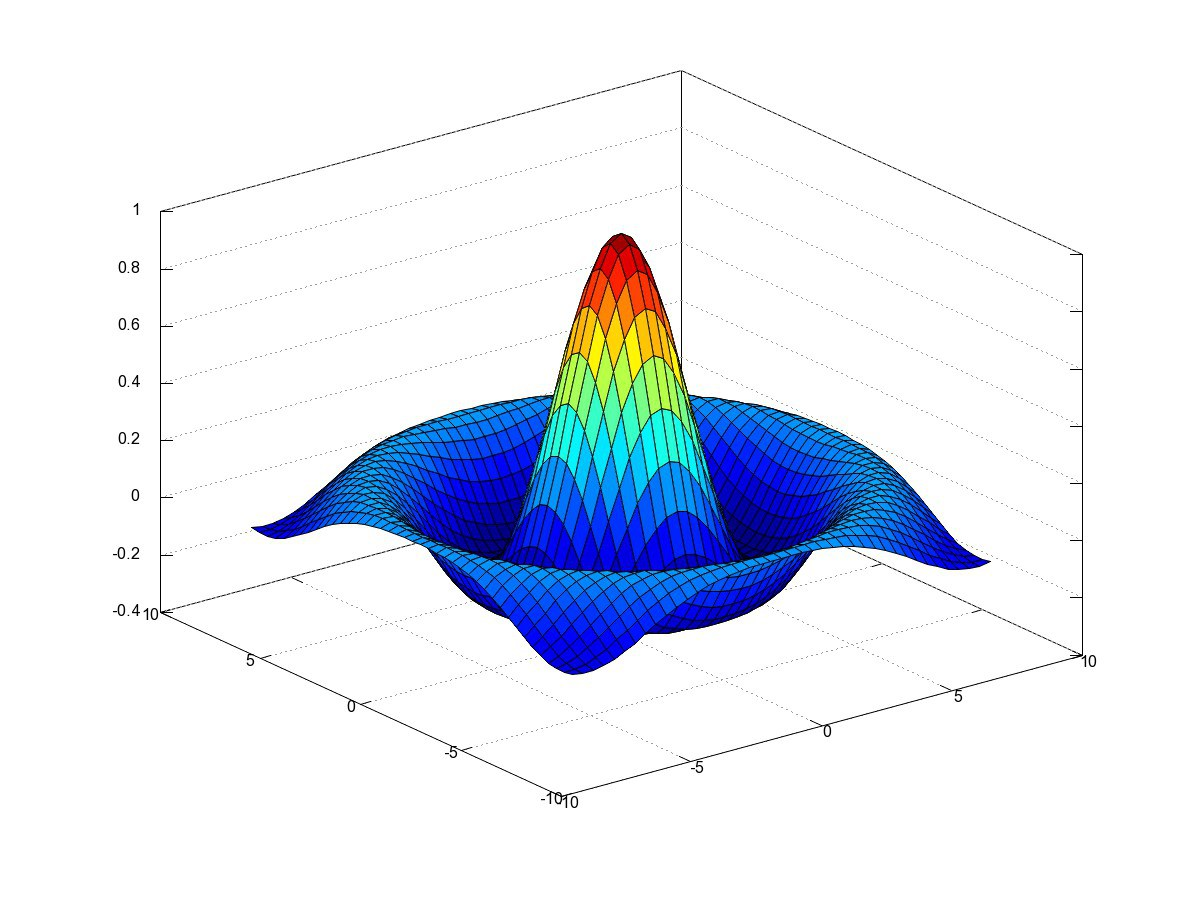
\includegraphics[width=2.6cm, height=1.7cm]{cover.jpg}
%\caption{Ogata - 5a Edicao - Fig. 1.1}
\label{Ogata_1_1}
\end{figure}
\end{frame}

\begin{frame}
\frametitle{Agenda da Apresentação} % Table of contents slide, comment this block out to remove it
\tableofcontents % Throughout your presentation, if you choose to use \section{} and \subsection{} commands, these will automatically be printed on this slide as an overview of your presentation
\end{frame}

%----------------------------------------------------------------------------------------
%	PRESENTATION SLIDES
%----------------------------------------------------------------------------------------

\section{Método Simplex}
\subsection{Descrição Geral}

\begin{frame}
	\frametitle{Histórico}
	\centering
	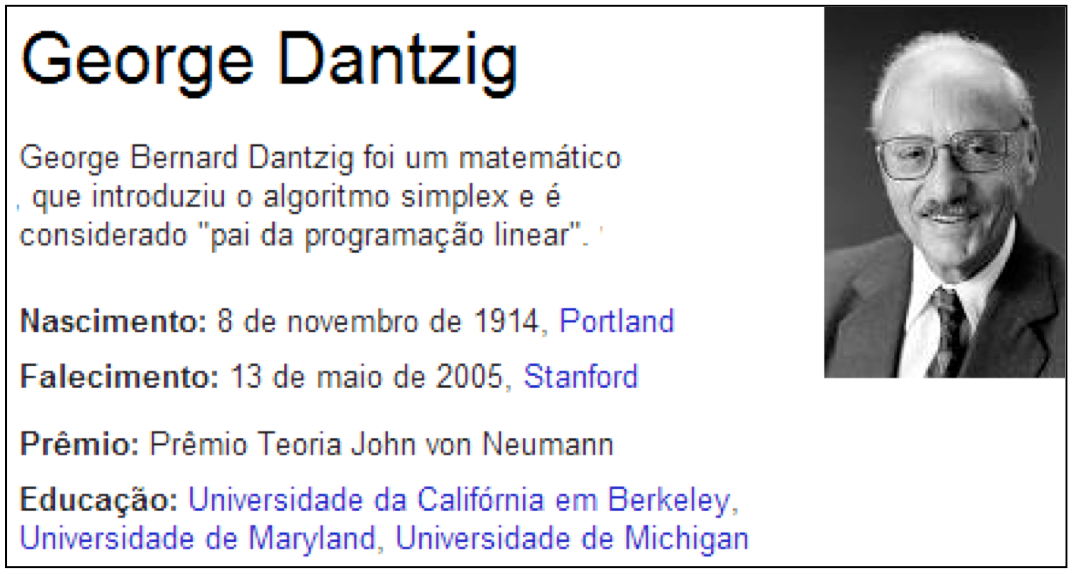
\includegraphics[width=8.5cm,height=5cm]{Dantzig.png}
\end{frame}

\begin{frame}
	\only<1>
	{
	\frametitle{Descrição Geral Simplex}
	}
	\only<2-6>
	{
	\frametitle{Descrição Geral Simplex \scriptsize (SBF = Solução Básica Factível)}
	}
	\centering
	\begin{tikzpicture} [
							auto, node distance = 2cm,
							decisao/.style = { diamond, draw, thick, fill=red!20,
							                   text width=3em, text badly centered,
							                   inner sep=1pt},
							bloco/.style   = { rectangle, draw, thick, fill=blue!20, 
												text width=10em, text centered,
							                   minimum height=1em },
							inicio/.style  = { ellipse, draw, fill=green!20,
							                   text width=5em, text centered },	
							line/.style   = { draw, -latex' },
						]

	    % Place nodes
	    \only<1-6>
	    {
	    \node [inicio] 				                        (init)      {\scriptsize Início: Forma Padrão};
	    }
	    \only<2-6>
	    {
	    \node [bloco,   below of=init]                      (solbasica) {\scriptsize Encontrar uma SBF Inicial};
	    }
	    \only<3-6>
	    {
	    \node [below of=solbasica] 							(null1)		{};
	    \node [decisao, below of=solbasica]                 (decide)    {\scriptsize Solução Ótima ?};
	    }
	    \only<4-6>
	    {
	    \node [bloco,   below of=decide]                    (melhora)   {\scriptsize Determinar uma SBF adjacente melhor};
	    }
	    \only<6>
	    {
	    \node [inicio,  right of=decide, node distance=4cm] (fim)       {\scriptsize Fim};
	    }
	    % Draw edges
	    \only<2-6>
	    {
	    \path [line] (init)      -- (solbasica);
	    }
	    \only<3-6>
	    {
	    \path [line] (solbasica) -- (decide);
	    }
	    \only<4-6>
	    {
	    \path [line] (decide)    -- node [near start] {\scriptsize não} (melhora);
	    }
	    \only<5-6>
	    {
	    \path [line] (melhora)    -| (-3,-2.5)  -- (0,-2.5) (null1);
		}
		\only<6>
		{
	    \path [line] (decide)    -- node [near start] {\scriptsize sim} (fim);
	    } 
	\end{tikzpicture}
\end{frame}

\subsection{Forma Padrão}
\begin{frame}
	\frametitle{Forma Padrão}
	\begin{table}
		\begin{tabular}{c c c}
			\only<1-6>
			{
				{\color{red} \textbf{Forma Geral/Original}} 
			} & &
			\only<2-6>
			{ 
				{\color{red} \textbf{Forma Padrão}} 
			} \\
			\only<1-6>
			{
				\cellcolor{blue!20}
				$
					\begin{matrix}
						\max Z = c^Tx \\
						\text{s.a.} \\
						Ax \{  =, \le, \ge \} b  \\
						x \ge 0  \\
					\end{matrix}
				$ 
			} &
			\only<2-6>
			{ 
				
\includegraphics[width=1.5cm,height=0.5cm]{seta.png}
			} &
			\only<2-6>
			{
				\cellcolor{blue!20}
				$
					\begin{matrix}
						\max Z = c^Tx \\
						\text{s.a.} \\
						Ax = b  \\
						x \ge 0  \\
					\end{matrix}
				$ 
			} \\
		\end{tabular}
	\end{table}
	
	\begin{table}
		\centering
		\begin{tabular}{c}
			\only<3-6>
			{
					
\includegraphics[width=0.3cm,height=0.3cm]{tick.png} \hspace{0.1cm}
					\scriptsize Os termos independentes das restrições devem ser não negativos $(b \ge 0)$. \\
			}
			\only<4-6>
			{

					
\includegraphics[width=0.3cm,height=0.3cm]{tick.png} \hspace{0.1cm}
					\scriptsize Todas as restrições na forma de \underline{igualdade} (exceção: não-negatividade). \\
			}
			\only<5-6>
			{
					
\includegraphics[width=0.3cm,height=0.3cm]{tick.png} \hspace{0.1cm}
					\scriptsize \underline{Não-negatividade}: As variáveis de decisão $x$ devem ser não negativas. \\
			}
			\only<6>
			{
					
\includegraphics[width=2.7cm,height=2.7cm]{importante.jpg} \\
					\cellcolor{green!50} \color{red} Sempre é possível escrever um PPL na forma padrão! \\
			}
			
		\end{tabular}
	\end{table}
\end{frame}

\begin{frame}
	\frametitle{Formulação Padrão} 
	\begin{mdframed}[backgroundcolor=blue!20] 
		\only<1>
		{
			\begin{equation*}
				\max z = c_1x_1 + c_2x_2 + \cdots + c_nx_n 
			\end{equation*}
			{\color{red}Sujeito a (restrições de igualdade)} 
			\begin{equation*}
				\begin{matrix}
					a_{11}x_1 + a_{12}x_2 + \cdots + c_{1n}x_n = b_1 \\
					a_{21}x_1 + a_{22}x_2 + \cdots + c_{2n}x_n = b_2 \\
					\vdots \\
					a_{m1}x_1 + a_{m2}x_2 + \cdots + c_{mn}x_n = b_n \\
					x_1, x_2, \cdots, x_n \ge 0 \\
				\end{matrix}
			\end{equation*}
			$n$ variáveis de decisão e $m$ restrições de igualdade.
		}
		\only<2>
		{
			\begin{equation*}
				\max z = \sum_{j=1}^{n}c_jx_j
			\end{equation*}
			{\color{red}Sujeito a (restrições de igualdade)} 
			\begin{equation*}
				\begin{matrix}
					\sum_{j=1}^{n}a_{ij} = b_i & \forall i = 1, 2, \cdots, m \\
					x_j \ge 0 & \forall j = 1, 2, \cdots, n \\
				\end{matrix}
			\end{equation*}
			$n$ variáveis de decisão e $m$ restrições de igualdade.
		}
		\only<3>
		{
			\begin{equation*} 
				\max z = \begin{bmatrix}
							c_1 & c_2 & \cdots & c_n \\
						 \end{bmatrix}
						 \begin{bmatrix}
							 x_1 \\
							 x_2 \\
							 \vdots \\
							 x_n \\
						 \end{bmatrix}
			\end{equation*}
			{\color{red}Sujeito a (restrições de igualdade)} 
			\begin{equation*}
				\begin{bmatrix}
						a_{11} & a_{12} & \cdots & a_{1n} \\
						a_{21} & a_{22} & \cdots & a_{2n} \\
						\vdots & \vdots & \ddots & \vdots \\
						a_{m1} & a_{m2} & \cdots & a_{mn} \\
				\end{bmatrix}
				\begin{bmatrix}
						x_1 \\
						x_2 \\
						\vdots \\
						x_n \\
				\end{bmatrix} = 
				\begin{bmatrix}
						b_1 \\
						b_2 \\
						\vdots \\
						b_m \\
				\end{bmatrix} \text{ e }
				\begin{bmatrix}
						x_1 \\
						x_2 \\
						\vdots \\
						x_n \\
				\end{bmatrix} \ge
				\begin{bmatrix}
						0 \\
						0 \\
						\vdots \\
						0 \\
				\end{bmatrix} 				
			\end{equation*}			
			$n$ variáveis de decisão e $m$ restrições de igualdade.
		}
		\only<4>
		{
			\begin{equation*} 
				\max z = \begin{bmatrix}
							c_1 & c_2 & \cdots & c_n \\
						 \end{bmatrix}_{\text{\color{red}1 x n}}
						 \begin{bmatrix}
							 x_1 \\
							 x_2 \\
							 \vdots \\
							 x_n \\
						 \end{bmatrix}_{\text{\color{red}n x 1}} 
			\end{equation*}
			{\color{red}Sujeito a (restrições de igualdade)} 
			\begin{equation*}
				\begin{bmatrix}
						a_{11} & a_{12} & \cdots & a_{1n} \\
						a_{21} & a_{22} & \cdots & a_{2n} \\
						\vdots & \vdots & \ddots & \vdots \\
						a_{m1} & a_{m2} & \cdots & a_{mn} \\
				\end{bmatrix}_{\text{\color{red}m x n}}
				\begin{bmatrix}
						x_1 \\
						x_2 \\
						\vdots \\
						x_n \\
				\end{bmatrix}_{\text{\color{red} n x 1}} = 
				\begin{bmatrix}
						b_1 \\
						b_2 \\
						\vdots \\
						b_m \\
				\end{bmatrix}_{\text{\color{red} m x 1}}  				
			\end{equation*}			
			$n$ variáveis de decisão e $m$ restrições de igualdade.
		}
		\only<5>
		{
			\begin{equation*} 
				\max z = \mathbf{c}^T \mathbf{x}
			\end{equation*}
			{\color{red}Sujeito a (restrições de igualdade)} 
			\begin{equation*}
				\begin{matrix}
					\mathbf{A_{eq}x} = \mathbf{B_{eq}}  \\
					\mathbf{x} \ge \mathbf{0}
				\end{matrix}
			\end{equation*}	
			$n$ variáveis de decisão e $m$ restrições de igualdade.		
		}		
	\end{mdframed}
	\only<5>
	{
	\vspace{0.3cm}
	\begin{equation*}
		\begin{matrix}
			\mathbf{c} = 	\begin{bmatrix}
									c_1 \\ c_2 \\ \vdots \\ c_n \\
							\end{bmatrix} &

			\mathbf{x} = 	\begin{bmatrix}
									x_1 \\ x_2 \\ \vdots \\ x_n \\
							\end{bmatrix} &

			\mathbf{B_{eq}} = 	\begin{bmatrix}
									b_1 \\ b_2 \\ \vdots \\ b_m \\
							\end{bmatrix} &

			\mathbf{A_{eq}} = 	\begin{bmatrix}
									a_{11} & a_{12} & \cdots & a_{1n} \\
									a_{21} & a_{22} & \cdots & a_{2n} \\
									\vdots & \vdots & \ddots & \vdots \\
									a_{m1} & a_{m2} & \cdots & a_{mn} \\
								\end{bmatrix} \\

		\end{matrix}
	\end{equation*}
	}
\end{frame}

\begin{frame}
	\frametitle{Relação entre Maximização e Minimização}
	\only<1>
	{
		\centering
		
\includegraphics[width=5cm,height=4cm]{up-down.jpg}
	}	
	\only<2>
	{
		\centering
		
\includegraphics[width=5cm,height=4cm]{up-down.jpg}
		\begin{itemize}
		\item Qualquer que seja o formato do PPL, sempre é possível transforma-lo no formato padrão apresentado.
		\item Como é a relação entre minimização e maximização?
		\end{itemize}
	}	
	\only<3>
	{
		\centering
		
\includegraphics[width=2.5cm,height=2cm]{up-down.jpg}
		\begin{mdframed}[backgroundcolor=blue!20] 
			\begin{equation*}
				\max z = \sum_{j=1}^{n}c_jx_j \Leftrightarrow \min (-z) = \sum_{j=1}^{n}(-c_j)x_j
			\end{equation*}
			\begin{equation*}
				\min z = \sum_{j=1}^{n}c_jx_j \Leftrightarrow \max (-z) = \sum_{j=1}^{n}(-c_j)x_j
			\end{equation*}
		\end{mdframed}
	}
\end{frame}

\begin{frame}
	\frametitle{Relação Entre Inequações e Equações}
	
	\only<1->
	{
	\underline{Restrições de Menor ou Igual} - Variável de Folga ($+S_i$)
	\begin{mdframed}[backgroundcolor=blue!20]
		\begin{equation*}
			\sum_{j-1}^{n}a_{ij}x_j \le b_i \Leftrightarrow
			\left\{ \begin{matrix}
						\sum_{j=1}^{n}a_{ij}x_j + S_i = b_i \\
						0 \le S_i \ge \infty
					\end{matrix}  
			\right.
		\end{equation*}
	\end{mdframed}	
	}
	
	\only<2>
	{
	\vspace{0.5cm}
	\underline{Restrições de Maior ou Igual} - Variável de Excesso ($-S_i$)
	\begin{mdframed}[backgroundcolor=red!20]
		\begin{equation*}
			\sum_{j-1}^{n}a_{ij}x_j \ge b_i \Leftrightarrow
			\left\{ \begin{matrix}
						\sum_{j=1}^{n}a_{ij}x_j - S_i = b_i \\
						0 \le S_i \ge \infty
					\end{matrix}  
			\right.
		\end{equation*}
	\end{mdframed}
	}
\end{frame}

\begin{frame}
	\frametitle{Tratamento de Limites das Variáveis}
	\only<1->
	{
	\underline{Limite Inferior ou \textit{Lower  Bound}}
	\begin{mdframed}[backgroundcolor=blue!20]
		\begin{equation*}
			x_j \ge LB \Leftrightarrow
			\left\{ \begin{matrix}
						x_j - LB = {x}'_j \Rightarrow x_j = {x}'_j + LB \\
						{x}'_j \ge 0
					\end{matrix}  
			\right.
		\end{equation*}
	\end{mdframed}	
	}
	
	\only<2->
	{
	\vspace{0.5cm}
	\underline{Limite Superior ou \textit{Upper  Bound}}
	\begin{mdframed}[backgroundcolor=red!20]
		\begin{equation*}
			x_j \le UB \Leftrightarrow
			\left\{ \begin{matrix}
						UB - x_j = {x}'_j \Rightarrow x_j = UB - {x}'_j  \\
						{x}'_j \ge 0
					\end{matrix}  
			\right.
		\end{equation*}
	\end{mdframed}
	}

	\only<3->
	{
	\vspace{0.5cm}
	\begin{mdframed}[backgroundcolor=green!20]
		\begin{equation*}
			- \infty \le x_j \le \infty \Leftrightarrow
			\left\{ \begin{matrix}
						x_j = {x}'_j - {x}''_j \\
						{x}'_j \ge 0 \text{ e } {x}''_j \ge 0  \\
					\end{matrix}  
			\right.
		\end{equation*}
	\end{mdframed}
	}
\end{frame}

\begin{frame}
	\frametitle{Exemplo 1}
	\begin{columns}
		\only<1-2>
		{
		\begin{column}{0.4\textwidth}
			\centering
			\begin{equation*}
				\overset{\text{\color{red}Forma Original}}
				{
					\overbrace{
								\begin{matrix}
									\max Z = 3x_1 + 2.5x_2 + 1.2x_3 \\
									\text{Sujeito a} \\
									\begin{matrix}
										x_1-2x_2+4x_3 & \le & 40 \\
										x_1+x_2+ 2x_3 & \le & 60 \\
										2x_1+3x_2+x_3 & \ge & 15 \\
									\end{matrix} \\
									x_1, x_2, x_3 \ge 0 \\
								\end{matrix}
							  }
				}
			\end{equation*}
		\end{column}
		}
		\only<2>
		{
		\begin{column}{0.6\textwidth}
			\centering
			\begin{equation*}
				\overset{\text{\color{red}Forma Padrão}}
				{
					\overbrace{
								\begin{matrix}
									\max Z = 3x_1 + 2.5x_2 + 1.2x_3 \\
									\text{Sujeito a} \\
									\begin{matrix}
										x_1-2x_2+4x_3 & \cellcolor{red!20}+x_4 &      &      & = & 40 \\
										x_1+x_2+2x_3  &      & \cellcolor{red!20}+x_5 &      & = & 60 \\
										2x_1+3x_2+x_3 &      &      & \cellcolor{red!20}-x_6 & = & 15 \\
									\end{matrix} \\
									x_1, x_2, x_3, x_4, x_5, x_6 \ge 0 \\
								\end{matrix}
							  }
				}
			\end{equation*}
		\end{column}
		}
	\end{columns}
\end{frame}

\begin{frame}
	\frametitle{Exemplo 2}
	\begin{columns}
		\begin{column}{0.5\textwidth}
		\begin{block}{Coloque o PPL abaixo na \underline{forma padrão}.}
			\begin{equation*}
				\begin{matrix}
					\scriptstyle \max Z = -2x_1+x_2+x_3-3x_4+x_5 \\
					\scriptstyle \text{Sujeito a:} \\
					\scriptstyle x_1+2x_2-x_3+x_4+3x_5 \ge 5 \\
					\scriptstyle 4x_1+x_3-2x_4-x_5 \le 0 \\
					\scriptstyle -2x_3+x_4+2x_5\ge -7 \\
					\scriptstyle 3x_1+x_2-x_4+x_5 = 8 \\
					\scriptstyle x_3 \le 0 \\
					\scriptstyle x_4 \text{ qualquer} \\
					\scriptstyle x_1, x_2, x_5 \ge 0 \\
				\end{matrix}
			\end{equation*}
		\end{block}
		\end{column}
		\begin{column}{0.5\textwidth}
			\begin{exampleblock}{Resposta: PPL Escrito na \underline{Forma Padrão}.}
				\begin{equation*}
					\begin{matrix}
						\only<2-9>{\scriptstyle \max Z = -2x_1+x_2+x_3-3x_4+x_5 \\}
						\only<3-9>{\scriptstyle \text{Sujeito a:} \\}
						\only<3-9>{\scriptstyle x_1+2x_2-x_3+x_4+3x_5 {\color{red}-S_1} = 5 \\}
						\only<4-9>{\scriptstyle 4x_1+x_3-2x_4-x_5 {\color{red}+S_2} = 0 \\}
						\only<5-9>{\scriptstyle {\color{red}2x_3-x_4-2x_5 +S_3 = 7} \\}
						\only<6-9>{\scriptstyle 3x_1+x_2-x_4+x_5 = 8 \\}
						\only<7-9>{\scriptstyle {\color{red}x_3=-x'_3 } \\}
						\only<8-9>{\scriptstyle {\color{red}x_4 = x'_4 - x''_4} \\}
						\only<9-9>{\scriptstyle x_1, x_2, {\color{red}x'_3, x'_4, x''_4, S_1, S_2, S_3,} x_5 \ge 0 \\}

						\only<10>{\scriptstyle \max Z = -2x_1+x_2{\color{red}-x'_3}-3{\color{red}(x'_4 - x''_4)}+x_5 \\}
						\only<10>{\scriptstyle \text{Sujeito a:} \\}
						\only<10>{\scriptstyle x_1+2x_2{+x'_3}{\color{red}+x'_4 - x''_4}+3x_5 {\color{red}-S_1} = 5 \\}
						\only<10>{\scriptstyle 4x_1{-x'_3}-2{\color{red}(x'_4 - x''_4)}-x_5 {\color{red}+S_2} = 0 \\}
						\only<10>{\scriptstyle {\color{red}-2{\color{red}x'_3}-{\color{red}(x'_4 - x''_4)}-2x_5 +S_3 = 7} \\}
						\only<10>{\scriptstyle 3x_1+x_2-{\color{red}(x'_4 - x''_4)}+x_5 = 8 \\}
						\only<10>{\scriptstyle x_1, x_2, {\color{red}x'_3, x'_4, x''_4, S_1, S_2, S_3,} x_5 \ge 0 \\}


					\end{matrix}
				\end{equation*}
			\end{exampleblock}
		\end{column}
	\end{columns}
\end{frame}

\begin{frame}[fragile]
	\frametitle{Exemplo 2}
	\begin{columns}
		\begin{column}{0.5\textwidth}
		\begin{block}{Coloque o PPL abaixo na \underline{forma padrão}.}
			\begin{equation*}
				\begin{matrix}
					\scriptstyle \max Z = -2x_1+x_2+x_3-3x_4+x_5 \\
					\scriptstyle \text{Sujeito a:} \\
					\scriptstyle x_1+2x_2-x_3+x_4+3x_5 \ge 5 \\
					\scriptstyle 4x_1+x_3-2x_4-x_5 \le 0 \\
					\scriptstyle -2x_3+x_4+2x_5\ge -7 \\
					\scriptstyle 3x_1+x_2-x_4+x_5 = 8 \\
					\scriptstyle x_3 \le 0 \\
					\scriptstyle x_4 \text{ qualquer} \\
					\scriptstyle x_1, x_2, x_5 \ge 0 \\
				\end{matrix}
			\end{equation*}
		\end{block}
		\end{column}
		\begin{column}{0.5\textwidth}
			\begin{block}{Programa em Matlab}
				\begin{lstlisting}[basicstyle=\tiny]  
clear all; close all; clc;
c = -[-2 1 1 -3 1];
A = [-1 -2 1 -1 -3; ...
      4  0 1 -2 -1; ...
      0  0 2 -1 -2];
B = [-5; 0 ; 7];
Aeq = [3 1 0 -1 1];
Beq = 8;
LB = [0     0 -inf -inf   0]; 
UB = [inf inf    0 inf  inf];
[x,fval, exitflag] = linprog(c,A,B,Aeq,Beq,LB,UB);
				\end{lstlisting}
			\end{block}
		\end{column}
	\end{columns}
\end{frame}

\begin{frame}
	\frametitle{Exemplo 2}
	\begin{columns}
		\begin{column}{0.5\textwidth}
		\begin{block}{Coloque o PPL abaixo na \underline{forma padrão}.}
			\begin{equation*}
				\begin{matrix}
					\scriptstyle \max Z = -2x_1+x_2+x_3-3x_4+x_5 \\
					\scriptstyle \text{Sujeito a:} \\
					\scriptstyle x_1+2x_2-x_3+x_4+3x_5 \ge 5 \\
					\scriptstyle 4x_1+x_3-2x_4-x_5 \le 0 \\
					\scriptstyle -2x_3+x_4+2x_5\ge -7 \\
					\scriptstyle 3x_1+x_2-x_4+x_5 = 8 \\
					\scriptstyle x_3 \le 0 \\
					\scriptstyle x_4 \text{ qualquer} \\
					\scriptstyle x_1, x_2, x_5 \ge 0 \\
				\end{matrix}
			\end{equation*}
		\end{block}
		\end{column}
		\begin{column}{0.5\textwidth}
			\begin{block}{Programa em Matlab}
				\only<1>
				{
					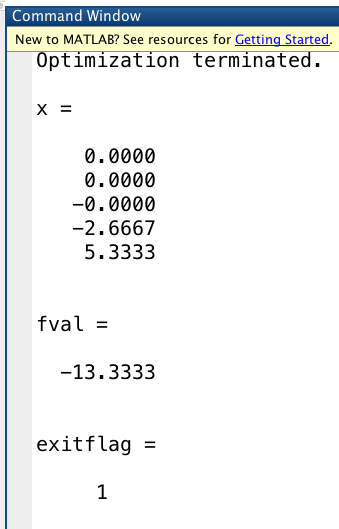
\includegraphics[width=4cm,height=6.5cm]{Exemplo2a.png}
				}
				\only<2>
				{
					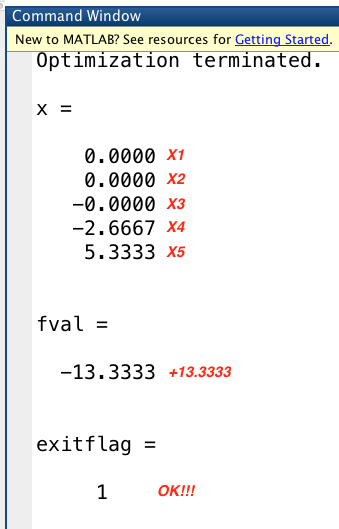
\includegraphics[width=4cm,height=6.5cm]{Exemplo2aLINHA.png}
				}
			\end{block}
		\end{column}
	\end{columns}
\end{frame}

\begin{frame}[fragile]
	\frametitle{Exemplo 2}
	\begin{columns}
		\begin{column}{0.5\textwidth}
			\begin{exampleblock}{Resposta: PPL Escrito na \underline{Forma Padrão}.}
				\begin{equation*}
					\begin{matrix}
						\scriptstyle \max Z = -2x_1+x_2{\color{red}-x'_3}-3{\color{red}(x'_4 - x''_4)}+x_5 \\
						\scriptstyle \text{Sujeito a:} \\
						\scriptstyle x_1+2x_2{+x'_3}{\color{red}+x'_4 - x''_4}+3x_5 {\color{red}-S_1} = 5 \\
						\scriptstyle 4x_1{-x'_3}-2{\color{red}(x'_4 - x''_4)}-x_5 {\color{red}+S_2} = 0 \\
						\scriptstyle {\color{red}-2{\color{red}x'_3}-{\color{red}(x'_4 - x''_4)}-2x_5 +S_3 = 7} \\
						\scriptstyle 3x_1+x_2-{\color{red}(x'_4 - x''_4)}+x_5 = 8 \\
						\scriptstyle x_1, x_2, {\color{red}x'_3, x'_4, x''_4, S_1, S_2, S_3,} x_5 \ge 0 \\
					\end{matrix}
				\end{equation*}
			\end{exampleblock}
		\end{column}
		\begin{column}{0.5\textwidth}
			\begin{block}{Programa em Matlab}
				\begin{lstlisting}[basicstyle=\tiny]  
clear all; close all; clc;
c = -[-2 1 -1 -3 +3 1 0 0 0];
A = [];
B = [];
Aeq = [ ...
  1 2  1  1 -1  3 -1 0 0; ...
  4 0 -1  2  2 -1  0 1 0; ...
  0 0 -2 -1  1 -2  0 0 1; ...
  3 1  0 -1  1  1  0 0 0; ...
  ];
Beq = [ 5; 0; 7; 8];
LB = [ 0 0 0 0 0 0 0 0]; 
UB = [inf inf inf inf inf inf inf];
[x,fval, exitflag] = linprog(c,A,B,Aeq,Beq,LB,UB);				
				\end{lstlisting}
			\end{block}
		\end{column}
	\end{columns}
\end{frame}

\begin{frame}
	\frametitle{Exemplo 2}
	\begin{columns}
		\begin{column}{0.5\textwidth}
			\begin{exampleblock}{Resposta: PPL Escrito na \underline{Forma Padrão}.}
				\begin{equation*}
					\begin{matrix}
						\scriptstyle \max Z = -2x_1+x_2{\color{red}-x'_3}-3{\color{red}(x'_4 - x''_4)}+x_5 \\
						\scriptstyle \text{Sujeito a:} \\
						\scriptstyle x_1+2x_2{+x'_3}{\color{red}+x'_4 - x''_4}+3x_5 {\color{red}-S_1} = 5 \\
						\scriptstyle 4x_1{-x'_3}-2{\color{red}(x'_4 - x''_4)}-x_5 {\color{red}+S_2} = 0 \\
						\scriptstyle {\color{red}-2{\color{red}x'_3}-{\color{red}(x'_4 - x''_4)}-2x_5 +S_3 = 7} \\
						\scriptstyle 3x_1+x_2-{\color{red}(x'_4 - x''_4)}+x_5 = 8 \\
						\scriptstyle x_1, x_2, {\color{red}x'_3, x'_4, x''_4, S_1, S_2, S_3,} x_5 \ge 0 \\
					\end{matrix}
				\end{equation*}
			\end{exampleblock}
		\end{column}
		\begin{column}{0.5\textwidth}
			\begin{block}{Programa em Matlab}
				\only<1>
				{
				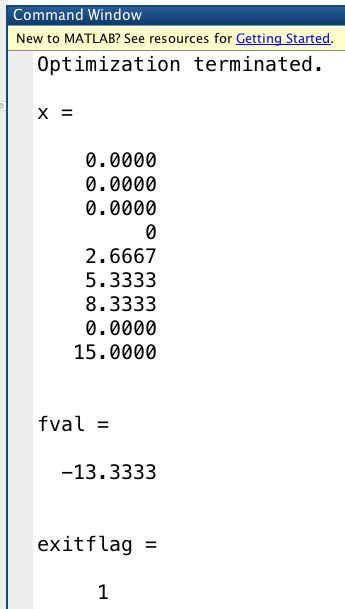
\includegraphics[width=4cm,height=6.5cm]{Exemplo2b.png}
				}
				\only<2>
				{
					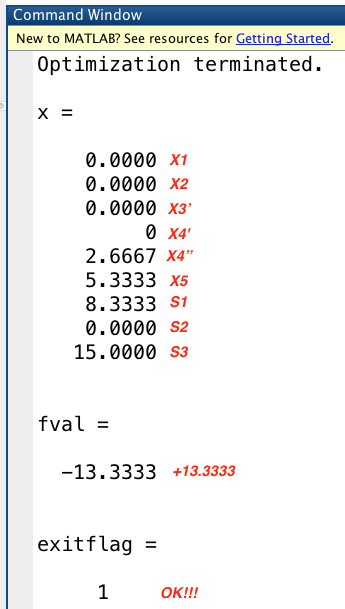
\includegraphics[width=4cm,height=6.5cm]{Exemplo2bLINHA.png}
				}
			\end{block}
		\end{column}
	\end{columns}
\end{frame}

\begin{frame}
	\frametitle{Solução Básica Inicial}
	\begin{block}{\underline{Observações}}
		\begin{enumerate}
			\item A passagem para forma padrão se faz pelo simples acréscimo de uma variável de folga ou excesso para cada inequação existente \pause
			\item {A forma padrão resultante consiste em um sistema que tenha uma \underline{\color{red}solução básica inicial} mais fácil de ser encontrada:} \pause
			\begin{itemize}
				\item[] {\color{red} Solução Básica Inicial (ESTRATÉGIA):} 
					\begin{table}
						\centering		
						\begin{tabular}{c}
							\scriptsize \cellcolor{yellow!70} Anular as variáveis originais \\
							\scriptsize \cellcolor{yellow!70} Obter os valores das variáveis de folga e excesso \\ \pause
						\end{tabular}
					\end{table}
			\end{itemize}
			\item As {\color{red}variáveis nulas} recebem o nome de {\color{red}NÃO BÁSICAS (VNB)} \\
			\item As {\color{red}variáveis não nulas} recebem o nome de {\color{red}BÁSICAS (VB)} \\
		\end{enumerate}
	\end{block}
\end{frame}

\begin{frame}
	\frametitle{Exemplo: Encontre uma {\color{red}\underline{SBF Inicial}} para:}
	\begin{columns}
		\begin{column}{0.3\textwidth}
			\begin{equation*}
				\begin{matrix}
					\scriptstyle \max Z = 3x_1 + 2,5x_2 + 1,2x_3 \\
					\scriptstyle \text{Sujeito a} \\
					\scriptstyle x_1 - 2x_2 + 4x_3 \le 40 \\
					\scriptstyle x_1 + x_2 + 2x_3 \le 60 \\
					\scriptstyle 2x_1 + 3x_2 + x_3 \ge 15 \\
					\scriptstyle x_1, x_2, x_3 \ge 0 \\
				\end{matrix}
			\end{equation*} \pause
		\end{column}
		\begin{column}{0.15\textwidth}
			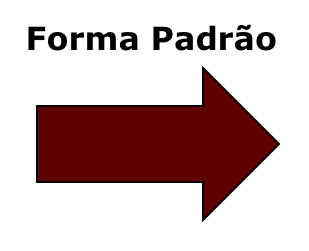
\includegraphics[width=2cm,height=1.5cm]{SetaFormaPadrao.png}
		\end{column}		
		\begin{column}{0.55\textwidth}
			\begin{mdframed}[backgroundcolor=yellow]
				\begin{equation*}
					\begin{matrix}
						\scriptstyle \max Z = 3x_1 + 2,5x_2 + 1,2x_3 \\
						\scriptstyle \text{Sujeito a} \\
					\end{matrix}
				\end{equation*}
				\only<2>
				{
					\begin{equation*}			
					\begin{matrix}
						\scriptstyle x_1 - 2x_2 + 4x_3 & \cellcolor{red!50} \scriptstyle+x_4 & & & \scriptstyle = 40 \\
						\scriptstyle x_1 + x_2 + 2x_3  & & \cellcolor{red!50} \scriptstyle+x_5 & & \scriptstyle = 60 \\
						\scriptstyle 2x_1 + 3x_2 + x_3 & & & \cellcolor{red!50} \scriptstyle-x_6 & \scriptstyle = 15 \\
					\end{matrix}
					\end{equation*}
					\begin{equation*}
					\scriptstyle x_1, x_2, x_3, x_4, x_5, x_6 \ge 0 
					\end{equation*}
				}			
				\only<3>
				{
					\begin{equation*}			
					\begin{matrix}
					\scriptstyle x_1 - 2x_2 + 4x_3 & \cellcolor{red!50} \scriptstyle+x_4 & & & \scriptstyle = 40 \\
					\scriptstyle x_1 + x_2 + 2x_3  & & \cellcolor{red!50} \scriptstyle+x_5 & & \scriptstyle = 60 \\
					\scriptstyle 2x_1 + 3x_2 + x_3 & & & \cellcolor{red!50} \scriptstyle-x_6 & \scriptstyle = 15 \\
					\scriptstyle \cellcolor{red!50} x_6 = -x_6^{*} & & & &\\
					\end{matrix}
					\end{equation*}
					\begin{equation*}
					\scriptstyle x_1, x_2, x_3, x_4, x_5, x_6 \ge 0 
					\end{equation*}
				}			
				\only<4-6>
				{
					\begin{equation*}			
					\begin{matrix}
					\scriptstyle x_1 - 2x_2 + 4x_3 & \cellcolor{red!50} \scriptstyle+x_4 & & & \scriptstyle = 40 \\
					\scriptstyle x_1 + x_2 + 2x_3  & & \cellcolor{red!50} \scriptstyle+x_5 & & \scriptstyle = 60 \\
					\scriptstyle 2x_1 + 3x_2 + x_3 & & & \cellcolor{red!50} \scriptstyle+x_6^{*} & \scriptstyle = 15 \\
					\end{matrix}
					\end{equation*}
					\begin{equation*}
					\scriptstyle x_1, x_2, x_3, x_4, x_5, x_6^{*} \ge 0 
					\end{equation*}
				}			
			\end{mdframed}
		\end{column}
	\end{columns}
	
	\only<5-6>
	{
		\begin{block}{Solução Básica Factível Inicial ???}
			\only<5>
			{
			\begin{itemize}
				\item As {\color{red}variáveis nulas} recebem o nome de {\color{red}NÃO BÁSICAS (VNB)}
				\item As {\color{red}variáveis não nulas} recebem o nome de {\color{red}BÁSICAS (VB)} 
			\end{itemize}
			}
			\only<6>
			{
				\begin{equation*}
					\begin{matrix}
						VNB = \{ x_1,x_2,x_3 \} \Leftrightarrow x_1=0, x_2=0, x_3=0 \\
						VB = \{ x_4,x_5,x_6^{*} \} \Leftrightarrow x_4=40, x_5=60, x_6^{*}=15 \\
						Z = 0 \\
					\end{matrix}
				\end{equation*}
			}
		\end{block}
	}

\end{frame}


\subsection{Passos da Resolução do PPL via Tableau Simplex}

\begin{frame}
	\frametitle{Passos da Resolução do PPL via Tableau Simplex}
	\begin{columns}
		\begin{column}{0.10\textwidth}
			\centering
			\only<2>
			{
				
\includegraphics[width=2.5cm,height=2.5cm]{number_1.jpg}\\
			}
			\only<3>
			{
				
\includegraphics[width=2.5cm,height=2.5cm]{number_2.jpg}\\
			}
			\only<4-5>
			{
				
\includegraphics[width=2.5cm,height=2.5cm]{number_3.jpg}\\
			}
			\only<6>
			{
				
\includegraphics[width=2.5cm,height=2.5cm]{number_4.jpg}\\
			}
		\end{column}
		\begin{column}{0.3\textwidth}
			\centering
			\begin{table}
				\only<1>
				{
				\begin{tabular}{c}
					\cellcolor{yellow}Problema em Análise \\
					$
						\begin{matrix}
							\max Z = 3x_1 + 5x_2 \\
							\text{Sujeito a:} \\
							x_1 \le 4 \\
							2x_2 \le 12 \\
							3x_1 + 2x_2 \le 18 \\
							x_1, x_2 \ge 0 \\
						\end{matrix} 	
					$ \\
				\end{tabular}
				}
				\only<2>
				{
				\begin{tabular}{c}
					\cellcolor{yellow}Problema em Análise \\
					\cellcolor{red!60}\scriptsize Reescrever a expressão da FOB \\ 
					$
						\begin{matrix}
							\color{red} \max Z - 3x_1 - 5x_2 = 0 \\
							\text{Sujeito a:} \\
							x_1 \le 4 \\
							2x_2 \le 12 \\
							3x_1 + 2x_2 \le 18 \\
							x_1, x_2 \ge 0 \\
						\end{matrix} 	
					$ \\
				\end{tabular}
				}		
				\only<3>
				{
				\begin{tabular}{c}
					\cellcolor{yellow}Problema em Análise \\
					\cellcolor{red!60}\scriptsize Problema na Forma Padrão \\ 
					$
						\begin{matrix}
							\color{red} \max Z - 3x_1 - 5x_2 = 0 \\
							\text{Sujeito a:} \\
							x_1 + {\color{red}S_1 =} 4 \\
							2x_2 + {\color{red}S_2 =} 12 \\
							3x_1 + 2x_2 + {\color{red}S_3 =} 18 \\
							x_1, x_2,{\color{red} S_1, S_2, S_3} \ge 0 \\
						\end{matrix} 	
					$ \\
				\end{tabular}
				}		
				\only<4-5>
				{
				\begin{tabular}{c}
					\cellcolor{yellow}Problema em Análise \\
					\cellcolor{red!60}\scriptsize Achar SBF Inicial \\
					$
						\begin{matrix}
							\color{red} \max Z - 3x_1 - 5x_2 = 0 \\
							\text{Sujeito a:} \\
							x_1 + {\color{red}S_1 =} 4 \\
							2x_2 + {\color{red}S_2 =} 12 \\
							3x_1 + 2x_2 + {\color{red}S_3 =} 18 \\
							x_1, x_2,{\color{red} S_1, S_2, S_3} \ge 0 \\
						\end{matrix} 	
					$ \\
					\hline
					$
					\begin{matrix}
						\cellcolor{red!60}S_1 = 4  & \cellcolor{red!60}x_1 = 0 \\
						\cellcolor{red!60}S_2 = 12 & \cellcolor{red!60}x_2 = 0 \\
						\cellcolor{red!60}S_3 = 18 & \cellcolor{red!60}Z = 0 \\
					\end{matrix}
					$ \\
					\hline
				\end{tabular}
				}						
				\only<6>
				{
				\begin{tabular}{c}
					\cellcolor{yellow}Problema em Análise \\
					\cellcolor{red!60}\scriptsize Montar o TABLEAU Simplex \\
					$
						\begin{matrix}
							\color{red} \max Z - 3x_1 - 5x_2 = 0 \\
							\text{Sujeito a:} \\
							x_1 + {\color{red}S_1 =} 4 \\
							2x_2 + {\color{red}S_2 =} 12 \\
							3x_1 + 2x_2 + {\color{red}S_3 =} 18 \\
							x_1, x_2,{\color{red} S_1, S_2, S_3} \ge 0 \\
						\end{matrix} 	
					$ \\
					\hline
					$
					\begin{matrix}
						\cellcolor{red!60}S_1 = 4  & \cellcolor{red!60}x_1 = 0 \\
						\cellcolor{red!60}S_2 = 12 & \cellcolor{red!60}x_2 = 0 \\
						\cellcolor{red!60}S_3 = 18 & \cellcolor{red!60}Z = 0 \\
					\end{matrix}
					$ \\
					\hline
				\end{tabular}
				}						
			\end{table}
		\end{column}
		\centering
		\begin{column}{0.4\textwidth}
			\centering
			\only<5>
			{
				\begin{tabular}{c}
					\hline
					$
						VNB = \{ x_1, x_2 \} 
					$ \\
					$
						VB = \{ S_1, S_2, S_3 \} 
					$ \\
					\hline
				\end{tabular}
				\begin{alertblock}{Atenção}
					A FOB deve ser sempre formada por VNB.
				\end{alertblock}
				
			}		
			\only<6>
			{
				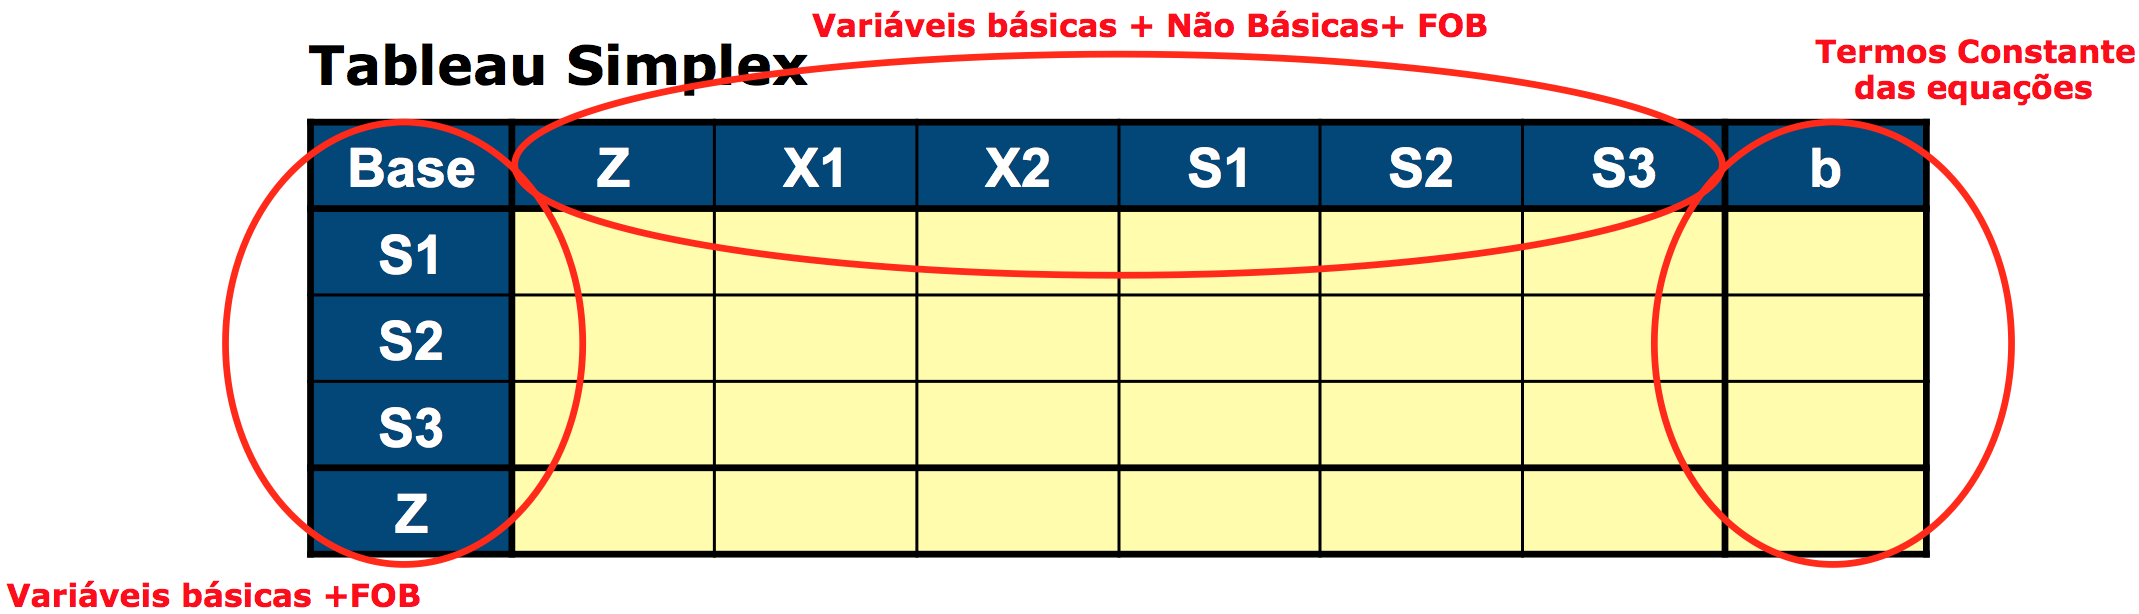
\includegraphics[width=5.2cm,height=2cm]{tableau.png}	
			}		
		\end{column}
	\end{columns}
\end{frame}

\begin{frame}
	\frametitle{
\includegraphics[width=0.6cm,height=0.6cm]{number_4.jpg} \hspace{0.2cm} Passos da Resolução do PPL via Tableau Simplex}
		
	\begin{table}
		\begin{tabular}{c}
			\cellcolor{yellow}Problema em Análise \\
			$
				\begin{matrix}
					\color{red} \max Z - 3x_1 - 5x_2 = 0 \\
					\text{Sujeito a:} \\
					x_1 + {\color{red}S_1 =} 4 \\
					2x_2 + {\color{red}S_2 =} 12 \\
					3x_1 + 2x_2 + {\color{red}S_3 =} 18 \\
					x_1, x_2,{\color{red} S_1, S_2, S_3} \ge 0 \\
				\end{matrix} 	
			$ 
		\end{tabular}
	\end{table}
		
	\begin{table}		
		\caption{\textbf{Tableau Simplex} \color{red} \scriptsize Preenchimento pelas linhas do Tableau	}
		\begin{tabular}{c | c | c | c | c | c | c | c | c | }
			\cline{2-9} 
			&\cellcolor{blue!100} \color{white}Base 
			&\cellcolor{blue!100} \color{white}Z 
			&\cellcolor{blue!100} \color{white} $X_1$ 
			&\cellcolor{blue!100} \color{white} $ X_2$ 
			&\cellcolor{blue!100} \color{white} $S_1$ 
			&\cellcolor{blue!100} \color{white} $S_2$ 
			&\cellcolor{blue!100} \color{white} $S_3$ 
			&\cellcolor{blue!100} \color{white} b \\
			\cline{2-9}
			\color{red} \scriptsize Restr.(1)  
			& \cellcolor{blue!100} \color{white} $S_1$
			& \cellcolor{yellow!50} \only<2->{$0$}
			& \cellcolor{yellow!50} \only<3->{$1$}
			& \cellcolor{yellow!50} \only<4->{$0$}
			& \cellcolor{yellow!50} \only<5->{$1$}
			& \cellcolor{yellow!50} \only<6->{$0$}
			& \cellcolor{yellow!50} \only<7->{$0$}
			& \cellcolor{yellow!50} \only<8->{$4$} \\
			\cline{2-9} 
			\color{red} \scriptsize Restr.(2)  
			& \cellcolor{blue!100} \color{white} $S_2$
			& \cellcolor{yellow!50} \only<9->{$0$}
			& \cellcolor{yellow!50} \only<10->{$0$}
			& \cellcolor{yellow!50} \only<11->{$2$}
			& \cellcolor{yellow!50} \only<12->{$0$}			
			& \cellcolor{yellow!50} \only<13->{$1$}
			& \cellcolor{yellow!50} \only<14->{$0$}
			& \cellcolor{yellow!50} \only<15->{$12$} \\
			\cline{2-9} 
			\color{red} \scriptsize Restr.(3)  
			& \cellcolor{blue!100} \color{white} $S_3$
			& \cellcolor{yellow!50} \only<16->{$0$}
			& \cellcolor{yellow!50} \only<17->{$3$}
			& \cellcolor{yellow!50} \only<18->{$2$}
			& \cellcolor{yellow!50} \only<19->{$0$}
			& \cellcolor{yellow!50} \only<20->{$0$}
			& \cellcolor{yellow!50} \only<21->{$1$}
			& \cellcolor{yellow!50} \only<22->{$18$} \\
			\cline{2-9}
			\color{red} \scriptsize FOB
			\footnote{\color{red}\textbf{A FOB deve ser sempre formada por VNB}}
			& \cellcolor{blue!100} \color{white} $Z$
			& \cellcolor{yellow!50} \only<22->{$1$}
			& \cellcolor{yellow!50} \only<22->{$-3$}
			& \cellcolor{yellow!50} \only<22->{$-5$}
			& \cellcolor{yellow!50} \only<22->{$0$}
			& \cellcolor{yellow!50} \only<22->{$0$}
			& \cellcolor{yellow!50} \only<22->{$0$}
			& \cellcolor{yellow!50} \only<22->{$0$} \\
			\cline{2-9} 
		\end{tabular}
	\end{table}
\end{frame}

\section{Fluxograma do Tableau}
\subsection{Problema de Maximização}

\begin{frame}
\frametitle{Fluxograma Tableau Simplex - \color{pink!100} MAXIMIZAÇÃO}
	\centering
	\begin{tikzpicture} [
							auto, node distance = 2cm,
							decisao/.style = { diamond, draw, shape aspect=2, thick, fill=red!20,
							                   text width=6em, text badly centered,
							                   inner sep=1pt},
							bloco/.style   = { rectangle, draw, thick, fill=blue!20, 
												text width=5em, text centered,
							                   minimum height=1em },
							bloco2/.style   = { rectangle, draw, thick, fill=blue!20, 
												text width=5em, text centered,
							                   minimum height=1em, node distance = 4.2cm },
							extremo/.style  = { ellipse, draw, fill=green!20,
							                   text width=5em, text centered,
							                   minimum height=2em },	
							line/.style   = { draw, -latex' },
							goto/.style = {circle, draw, fill=yellow!60, text width=1em,
										   text centered, node distance = 1.8cm},
						    bullet/.style = {rectangle, draw, thick, fill=red!80, 
						    				text width=9em, text centered,
						    				minimum height=1em},
						]

	
		\node [extremo] (inic) {\tiny INÍCIO}; \pause
		
		\node [bloco, below of = inic] (sbfi) {\tiny Montar Tableau Simplex com SBF Inicial};
		\path [line] (inic) -- (sbfi); \pause
		
		\node [decisao, below of = sbfi] (conv) {\tiny Existe Custo (coeficientes) $<$ 0 ?} ;
		\path [line] (sbfi) -- (conv); \pause
		
		\node[bloco, below of = conv] (otimo) {\tiny Solução Ótima};
		\path [line] (conv) -- node [near start] {\scriptsize \color{red} não} (otimo); 
	    \node [extremo] at (2,-7.2) (fim) {\tiny Fim};	
	    \path [line] (otimo) |- (2,-6.5) -- (fim); \pause

		\node[bloco2, right of = inic] (escolhe) {\tiny Escolher Variável Entrar na Base};
		\path [line] (conv) -| (2.2, 0) node [near start] {\scriptsize \color{red} sim} -- (escolhe); \pause
		
		\node[bloco, below of = escolhe] (razao) {\tiny Calcular Razão $ \frac{b_i}{coluna}$};
		\path [line] (escolhe) -- (razao); \pause

		\node [decisao, below of = razao] (finito) {\tiny Existe Razão $\ge 0$ finita ?} ;
		\path [line] (razao) -- (finito); \pause
		
		\node[bloco, below of = finito] (ilimit) {\tiny Solução Ilimitada};
		\path [line] (finito) -- node [near start] {\scriptsize \color{red} não} (ilimit); 
		\path [line] (ilimit) |- (2,-6.5) -- (fim); \pause

		\node[bloco2, right of = razao] (saibase) {\tiny Escolher Variável Sair da Base};
		\path [line] (finito) -| (6.2, -2) node [near start] {\scriptsize \color{red} sim} -- (saibase); \pause
		
		\node[bloco, below of = saibase] (swap) {\tiny Troca Base e Recalc. Tableau};
		\path[line] (saibase) -- (swap); \pause
		
		\node[goto, below of = swap] (pula_a) {\tiny 1};
		\node[goto, left of = sbfi] (pula_b) {\tiny 1};
		\path[line] (pula_b) -- (conv);
		\path[line] (swap) -- (pula_a); \pause
		
		%\only<2>
		%{
			\node[bullet] at (7.5,-0.2) (obs1) {\tiny Coef mais negativo FOB};
			\path[line] (obs1) -- (escolhe);
		%}

		%\only<3>
		%{
			\node[bullet] at (7.7,-1) (obs2) {\tiny Menor Razão Positiva};
			\path[line] (obs2) -- (saibase);
		%}
		
	\end{tikzpicture}	
\end{frame}

\begin{frame}
	\frametitle{
\includegraphics[width=0.6cm,height=0.6cm]{number_4.jpg} \hspace{0.2cm} Passos da Resolução do PPL via Tableau Simplex}

	\only<1-2>
	{		
		\begin{table}		
			\begin{tabular}{c c c c c c c c c c c}
				\cline{1-8} 
				\cellcolor{blue!100} \color{white} \scriptsize Base 
				&\cellcolor{blue!100} \color{white} \scriptsize Z 
				&\cellcolor{blue!100} \color{white} $\scriptstyle X_1$ 
				&\cellcolor{blue!100} \color{white} $\scriptstyle X_2$ 
				&\cellcolor{blue!100} \color{red} $\scriptstyle S_1$ 
				&\cellcolor{blue!100} \color{red} $\scriptstyle S_2$ 
				&\cellcolor{blue!100} \color{red} $\scriptstyle S_3$ 
				&\cellcolor{blue!100} \color{white} \scriptsize b
				&
				&
				& \\
				\cline{1-8}
				\cellcolor{blue!100} \color{red} $\scriptstyle S_1$
				& \cellcolor{yellow!50} $\scriptstyle 0$
				& \cellcolor{yellow!50} $\scriptstyle 1$
				& \cellcolor{yellow!50} $\scriptstyle 0$
				& \cellcolor{yellow!50} $\scriptstyle 1$
				& \cellcolor{yellow!50} $\scriptstyle 0$
				& \cellcolor{yellow!50} $\scriptstyle 0$
				& \cellcolor{yellow!50} $\scriptstyle 4$
				&
				&
				& \\
				\cline{1-8} 
			    \cellcolor{blue!100} \color{red} $\scriptstyle S_2$
				& \cellcolor{yellow!50} $\scriptstyle 0$
				& \cellcolor{yellow!50} $\scriptstyle 0$
				& \cellcolor{yellow!50} $\scriptstyle 2$
				& \cellcolor{yellow!50} $\scriptstyle 0$			
				& \cellcolor{yellow!50} $\scriptstyle 1$
				& \cellcolor{yellow!50} $\scriptstyle 0$
				& \cellcolor{yellow!50} $\scriptstyle 12$
				&
				&
				& \\
				\cline{1-8} 
				\cellcolor{blue!100} \color{red} $\scriptstyle S_3$
				& \cellcolor{yellow!50} $\scriptstyle 0$
				& \cellcolor{yellow!50} $\scriptstyle 3$
				& \cellcolor{yellow!50} $\scriptstyle 2$
				& \cellcolor{yellow!50} $\scriptstyle 0$
				& \cellcolor{yellow!50} $\scriptstyle 0$
				& \cellcolor{yellow!50} $\scriptstyle 1$
				& \cellcolor{yellow!50} $\scriptstyle 18$
				&
				&
				& \\
				\cline{1-8}
				\cellcolor{blue!100} \color{white} $\scriptstyle Z$
				& \cellcolor{yellow!50} $\scriptstyle 1$
				& \cellcolor{yellow!50} $\scriptstyle -3$
				& \cellcolor{yellow!50} $\scriptstyle -5$
				& \cellcolor{yellow!50} $\scriptstyle 0$
				& \cellcolor{yellow!50} $\scriptstyle 0$
				& \cellcolor{yellow!50} $\scriptstyle 0$
				& \cellcolor{yellow!50} $\scriptstyle 0$ 
				&
				&
				& \\
				\cline{1-8}
			\end{tabular}
		\end{table}			
	}	
	\only<3>
	{		
		\begin{table}		
			\begin{tabular}{c c c c c c c c c c c}
				\cline{1-8} 
				\cellcolor{blue!100} \color{white} \scriptsize Base 
				&\cellcolor{blue!100} \color{white} \scriptsize Z 
				&\cellcolor{blue!100} \color{white} $\scriptstyle X_1$ 
				&\cellcolor{blue!100} \color{white} $\scriptstyle X_2$ 
				&\cellcolor{blue!100} \color{red} $\scriptstyle S_1$ 
				&\cellcolor{blue!100} \color{red} $\scriptstyle S_2$ 
				&\cellcolor{blue!100} \color{red} $\scriptstyle S_3$ 
				&\cellcolor{blue!100} \color{white} \scriptsize b
				&
				&
				& \\
				\cline{1-8}
				\cellcolor{blue!100} \color{red} $\scriptstyle S_1$
				& \cellcolor{yellow!50} $\scriptstyle 0$
				& \cellcolor{yellow!50} $\scriptstyle 1$
				& \cellcolor{gray!50} $\scriptstyle 0$
				& \cellcolor{yellow!50} $\scriptstyle 1$
				& \cellcolor{yellow!50} $\scriptstyle 0$
				& \cellcolor{yellow!50} $\scriptstyle 0$
				& \cellcolor{yellow!50} $\scriptstyle 4$
				&
				&
				& \\
				\cline{1-8} 
				\cellcolor{blue!100} \color{red} $\scriptstyle S_2$
				& \cellcolor{yellow!50} $\scriptstyle 0$
				& \cellcolor{yellow!50} $\scriptstyle 0$
				& \cellcolor{gray!50} $\scriptstyle 2$
				& \cellcolor{yellow!50} $\scriptstyle 0$			
				& \cellcolor{yellow!50} $\scriptstyle 1$
				& \cellcolor{yellow!50} $\scriptstyle 0$
				& \cellcolor{yellow!50} $\scriptstyle 12$
				&
				&
				& \\
				\cline{1-8} 
				\cellcolor{blue!100} \color{red} $\scriptstyle S_3$
				& \cellcolor{yellow!50} $\scriptstyle 0$
				& \cellcolor{yellow!50} $\scriptstyle 3$
				& \cellcolor{gray!50} $\scriptstyle 2$
				& \cellcolor{yellow!50} $\scriptstyle 0$
				& \cellcolor{yellow!50} $\scriptstyle 0$
				& \cellcolor{yellow!50} $\scriptstyle 1$
				& \cellcolor{yellow!50} $\scriptstyle 18$
				&
				&
				& \\
				\cline{1-8}
				\cellcolor{blue!100} \color{white} $\scriptstyle Z$
				& \cellcolor{yellow!50} $\scriptstyle 1$
				& \cellcolor{yellow!50} $\scriptstyle -3$
				& \cellcolor{gray!50} $\scriptstyle -5$
				& \cellcolor{yellow!50} $\scriptstyle 0$
				& \cellcolor{yellow!50} $\scriptstyle 0$
				& \cellcolor{yellow!50} $\scriptstyle 0$
				& \cellcolor{yellow!50} $\scriptstyle 0$ 
				&
				&
				& \\
				\cline{1-8} 
				& 
				& 
				& 
\includegraphics[width=0.3cm,height=0.3cm]{setacima.jpg}
				& 
				& 
				& 
				&  
				&
				&
				& \\ 
				& 
				& 
				& \scriptsize \color{red} Entra 
				& 
				& 
				& 
				&  
				&
				&
				& \\
				& 
				& 
				& \scriptsize \color{red} Base 
				& 
				& 
				& 
				&  
				&
				&
				& \\

			\end{tabular}
		\end{table}			
	}	
	\only<4>
	{		
		\begin{table}		
			\begin{tabular}{c c c c c c c c c c c}
				\cline{1-8} 
				\cellcolor{blue!100} \color{white} \scriptsize Base 
				&\cellcolor{blue!100} \color{white} \scriptsize Z 
				&\cellcolor{blue!100} \color{white} $\scriptstyle X_1$ 
				&\cellcolor{blue!100} \color{white} $\scriptstyle X_2$ 
				&\cellcolor{blue!100} \color{red} $\scriptstyle S_1$ 
				&\cellcolor{blue!100} \color{red} $\scriptstyle S_2$ 
				&\cellcolor{blue!100} \color{red} $\scriptstyle S_3$ 
				&\cellcolor{blue!100} \color{white} \scriptsize b
				&
				&
				& \\
				\cline{1-8}
				\cellcolor{blue!100} \color{red} $\scriptstyle S_1$
				& \cellcolor{yellow!50} $\scriptstyle 0$
				& \cellcolor{yellow!50} $\scriptstyle 1$
				& \cellcolor{gray!50} $\scriptstyle 0$
				& \cellcolor{yellow!50} $\scriptstyle 1$
				& \cellcolor{yellow!50} $\scriptstyle 0$
				& \cellcolor{yellow!50} $\scriptstyle 0$
				& \cellcolor{gray!50} $\scriptstyle 4$
				& $ \scriptstyle \color{red} 4 \div 0 = \infty $
				&
				& \\
				\cline{1-8} 
				\cellcolor{blue!100} \color{red} $\scriptstyle S_2$
				& \cellcolor{yellow!50} $\scriptstyle 0$
				& \cellcolor{yellow!50} $\scriptstyle 0$
				& \cellcolor{gray!50} $\scriptstyle 2$
				& \cellcolor{yellow!50} $\scriptstyle 0$			
				& \cellcolor{yellow!50} $\scriptstyle 1$
				& \cellcolor{yellow!50} $\scriptstyle 0$
				& \cellcolor{gray!50} $\scriptstyle 12$
				& $ \scriptstyle \color{red} 12 \div 2 = +6 $
				&
				& \\
				\cline{1-8} 
				\cellcolor{blue!100} \color{red} $\scriptstyle S_3$
				& \cellcolor{yellow!50} $\scriptstyle 0$
				& \cellcolor{yellow!50} $\scriptstyle 3$
				& \cellcolor{gray!50} $\scriptstyle 2$
				& \cellcolor{yellow!50} $\scriptstyle 0$
				& \cellcolor{yellow!50} $\scriptstyle 0$
				& \cellcolor{yellow!50} $\scriptstyle 1$
				& \cellcolor{gray!50} $\scriptstyle 18$
				& $ \scriptstyle \color{red} 18 \div 2 = +9 $
				&
				& \\
				\cline{1-8}
				\cellcolor{blue!100} \color{white} $\scriptstyle Z$
				& \cellcolor{yellow!50} $\scriptstyle 1$
				& \cellcolor{yellow!50} $\scriptstyle -3$
				& \cellcolor{gray!50} $\scriptstyle -5$
				& \cellcolor{yellow!50} $\scriptstyle 0$
				& \cellcolor{yellow!50} $\scriptstyle 0$
				& \cellcolor{yellow!50} $\scriptstyle 0$
				& \cellcolor{gray!50} $\scriptstyle 0$ 
				&
				&
				& \\
				\cline{1-8} 
				& 
				& 
				& 
\includegraphics[width=0.3cm,height=0.3cm]{setacima.jpg}
				& 
				& 
				& 
				&  
				&
				&
				& \\ 
				& 
				& 
				& \scriptsize \color{red} Entra 
				& 
				& 
				& 
				&  
				&
				&
				& \\
				& 
				& 
				& \scriptsize \color{red} Base 
				& 
				& 
				& 
				&  
				&
				&
				& \\

			\end{tabular}
		\end{table}			
	}	
	\only<5>
	{		
		\begin{table}		
			\begin{tabular}{c c c c c c c c c c c}
				\cline{1-8} 
				\cellcolor{blue!100} \color{white} \scriptsize Base 
				&\cellcolor{blue!100} \color{white} \scriptsize Z 
				&\cellcolor{blue!100} \color{white} $\scriptstyle X_1$ 
				&\cellcolor{blue!100} \color{white} $\scriptstyle X_2$ 
				&\cellcolor{blue!100} \color{red} $\scriptstyle S_1$ 
				&\cellcolor{blue!100} \color{red} $\scriptstyle S_2$ 
				&\cellcolor{blue!100} \color{red} $\scriptstyle S_3$ 
				&\cellcolor{blue!100} \color{white} \scriptsize b
				&
				&
				& \\
				\cline{1-8}
				\cellcolor{blue!100} \color{red} $\scriptstyle S_1$
				& \cellcolor{yellow!50} $\scriptstyle 0$
				& \cellcolor{yellow!50} $\scriptstyle 1$
				& \cellcolor{gray!50} $\scriptstyle 0$
				& \cellcolor{yellow!50} $\scriptstyle 1$
				& \cellcolor{yellow!50} $\scriptstyle 0$
				& \cellcolor{yellow!50} $\scriptstyle 0$
				& \cellcolor{gray!50} $\scriptstyle 4$
				& $ \scriptstyle \color{red} 4 \div 0 = \infty $
				&
				& \\
				\cline{1-8} 
				\cellcolor{blue!100} \color{red} $\scriptstyle S_2$
				& \cellcolor{yellow!50} $\scriptstyle 0$
				& \cellcolor{yellow!50} $\scriptstyle 0$
				& \cellcolor{gray!50} $\scriptstyle 2$
				& \cellcolor{yellow!50} $\scriptstyle 0$			
				& \cellcolor{yellow!50} $\scriptstyle 1$
				& \cellcolor{yellow!50} $\scriptstyle 0$
				& \cellcolor{gray!50} $\scriptstyle 12$
				& $ \scriptstyle \color{red} 12 \div 2 = +6 $
				& 
\includegraphics[width=0.3cm,height=0.2cm]{setaesquerda.jpg}
				& \\
				\cline{1-8} 
				\cellcolor{blue!100} \color{red} $\scriptstyle S_3$
				& \cellcolor{yellow!50} $\scriptstyle 0$
				& \cellcolor{yellow!50} $\scriptstyle 3$
				& \cellcolor{gray!50} $\scriptstyle 2$
				& \cellcolor{yellow!50} $\scriptstyle 0$
				& \cellcolor{yellow!50} $\scriptstyle 0$
				& \cellcolor{yellow!50} $\scriptstyle 1$
				& \cellcolor{gray!50} $\scriptstyle 18$
				& $ \scriptstyle \color{red} 18 \div 2 = +9 $
				& 
\includegraphics[width=0.3cm,height=0.2cm]{setaesquerda.jpg}
				& \\
				\cline{1-8}
				\cellcolor{blue!100} \color{white} $\scriptstyle Z$
				& \cellcolor{yellow!50} $\scriptstyle 1$
				& \cellcolor{yellow!50} $\scriptstyle -3$
				& \cellcolor{gray!50} $\scriptstyle -5$
				& \cellcolor{yellow!50} $\scriptstyle 0$
				& \cellcolor{yellow!50} $\scriptstyle 0$
				& \cellcolor{yellow!50} $\scriptstyle 0$
				& \cellcolor{gray!50} $\scriptstyle 0$ 
				&
				&
				& \\
				\cline{1-8} 
				& 
				& 
				& 
\includegraphics[width=0.3cm,height=0.3cm]{setacima.jpg}
				& 
				& 
				& 
				&  
				&
				&
				& \\ 
				& 
				& 
				& \scriptsize \color{red} Entra 
				& 
				& 
				& 
				&  
				&
				&
				& \\
				& 
				& 
				& \scriptsize \color{red} Base 
				& 
				& 
				& 
				&  
				&
				&
				& \\

			\end{tabular}
		\end{table}			
	}	
	\only<6>
	{		
		\begin{table}		
			\begin{tabular}{c c c c c c c c c c c}
				\cline{1-8} 
				\cellcolor{blue!100} \color{white} \scriptsize Base 
				&\cellcolor{blue!100} \color{white} \scriptsize Z 
				&\cellcolor{blue!100} \color{white} $\scriptstyle X_1$ 
				&\cellcolor{blue!100} \color{white} $\scriptstyle X_2$ 
				&\cellcolor{blue!100} \color{red} $\scriptstyle S_1$ 
				&\cellcolor{blue!100} \color{red} $\scriptstyle S_2$ 
				&\cellcolor{blue!100} \color{red} $\scriptstyle S_3$ 
				&\cellcolor{blue!100} \color{white} \scriptsize b
				&
				&
				& \\
				\cline{1-8}
				\cellcolor{blue!100} \color{red} $\scriptstyle S_1$
				& \cellcolor{yellow!50} $\scriptstyle 0$
				& \cellcolor{yellow!50} $\scriptstyle 1$
				& \cellcolor{gray!50} $\scriptstyle 0$
				& \cellcolor{yellow!50} $\scriptstyle 1$
				& \cellcolor{yellow!50} $\scriptstyle 0$
				& \cellcolor{yellow!50} $\scriptstyle 0$
				& \cellcolor{gray!50} $\scriptstyle 4$
				& $ \scriptstyle \color{red} 4 \div 0 = \infty $
				&
				& \\
				\cline{1-8} 
				\cellcolor{blue!100} \color{red} $\scriptstyle S_2$
				& \cellcolor{gray!50} $\scriptstyle 0$
				& \cellcolor{gray!50} $\scriptstyle 0$
				& \cellcolor{gray!50} $\scriptstyle 2$
				& \cellcolor{gray!50} $\scriptstyle 0$			
				& \cellcolor{gray!50} $\scriptstyle 1$
				& \cellcolor{gray!50} $\scriptstyle 0$
				& \cellcolor{gray!50} $\scriptstyle 12$
				& $ \scriptstyle \color{red} 12 \div 2 = +6 $
				& \scriptsize 
\includegraphics[width=0.3cm,height=0.2cm]{setaesquerda.jpg}
				& \scriptsize \color{red} Sai Base \\
				\cline{1-8} 
				\cellcolor{blue!100} \color{red} $\scriptstyle S_3$
				& \cellcolor{yellow!50} $\scriptstyle 0$
				& \cellcolor{yellow!50} $\scriptstyle 3$
				& \cellcolor{gray!50} $\scriptstyle 2$
				& \cellcolor{yellow!50} $\scriptstyle 0$
				& \cellcolor{yellow!50} $\scriptstyle 0$
				& \cellcolor{yellow!50} $\scriptstyle 1$
				& \cellcolor{gray!50} $\scriptstyle 18$
				& $ \scriptstyle \color{red} 18 \div 2 = +9 $
				&
				& \\
				\cline{1-8}
				\cellcolor{blue!100} \color{white} $\scriptstyle Z$
				& \cellcolor{yellow!50} $\scriptstyle 1$
				& \cellcolor{yellow!50} $\scriptstyle -3$
				& \cellcolor{gray!50} $\scriptstyle -5$
				& \cellcolor{yellow!50} $\scriptstyle 0$
				& \cellcolor{yellow!50} $\scriptstyle 0$
				& \cellcolor{yellow!50} $\scriptstyle 0$
				& \cellcolor{gray!50} $\scriptstyle 0$ 
				&
				&
				& \\
				\cline{1-8} 
				& 
				& 
				& 
\includegraphics[width=0.3cm,height=0.3cm]{setacima.jpg}
				& 
				& 
				& 
				&  
				&
				&
				& \\ 
				& 
				& 
				& \scriptsize \color{red} Entra 
				& 
				& 
				& 
				&  
				&
				&
				& \\
				& 
				& 
				& \scriptsize \color{red} Base 
				& 
				& 
				& 
				&  
				&
				&
				& \\

			\end{tabular}
		\end{table}			
	}	
	\only<7-8>
	{		
		\begin{table}		
			\begin{tabular}{c c c c c c c c c c c}
				\cline{1-8} 
				\cellcolor{blue!100} \color{white} \scriptsize Base 
				&\cellcolor{blue!100} \color{white} \scriptsize Z 
				&\cellcolor{blue!100} \color{white} $\scriptstyle X_1$ 
				&\cellcolor{blue!100} \color{red} $\scriptstyle X_2$ 
				&\cellcolor{blue!100} \color{red} $\scriptstyle S_1$ 
				&\cellcolor{blue!100} \color{white} $\scriptstyle S_2$ 
				&\cellcolor{blue!100} \color{red} $\scriptstyle S_3$ 
				&\cellcolor{blue!100} \color{white} \scriptsize b
				&
				&
				& \\
				\cline{1-8}
				\cellcolor{blue!100} \color{red} $\scriptstyle S_1$
				& \cellcolor{yellow!50} $\scriptstyle 0$
				& \cellcolor{yellow!50} $\scriptstyle 1$
				& \cellcolor{gray!50} $\scriptstyle 0$
				& \cellcolor{yellow!50} $\scriptstyle 1$
				& \cellcolor{yellow!50} $\scriptstyle 0$
				& \cellcolor{yellow!50} $\scriptstyle 0$
				& \cellcolor{gray!50} $\scriptstyle 4$
				& $ \scriptstyle \color{red} 4 \div 0 = \infty $
				&
				& \\
				\cline{1-8} 
				\cellcolor{blue!100} \color{red} $\scriptstyle X_2$
				& \cellcolor{gray!50} $\scriptstyle 0$
				& \cellcolor{gray!50} $\scriptstyle 0$
				& \cellcolor{red!50} $\scriptstyle 2$
				& \cellcolor{gray!50} $\scriptstyle 0$			
				& \cellcolor{gray!50} $\scriptstyle 1$
				& \cellcolor{gray!50} $\scriptstyle 0$
				& \cellcolor{gray!50} $\scriptstyle 12$
				& $ \scriptstyle \color{red} 12 \div 2 = +6 $
				& \scriptsize 
\includegraphics[width=0.3cm,height=0.2cm]{setaesquerda.jpg}
				& \scriptsize \color{red} Sai Base \\
				\cline{1-8} 
				\cellcolor{blue!100} \color{red} $\scriptstyle S_3$
				& \cellcolor{yellow!50} $\scriptstyle 0$
				& \cellcolor{yellow!50} $\scriptstyle 3$
				& \cellcolor{gray!50} $\scriptstyle 2$
				& \cellcolor{yellow!50} $\scriptstyle 0$
				& \cellcolor{yellow!50} $\scriptstyle 0$
				& \cellcolor{yellow!50} $\scriptstyle 1$
				& \cellcolor{gray!50} $\scriptstyle 18$
				& $ \scriptstyle \color{red} 18 \div 2 = +9 $
				&
				& \\
				\cline{1-8}
				\cellcolor{blue!100} \color{white} $\scriptstyle Z$
				& \cellcolor{yellow!50} $\scriptstyle 1$
				& \cellcolor{yellow!50} $\scriptstyle -3$
				& \cellcolor{gray!50} $\scriptstyle -5$
				& \cellcolor{yellow!50} $\scriptstyle 0$
				& \cellcolor{yellow!50} $\scriptstyle 0$
				& \cellcolor{yellow!50} $\scriptstyle 0$
				& \cellcolor{gray!50} $\scriptstyle 0$ 
				&
				&
				& \\
				\cline{1-8} 
				& 
				& 
				& 
\includegraphics[width=0.3cm,height=0.3cm]{setacima.jpg}
				& 
				& 
				& 
				&  
				&
				&
				& \\ 
				& 
				& 
				& \scriptsize \color{red} Entra 
				& 
				& 
				& 
				&  
				&
				&
				& \\
				& 
				& 
				& \scriptsize \color{red} Base 
				& 
				& 
				& 
				&  
				&
				&
				& \\
			\end{tabular}
		\end{table}			
	}	
	% Recomeça
	\only<9-10>
	{		
		\begin{table}		
			\begin{tabular}{c c c c c c c c c c c}
				\cline{1-8} 
				\cellcolor{blue!100} \color{white} \scriptsize Base 
				&\cellcolor{blue!100} \color{white} \scriptsize Z 
				&\cellcolor{blue!100} \color{white} $\scriptstyle X_1$ 
				&\cellcolor{blue!100} \color{red} $\scriptstyle X_2$ 
				&\cellcolor{blue!100} \color{red} $\scriptstyle S_1$ 
				&\cellcolor{blue!100} \color{white} $\scriptstyle S_2$ 
				&\cellcolor{blue!100} \color{red} $\scriptstyle S_3$ 
				&\cellcolor{blue!100} \color{white} \scriptsize b
				&
				&
				& \\
				\cline{1-8}
				\cellcolor{blue!100} \color{red} $\scriptstyle S_1$
				& \cellcolor{yellow!50} $\scriptstyle 0$
				& \cellcolor{yellow!50} $\scriptstyle 1$
				& \cellcolor{yellow!50} $\scriptstyle 0$
				& \cellcolor{yellow!50} $\scriptstyle 1$
				& \cellcolor{yellow!50} $\scriptstyle 0$
				& \cellcolor{yellow!50} $\scriptstyle 0$
				& \cellcolor{yellow!50} $\scriptstyle 4$
				&
				&
				& \\
				\cline{1-8} 
			    \cellcolor{blue!100} \color{red} $\scriptstyle X_2$
				& \cellcolor{yellow!50} $\scriptstyle 0$
				& \cellcolor{yellow!50} $\scriptstyle 0$
				& \cellcolor{yellow!50} $\scriptstyle 1$
				& \cellcolor{yellow!50} $\scriptstyle 0$			
				& \cellcolor{yellow!50} $\scriptstyle 1/2$
				& \cellcolor{yellow!50} $\scriptstyle 0$
				& \cellcolor{yellow!50} $\scriptstyle 6$
				&
				&
				& \\
				\cline{1-8} 
				\cellcolor{blue!100} \color{red} $\scriptstyle S_3$
				& \cellcolor{yellow!50} $\scriptstyle 0$
				& \cellcolor{yellow!50} $\scriptstyle 3$
				& \cellcolor{yellow!50} $\scriptstyle 0$
				& \cellcolor{yellow!50} $\scriptstyle 0$
				& \cellcolor{yellow!50} $\scriptstyle -1$
				& \cellcolor{yellow!50} $\scriptstyle 1$
				& \cellcolor{yellow!50} $\scriptstyle 6$
				&
				&
				& \\
				\cline{1-8}
				\cellcolor{blue!100} \color{white} $\scriptstyle Z$
				& \cellcolor{yellow!50} $\scriptstyle 1$
				& \cellcolor{yellow!50} $\scriptstyle -3$
				& \cellcolor{yellow!50} $\scriptstyle 0$
				& \cellcolor{yellow!50} $\scriptstyle 0$
				& \cellcolor{yellow!50} $\scriptstyle 5/2$
				& \cellcolor{yellow!50} $\scriptstyle 0$
				& \cellcolor{yellow!50} $\scriptstyle 30$ 
				&
				&
				& \\
				\cline{1-8}
			\end{tabular}
		\end{table}			
	}	
	\only<11>
	{		
		\begin{table}		
			\begin{tabular}{c c c c c c c c c c c}
				\cline{1-8} 
				\cellcolor{blue!100} \color{white} \scriptsize Base 
				&\cellcolor{blue!100} \color{white} \scriptsize Z 
				&\cellcolor{blue!100} \color{white} $\scriptstyle X_1$ 
				&\cellcolor{blue!100} \color{red} $\scriptstyle X_2$ 
				&\cellcolor{blue!100} \color{red} $\scriptstyle S_1$ 
				&\cellcolor{blue!100} \color{white} $\scriptstyle S_2$ 
				&\cellcolor{blue!100} \color{red} $\scriptstyle S_3$ 
				&\cellcolor{blue!100} \color{white} \scriptsize b
				&
				&
				& \\
				\cline{1-8}
				\cellcolor{blue!100} \color{red} $\scriptstyle S_1$
				& \cellcolor{yellow!50} $\scriptstyle 0$
				& \cellcolor{gray!50} $\scriptstyle 1$
				& \cellcolor{yellow!50} $\scriptstyle 0$
				& \cellcolor{yellow!50} $\scriptstyle 1$
				& \cellcolor{yellow!50} $\scriptstyle 0$
				& \cellcolor{yellow!50} $\scriptstyle 0$
				& \cellcolor{yellow!50} $\scriptstyle 4$
				&
				&
				& \\
				\cline{1-8} 
			    \cellcolor{blue!100} \color{red} $\scriptstyle X_2$
				& \cellcolor{yellow!50} $\scriptstyle 0$
				& \cellcolor{gray!50} $\scriptstyle 0$
				& \cellcolor{yellow!50} $\scriptstyle 1$
				& \cellcolor{yellow!50} $\scriptstyle 0$			
				& \cellcolor{yellow!50} $\scriptstyle 1/2$
				& \cellcolor{yellow!50} $\scriptstyle 0$
				& \cellcolor{yellow!50} $\scriptstyle 6$
				&
				&
				& \\
				\cline{1-8} 
				\cellcolor{blue!100} \color{red} $\scriptstyle S_3$
				& \cellcolor{yellow!50} $\scriptstyle 0$
				& \cellcolor{gray!50} $\scriptstyle 3$
				& \cellcolor{yellow!50} $\scriptstyle 0$
				& \cellcolor{yellow!50} $\scriptstyle 0$
				& \cellcolor{yellow!50} $\scriptstyle -1$
				& \cellcolor{yellow!50} $\scriptstyle 1$
				& \cellcolor{yellow!50} $\scriptstyle 6$
				&
				&
				& \\
				\cline{1-8}
				\cellcolor{blue!100} \color{white} $\scriptstyle Z$
				& \cellcolor{yellow!50} $\scriptstyle 1$
				& \cellcolor{gray!50} $\scriptstyle -3$
				& \cellcolor{yellow!50} $\scriptstyle 0$
				& \cellcolor{yellow!50} $\scriptstyle 0$
				& \cellcolor{yellow!50} $\scriptstyle 5/2$
				& \cellcolor{yellow!50} $\scriptstyle 0$
				& \cellcolor{yellow!50} $\scriptstyle 30$ 
				&
				&
				& \\
				\cline{1-8}
				& 
				& 
\includegraphics[width=0.3cm,height=0.3cm]{setacima.jpg}
				& 
				& 
				& 
				& 
				&  
				&
				&
				& \\ 
				& 
				& \scriptsize \color{red} Entra
				&  
				& 
				& 
				& 
				&  
				&
				&
				& \\
				& 
				& \scriptsize \color{red} Base
				&  
				& 
				& 
				& 
				&  
				&
				&
				& \\
			\end{tabular}
		\end{table}			
	}	
	\only<12>
	{		
		\begin{table}		
			\begin{tabular}{c c c c c c c c c c c}
				\cline{1-8} 
				\cellcolor{blue!100} \color{white} \scriptsize Base 
				&\cellcolor{blue!100} \color{white} \scriptsize Z 
				&\cellcolor{blue!100} \color{white} $\scriptstyle X_1$ 
				&\cellcolor{blue!100} \color{red} $\scriptstyle X_2$ 
				&\cellcolor{blue!100} \color{red} $\scriptstyle S_1$ 
				&\cellcolor{blue!100} \color{white} $\scriptstyle S_2$ 
				&\cellcolor{blue!100} \color{red} $\scriptstyle S_3$ 
				&\cellcolor{blue!100} \color{white} \scriptsize b
				&
				&
				& \\
				\cline{1-8}
				\cellcolor{blue!100} \color{red} $\scriptstyle S_1$
				& \cellcolor{yellow!50} $\scriptstyle 0$
				& \cellcolor{gray!50} $\scriptstyle 1$
				& \cellcolor{yellow!50} $\scriptstyle 0$
				& \cellcolor{yellow!50} $\scriptstyle 1$
				& \cellcolor{yellow!50} $\scriptstyle 0$
				& \cellcolor{yellow!50} $\scriptstyle 0$
				& \cellcolor{gray!50} $\scriptstyle 4$
				& $\scriptstyle \color{red} 4 \div 1 = +4$
				&
				& \\
				\cline{1-8} 
			    \cellcolor{blue!100} \color{red} $\scriptstyle X_2$
				& \cellcolor{yellow!50} $\scriptstyle 0$
				& \cellcolor{gray!50} $\scriptstyle 0$
				& \cellcolor{yellow!50} $\scriptstyle 1$
				& \cellcolor{yellow!50} $\scriptstyle 0$			
				& \cellcolor{yellow!50} $\scriptstyle 1/2$
				& \cellcolor{yellow!50} $\scriptstyle 0$
				& \cellcolor{gray!50} $\scriptstyle 6$
				& $\scriptstyle \color{red}  6 \div 0 = \infty$
				&
				& \\
				\cline{1-8} 
				\cellcolor{blue!100} \color{red} $\scriptstyle S_3$
				& \cellcolor{yellow!50} $\scriptstyle 0$
				& \cellcolor{gray!50} $\scriptstyle 3$
				& \cellcolor{yellow!50} $\scriptstyle 0$
				& \cellcolor{yellow!50} $\scriptstyle 0$
				& \cellcolor{yellow!50} $\scriptstyle -1$
				& \cellcolor{yellow!50} $\scriptstyle 1$
				& \cellcolor{gray!50} $\scriptstyle 6$
				& $\scriptstyle \color{red}  6 \div 3 = +2$
				&
				& \\
				\cline{1-8}
				\cellcolor{blue!100} \color{white} $\scriptstyle Z$
				& \cellcolor{yellow!50} $\scriptstyle 1$
				& \cellcolor{gray!50} $\scriptstyle -3$
				& \cellcolor{yellow!50} $\scriptstyle 0$
				& \cellcolor{yellow!50} $\scriptstyle 0$
				& \cellcolor{yellow!50} $\scriptstyle 5/2$
				& \cellcolor{yellow!50} $\scriptstyle 0$
				& \cellcolor{gray!50} $\scriptstyle 30$ 
				&
				&
				& \\
				\cline{1-8}
				& 
				& 
\includegraphics[width=0.3cm,height=0.3cm]{setacima.jpg}
				& 
				& 
				& 
				& 
				&  
				&
				&
				& \\ 
				& 
				& \scriptsize \color{red} Entra
				&  
				& 
				& 
				& 
				&  
				&
				&
				& \\
				& 
				& \scriptsize \color{red} Base
				&  
				& 
				& 
				& 
				&  
				&
				&
				& \\
			\end{tabular}
		\end{table}			
	}	
	\only<13>
	{		
		\begin{table}		
			\begin{tabular}{c c c c c c c c c c c}
				\cline{1-8} 
				\cellcolor{blue!100} \color{white} \scriptsize Base 
				&\cellcolor{blue!100} \color{white} \scriptsize Z 
				&\cellcolor{blue!100} \color{white} $\scriptstyle X_1$ 
				&\cellcolor{blue!100} \color{red} $\scriptstyle X_2$ 
				&\cellcolor{blue!100} \color{red} $\scriptstyle S_1$ 
				&\cellcolor{blue!100} \color{white} $\scriptstyle S_2$ 
				&\cellcolor{blue!100} \color{red} $\scriptstyle S_3$ 
				&\cellcolor{blue!100} \color{white} \scriptsize b
				&
				&
				& \\
				\cline{1-8}
				\cellcolor{blue!100} \color{red} $\scriptstyle S_1$
				& \cellcolor{yellow!50} $\scriptstyle 0$
				& \cellcolor{gray!50} $\scriptstyle 1$
				& \cellcolor{yellow!50} $\scriptstyle 0$
				& \cellcolor{yellow!50} $\scriptstyle 1$
				& \cellcolor{yellow!50} $\scriptstyle 0$
				& \cellcolor{yellow!50} $\scriptstyle 0$
				& \cellcolor{gray!50} $\scriptstyle 4$
				& $\scriptstyle  \color{red} 4 \div 1 = +4$
				& 
\includegraphics[width=0.3cm,height=0.3cm]{setaesquerda.jpg}
				& \\
				\cline{1-8} 
			    \cellcolor{blue!100} \color{red} $\scriptstyle X_2$
				& \cellcolor{yellow!50} $\scriptstyle 0$
				& \cellcolor{gray!50} $\scriptstyle 0$
				& \cellcolor{yellow!50} $\scriptstyle 1$
				& \cellcolor{yellow!50} $\scriptstyle 0$			
				& \cellcolor{yellow!50} $\scriptstyle 1/2$
				& \cellcolor{yellow!50} $\scriptstyle 0$
				& \cellcolor{gray!50} $\scriptstyle 6$
				& $\scriptstyle  \color{red} 6 \div 0 = \infty$
				&
				& \\
				\cline{1-8} 
				\cellcolor{blue!100} \color{red} $\scriptstyle S_3$
				& \cellcolor{yellow!50} $\scriptstyle 0$
				& \cellcolor{gray!50} $\scriptstyle 3$
				& \cellcolor{yellow!50} $\scriptstyle 0$
				& \cellcolor{yellow!50} $\scriptstyle 0$
				& \cellcolor{yellow!50} $\scriptstyle -1$
				& \cellcolor{yellow!50} $\scriptstyle 1$
				& \cellcolor{gray!50} $\scriptstyle 6$
				& $\scriptstyle  \color{red} 6 \div 3 = +2$
				& 
\includegraphics[width=0.3cm,height=0.3cm]{setaesquerda.jpg}
				& \\
				\cline{1-8}
				\cellcolor{blue!100} \color{white} $\scriptstyle Z$
				& \cellcolor{yellow!50} $\scriptstyle 1$
				& \cellcolor{gray!50} $\scriptstyle -3$
				& \cellcolor{yellow!50} $\scriptstyle 0$
				& \cellcolor{yellow!50} $\scriptstyle 0$
				& \cellcolor{yellow!50} $\scriptstyle 5/2$
				& \cellcolor{yellow!50} $\scriptstyle 0$
				& \cellcolor{gray!50} $\scriptstyle 30$ 
				&
				&
				& \\
				\cline{1-8}
				& 
				& 
\includegraphics[width=0.3cm,height=0.3cm]{setacima.jpg}
				& 
				& 
				& 
				& 
				&  
				&
				&
				& \\ 
				& 
				& \scriptsize \color{red} Entra
				&  
				& 
				& 
				& 
				&  
				&
				&
				& \\
				& 
				& \scriptsize \color{red} Base
				&  
				& 
				& 
				& 
				&  
				&
				&
				& \\
			\end{tabular}
		\end{table}			
	}	
	\only<14>
	{		
		\begin{table}		
			\begin{tabular}{c c c c c c c c c c c}
				\cline{1-8} 
				\cellcolor{blue!100} \color{white} \scriptsize Base 
				&\cellcolor{blue!100} \color{white} \scriptsize Z 
				&\cellcolor{blue!100} \color{white} $\scriptstyle X_1$ 
				&\cellcolor{blue!100} \color{red} $\scriptstyle X_2$ 
				&\cellcolor{blue!100} \color{red} $\scriptstyle S_1$ 
				&\cellcolor{blue!100} \color{white} $\scriptstyle S_2$ 
				&\cellcolor{blue!100} \color{red} $\scriptstyle S_3$ 
				&\cellcolor{blue!100} \color{white} \scriptsize b
				&
				&
				& \\
				\cline{1-8}
				\cellcolor{blue!100} \color{red} $\scriptstyle S_1$
				& \cellcolor{yellow!50} $\scriptstyle 0$
				& \cellcolor{gray!50} $\scriptstyle 1$
				& \cellcolor{yellow!50} $\scriptstyle 0$
				& \cellcolor{yellow!50} $\scriptstyle 1$
				& \cellcolor{yellow!50} $\scriptstyle 0$
				& \cellcolor{yellow!50} $\scriptstyle 0$
				& \cellcolor{gray!50} $\scriptstyle 4$
				& $\scriptstyle  \color{red} 4 \div 1 = +4$
				& 
				& \\
				\cline{1-8} 
			    \cellcolor{blue!100} \color{red} $\scriptstyle X_2$
				& \cellcolor{yellow!50} $\scriptstyle 0$
				& \cellcolor{gray!50} $\scriptstyle 0$
				& \cellcolor{yellow!50} $\scriptstyle 1$
				& \cellcolor{yellow!50} $\scriptstyle 0$			
				& \cellcolor{yellow!50} $\scriptstyle 1/2$
				& \cellcolor{yellow!50} $\scriptstyle 0$
				& \cellcolor{gray!50} $\scriptstyle 6$
				& $\scriptstyle  \color{red} 6 \div 0 = \infty$
				&
				& \\
				\cline{1-8} 
				\cellcolor{blue!100} \color{red} $\scriptstyle S_3$
				& \cellcolor{gray!50} $\scriptstyle 0$
				& \cellcolor{gray!50} $\scriptstyle 3$
				& \cellcolor{gray!50} $\scriptstyle 0$
				& \cellcolor{gray!50} $\scriptstyle 0$
				& \cellcolor{gray!50} $\scriptstyle -1$
				& \cellcolor{gray!50} $\scriptstyle 1$
				& \cellcolor{gray!50} $\scriptstyle 6$
				& $\scriptstyle  \color{red} 6 \div 3 = +2$
				& 
\includegraphics[width=0.3cm,height=0.3cm]{setaesquerda.jpg}
				& \scriptsize \color{red} Sai Base\\
				\cline{1-8}
				\cellcolor{blue!100} \color{white} $\scriptstyle Z$
				& \cellcolor{yellow!50} $\scriptstyle 1$
				& \cellcolor{gray!50} $\scriptstyle -3$
				& \cellcolor{yellow!50} $\scriptstyle 0$
				& \cellcolor{yellow!50} $\scriptstyle 0$
				& \cellcolor{yellow!50} $\scriptstyle 5/2$
				& \cellcolor{yellow!50} $\scriptstyle 0$
				& \cellcolor{gray!50} $\scriptstyle 30$ 
				&
				&
				& \\
				\cline{1-8}
				& 
				& 
\includegraphics[width=0.3cm,height=0.3cm]{setacima.jpg}
				& 
				& 
				& 
				& 
				&  
				&
				&
				& \\ 
				& 
				& \scriptsize \color{red} Entra
				&  
				& 
				& 
				& 
				&  
				&
				&
				& \\
				& 
				& \scriptsize \color{red} Base
				&  
				& 
				& 
				& 
				&  
				&
				&
				& \\
			\end{tabular}
		\end{table}			
	}	
	\only<15-16>
	{		
		\begin{table}		
			\begin{tabular}{c c c c c c c c c c c}
				\cline{1-8} 
				\cellcolor{blue!100} \color{white} \scriptsize Base 
				&\cellcolor{blue!100} \color{white} \scriptsize Z 
				&\cellcolor{blue!100} \color{red} $\scriptstyle X_1$ 
				&\cellcolor{blue!100} \color{red} $\scriptstyle X_2$ 
				&\cellcolor{blue!100} \color{red} $\scriptstyle S_1$ 
				&\cellcolor{blue!100} \color{white} $\scriptstyle S_2$ 
				&\cellcolor{blue!100} \color{white} $\scriptstyle S_3$ 
				&\cellcolor{blue!100} \color{white} \scriptsize b
				&
				&
				& \\
				\cline{1-8}
				\cellcolor{blue!100} \color{red} $\scriptstyle S_1$
				& \cellcolor{yellow!50} $\scriptstyle 0$
				& \cellcolor{gray!50} $\scriptstyle 1$
				& \cellcolor{yellow!50} $\scriptstyle 0$
				& \cellcolor{yellow!50} $\scriptstyle 1$
				& \cellcolor{yellow!50} $\scriptstyle 0$
				& \cellcolor{yellow!50} $\scriptstyle 0$
				& \cellcolor{gray!50} $\scriptstyle 4$
				& $\scriptstyle  \color{red} 4 \div 1 = +4$
				& 
				& \\
				\cline{1-8} 
			    \cellcolor{blue!100} \color{red} $\scriptstyle X_2$
				& \cellcolor{yellow!50} $\scriptstyle 0$
				& \cellcolor{gray!50} $\scriptstyle 0$
				& \cellcolor{yellow!50} $\scriptstyle 1$
				& \cellcolor{yellow!50} $\scriptstyle 0$			
				& \cellcolor{yellow!50} $\scriptstyle 1/2$
				& \cellcolor{yellow!50} $\scriptstyle 0$
				& \cellcolor{gray!50} $\scriptstyle 6$
				& $\scriptstyle  \color{red} 6 \div 0 = \infty$
				&
				& \\
				\cline{1-8} 
				\cellcolor{blue!100} \color{red} $\scriptstyle X_1$
				& \cellcolor{gray!50} $\scriptstyle 0$
				& \cellcolor{red!50} $\scriptstyle 3$
				& \cellcolor{gray!50} $\scriptstyle 0$
				& \cellcolor{gray!50} $\scriptstyle 0$
				& \cellcolor{gray!50} $\scriptstyle -1$
				& \cellcolor{gray!50} $\scriptstyle 1$
				& \cellcolor{gray!50} $\scriptstyle 6$
				& $\scriptstyle  \color{red} 6 \div 3 = +2$
				& 
\includegraphics[width=0.3cm,height=0.3cm]{setaesquerda.jpg}
				& \scriptsize \color{red} Sai Base\\
				\cline{1-8}
				\cellcolor{blue!100} \color{white} $\scriptstyle Z$
				& \cellcolor{yellow!50} $\scriptstyle 1$
				& \cellcolor{gray!50} $\scriptstyle -3$
				& \cellcolor{yellow!50} $\scriptstyle 0$
				& \cellcolor{yellow!50} $\scriptstyle 0$
				& \cellcolor{yellow!50} $\scriptstyle 5/2$
				& \cellcolor{yellow!50} $\scriptstyle 0$
				& \cellcolor{gray!50} $\scriptstyle 30$ 
				&
				&
				& \\
				\cline{1-8}
				& 
				& 
\includegraphics[width=0.3cm,height=0.3cm]{setacima.jpg}
				& 
				& 
				& 
				& 
				&  
				&
				&
				& \\ 
				& 
				& \scriptsize \color{red} Entra
				&  
				& 
				& 
				& 
				&  
				&
				&
				& \\
				& 
				& \scriptsize \color{red} Base
				&  
				& 
				& 
				& 
				&  
				&
				&
				& \\
			\end{tabular}
		\end{table}			
	}	
	\only<17-20>
	{		
		\begin{table}		
			\begin{tabular}{c c c c c c c c c c c}
				\cline{1-8} 
				\cellcolor{blue!100} \color{white} \scriptsize Base 
				&\cellcolor{blue!100} \color{white} \scriptsize Z 
				&\cellcolor{blue!100} \color{red} $\scriptstyle X_1$ 
				&\cellcolor{blue!100} \color{red} $\scriptstyle X_2$ 
				&\cellcolor{blue!100} \color{red} $\scriptstyle S_1$ 
				&\cellcolor{blue!100} \color{white} $\scriptstyle S_2$ 
				&\cellcolor{blue!100} \color{white} $\scriptstyle S_3$ 
				&\cellcolor{blue!100} \color{white} \scriptsize b
				&
				&
				& \\
				\cline{1-8}
				\cellcolor{blue!100} \color{red} $\scriptstyle S_1$
				& \cellcolor{yellow!50} $\scriptstyle 0$
				& \cellcolor{yellow!50} $\scriptstyle 0$
				& \cellcolor{yellow!50} $\scriptstyle 0$
				& \cellcolor{yellow!50} $\scriptstyle 1$
				& \cellcolor{yellow!50} $\scriptstyle 1/3$
				& \cellcolor{yellow!50} $\scriptstyle -1/3$
				& \cellcolor{yellow!50} $\scriptstyle 2$
				&
				&
				& \\
				\cline{1-8} 
			    \cellcolor{blue!100} \color{red} $\scriptstyle X_2$
				& \cellcolor{yellow!50} $\scriptstyle 0$
				& \cellcolor{yellow!50} $\scriptstyle 0$
				& \cellcolor{yellow!50} $\scriptstyle 1$
				& \cellcolor{yellow!50} $\scriptstyle 0$			
				& \cellcolor{yellow!50} $\scriptstyle 1/2$
				& \cellcolor{yellow!50} $\scriptstyle 0$
				& \cellcolor{yellow!50} $\scriptstyle 6$
				&
				&
				& \\
				\cline{1-8} 
				\cellcolor{blue!100} \color{red} $\scriptstyle X_1$
				& \cellcolor{yellow!50} $\scriptstyle 0$
				& \cellcolor{yellow!50} $\scriptstyle 1$
				& \cellcolor{yellow!50} $\scriptstyle 0$
				& \cellcolor{yellow!50} $\scriptstyle 0$
				& \cellcolor{yellow!50} $\scriptstyle -1/3$
				& \cellcolor{yellow!50} $\scriptstyle 1/3$
				& \cellcolor{yellow!50} $\scriptstyle 2$
				&
				&
				& \\
				\cline{1-8}
				\cellcolor{blue!100} \color{white} $\scriptstyle Z$
				& \cellcolor{yellow!50} $\scriptstyle 1$
				& \cellcolor{yellow!50} $\scriptstyle 0$
				& \cellcolor{yellow!50} $\scriptstyle 0$
				& \cellcolor{yellow!50} $\scriptstyle 0$
				& \cellcolor{yellow!50} $\scriptstyle 3/2$
				& \cellcolor{yellow!50} $\scriptstyle 1$
				& \cellcolor{yellow!50} $\scriptstyle 36$ 
				&
				&
				& \\
				\cline{1-8}
			\end{tabular}
		\end{table}			
	}	
	
	
	\begin{columns}
		\begin{column}{0.5\textwidth}
		\only<1>
		{
			\begin{mdframed}[backgroundcolor=orange!80]
				Parte da Solução Básica Factível (SBF)	inicial.
			\end{mdframed}
		}
		\only<2>
		{
			\begin{mdframed}[backgroundcolor=olive!80]
				Verificar se a solução é ótima! (Linha de Z).
			\end{mdframed}
		}
		\only<3>
		{
			\begin{mdframed}[backgroundcolor=orange!80]
				Escolhe variável com coeficiente mais negativo na FOB para entrar na base.
			\end{mdframed}
		}
		\only<4>
		{
			\begin{mdframed}[backgroundcolor=olive!80]
				Para cada linha do Tableau calcular razão $\frac{b_i}{\text{coluna}}$.
			\end{mdframed}
		}
		\only<5>
		{
			\begin{mdframed}[backgroundcolor=orange!80]
				Verifica se existe razão positiva e finita.
			\end{mdframed}
		}
		\only<6>
		{
			\begin{mdframed}[backgroundcolor=olive!80]
				A linha com a menor razão positiva finita sairá da base.
			\end{mdframed}
		}
		\only<7>
		{
			\underline{\textbf{Troca de Base}}
			\begin{mdframed}[backgroundcolor=orange!80]
				Cada linha da tabela deve possuir apenas uma VB com coeficiente unitário.
			\end{mdframed}
		}
		\only<8>
		{
			\scriptsize Zerar a coluna de $X_2$ com exceção da linha referente ao pivô que deve assumir o valor unitário. Para tanto: 
			\begin{mdframed}[backgroundcolor=olive!80]
					\centering
					$
						\begin{matrix}
							\text{Linha}'_1 = \text{Linha}_1 \\ 
							\text{Linha}'_3 = \text{Linha}_3 - \text{Linha}_2\\ 
							\text{Linha}'_4 = \text{Linha}_4 + \frac{2}{5}\text{Linha}_2 \\ 
							\text{Linha}'_2 = \frac{1}{2}\text{Linha}_2 \\						 
						\end{matrix}
					$
			\end{mdframed}
		}
		\only<9>
		{
			\begin{mdframed}[backgroundcolor=orange!80]
				Novo Tableau !!!!
			\end{mdframed}
			Linhas com apenas uma VB com coeficiente unitário.
		}
		\only<10>
		{
			\begin{mdframed}[backgroundcolor=olive!80]
				Verificar se a solução é ótima! (Linha de Z).
			\end{mdframed}
		}
		\only<11>
		{
			\begin{mdframed}[backgroundcolor=orange!80]
				Escolhe variável com coeficiente mais negativo na FOB para entrar na base.
			\end{mdframed}
		}	
		\only<12>
		{
			\begin{mdframed}[backgroundcolor=olive!80]
				Para cada linha do Tableau calcular razão $\frac{b_i}{\text{coluna}}$.
			\end{mdframed}
		}		
		\only<13>
		{
			\begin{mdframed}[backgroundcolor=orange!80]
				Verifica se existe razão positiva e finita.
			\end{mdframed}
		}	
		\only<14>
		{
			\begin{mdframed}[backgroundcolor=olive!80]
				A linha com a menor razão positiva finita sairá da base.
			\end{mdframed}
		}	
		\only<15>
		{
			\underline{\textbf{Troca de Base}}
			\begin{mdframed}[backgroundcolor=orange!80]
				Cada linha da tabela deve possuir apenas uma VB com coeficiente unitário.
			\end{mdframed}
		}	
		\only<16>
		{
			\scriptsize Zerar a coluna de $X_1$ com exceção da linha referente ao pivô que deve assumir o valor unitário. Para tanto: 
			\begin{mdframed}[backgroundcolor=olive!80]
					\centering
					$
						\begin{matrix}
							\text{Linha}'_1 = \text{Linha}_1 - \frac{1}{3}\text{Linha}_3\\ 
							\text{Linha}'_2 = \text{Linha}_2\\ 
							\text{Linha}'_4 = \text{Linha}_4 + \text{Linha}_3 \\ 
							\text{Linha}'_3 = \frac{1}{3}\text{Linha}_3 \\						 
						\end{matrix}
					$
			\end{mdframed}
		}		
		\only<17>
		{
			\begin{mdframed}[backgroundcolor=orange!80]
				Novo Tableau !!!!
			\end{mdframed}
			Linhas com apenas uma VB com coeficiente unitário.
		}		
		\only<18>
		{
			\begin{mdframed}[backgroundcolor=olive!80]
				Verificar se a solução é ótima! (Linha de Z).
			\end{mdframed}
		}
		\only<19>
		{
			\begin{mdframed}[backgroundcolor=red!80]
				\centering
				OPTIMAL SOLUTION FOUND !!!!
			\end{mdframed}
		}
		\only<20>
		{
			\begin{table}
				\begin{tabular}{ c | c | c |}
					\hline
					\cellcolor{blue!100} \color{white}\scriptsize Tipo     & 
					\cellcolor{blue!100} \color{white} \scriptsize Variável &  
					\cellcolor{blue!100} \color{white} \scriptsize Valor \\
					\hline
					\cellcolor{green!100} \multirow{3}{1cm}{VB}  & 
					\cellcolor{green!100} $\scriptstyle X_1$   &  
					\cellcolor{green!100} $\scriptstyle 2$   \\
					\cellcolor{green!100} VB & \cellcolor{green!100} $\scriptstyle X_2$   &  
					\cellcolor{green!100} $\scriptstyle 6$   \\
					\cellcolor{green!100} & \cellcolor{green!100} $\scriptstyle S_1$   &  
					\cellcolor{green!100} $\scriptstyle 2$   \\
					\multirow{2}{1cm}{ VNB} & 
					$\scriptstyle S_2$   &  
					$\scriptstyle 0$   \\
					& $\scriptstyle S_3$   &  
					$\scriptstyle 0$   \\
					\cellcolor{green!100}FOB 				 & 
					\cellcolor{green!100} $\scriptstyle Z$     &  
					\cellcolor{green!100} $\scriptstyle 36$  \\
					\hline		
				\end{tabular}
			\end{table}
		}

				
		\end{column}
		\begin{column}{0.5\textwidth}
			\only<1>
			{
				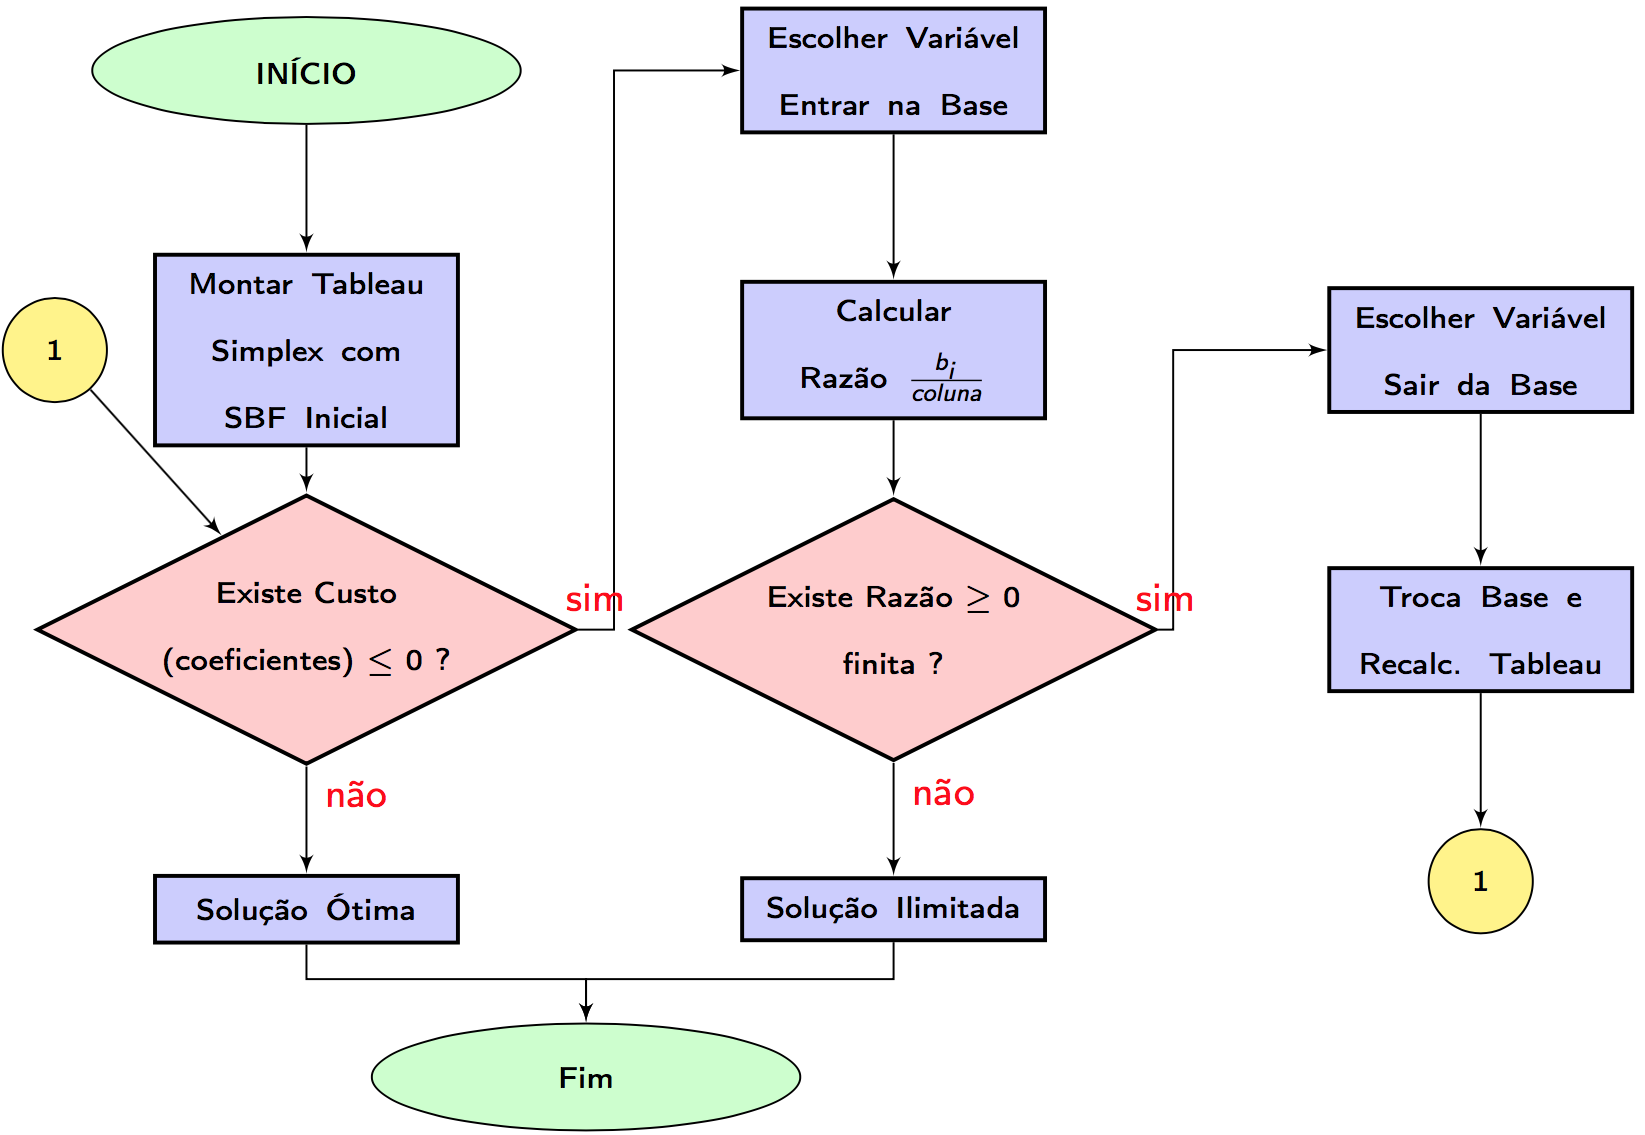
\includegraphics[width=5.5cm,height=3cm]{Alg_1.png}
			}
			\only<2>
			{
				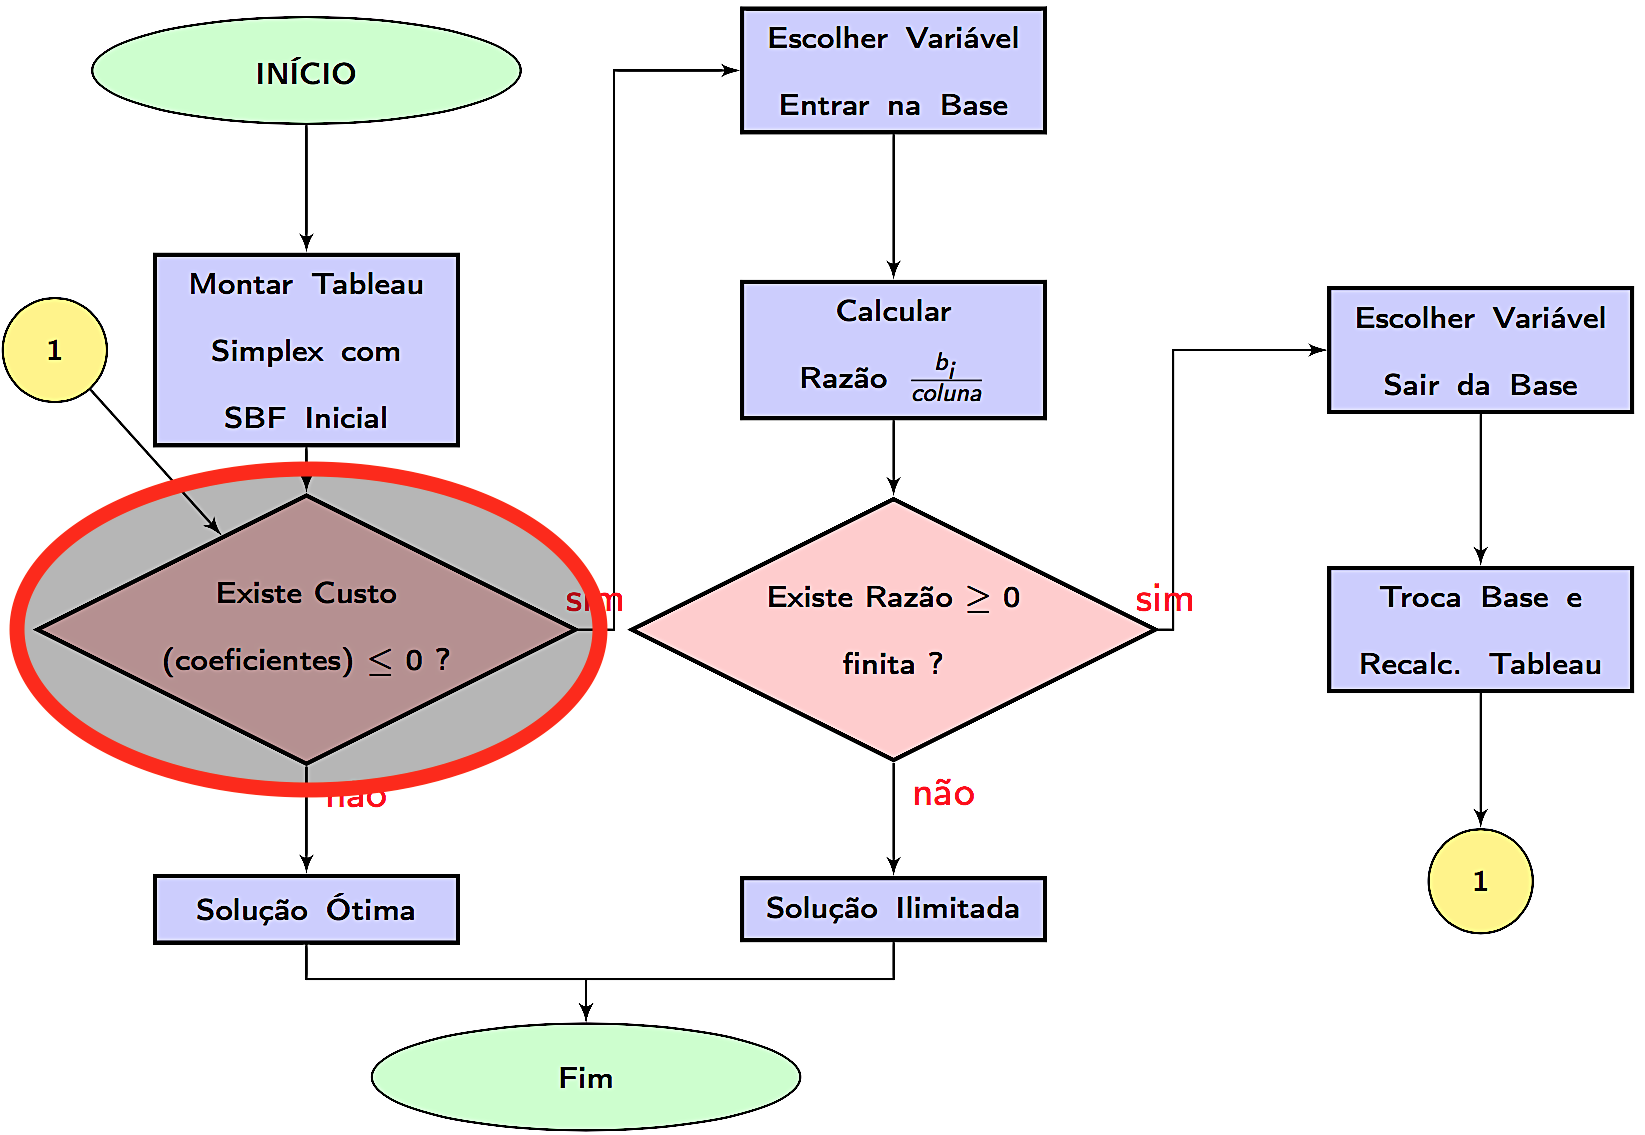
\includegraphics[width=5.5cm,height=3cm]{Alg_2.png}
			}
			\only<3>
			{
				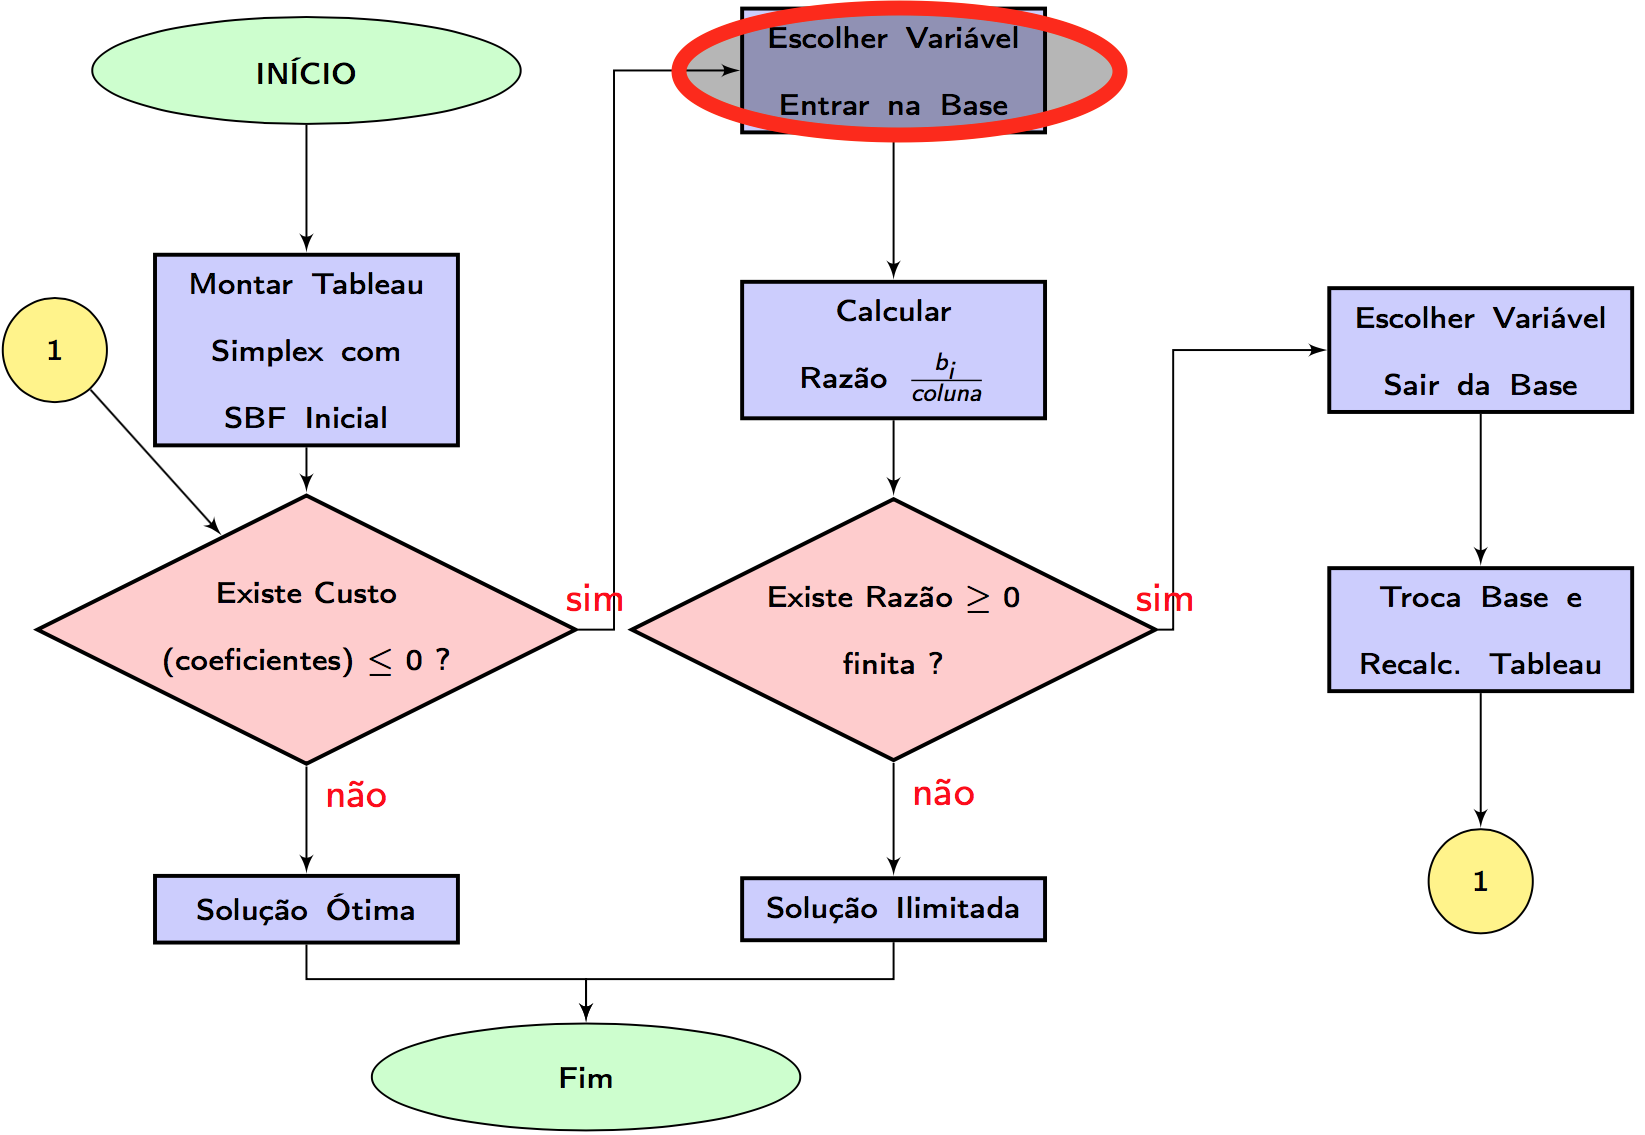
\includegraphics[width=5.5cm,height=3cm]{Alg_3.png}
			}
			\only<4>
			{
				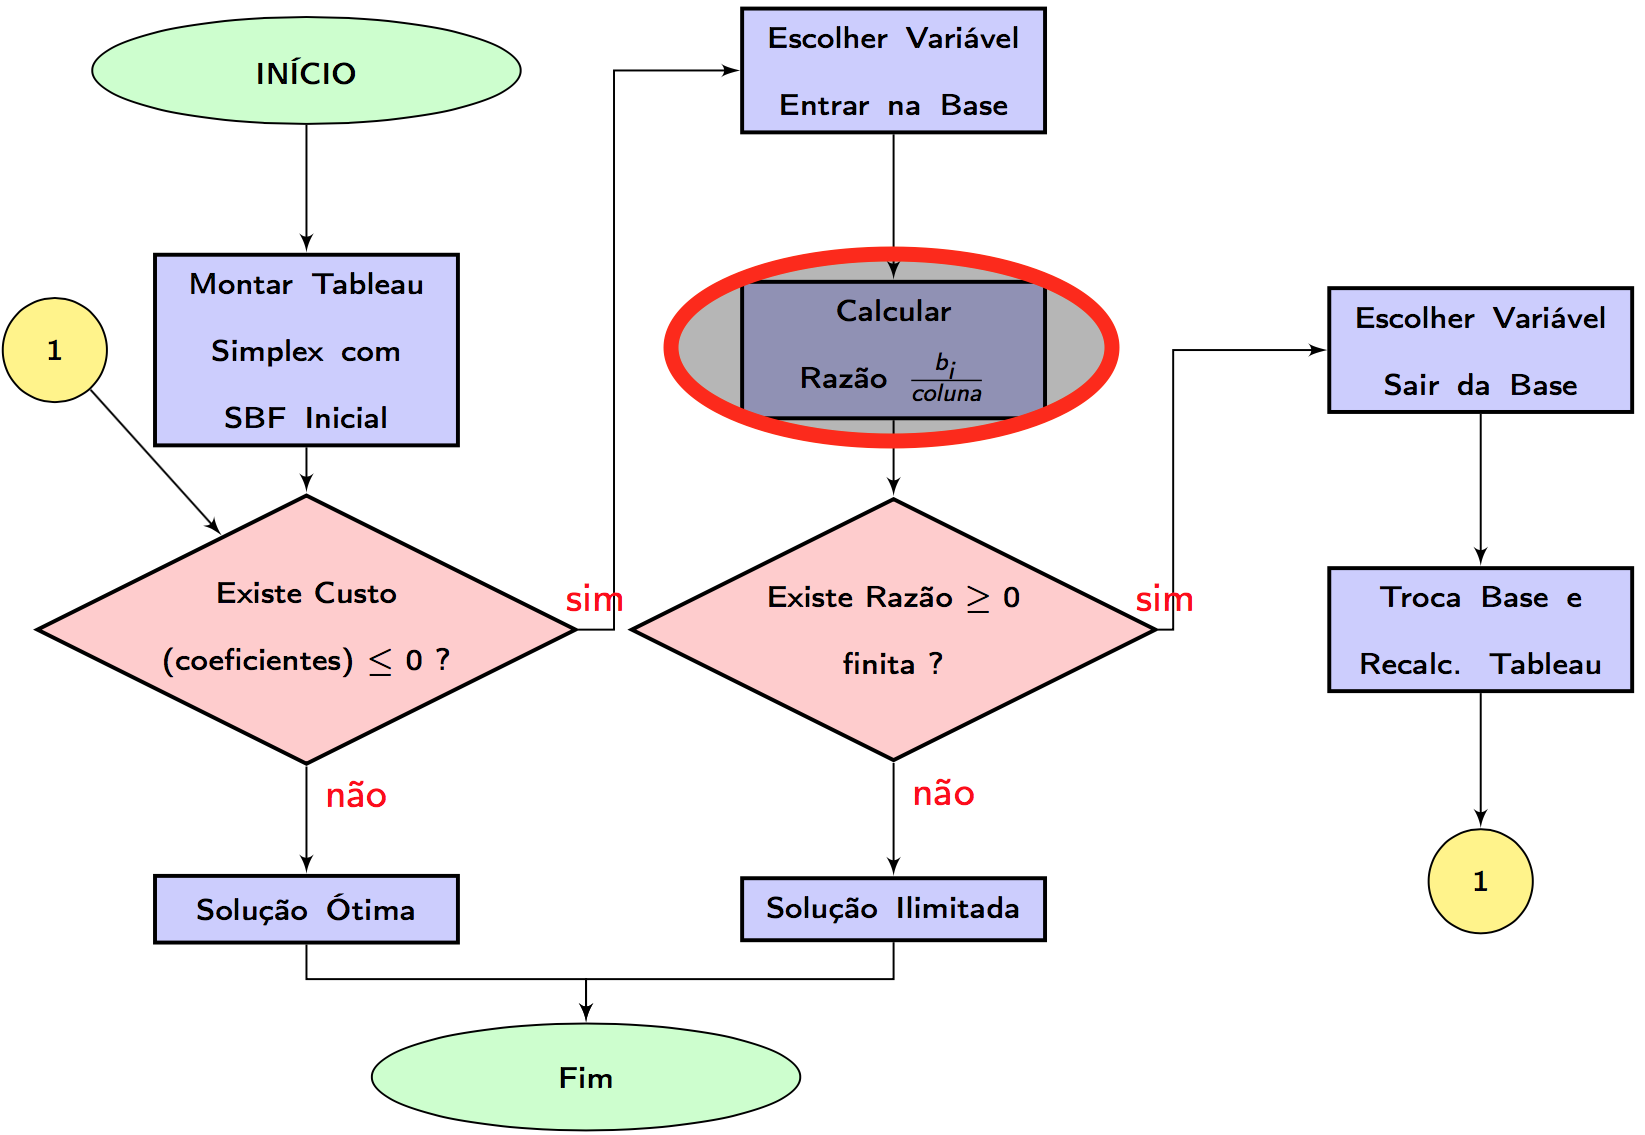
\includegraphics[width=5.5cm,height=3cm]{Alg_4.png}
			}
			\only<5>
			{
				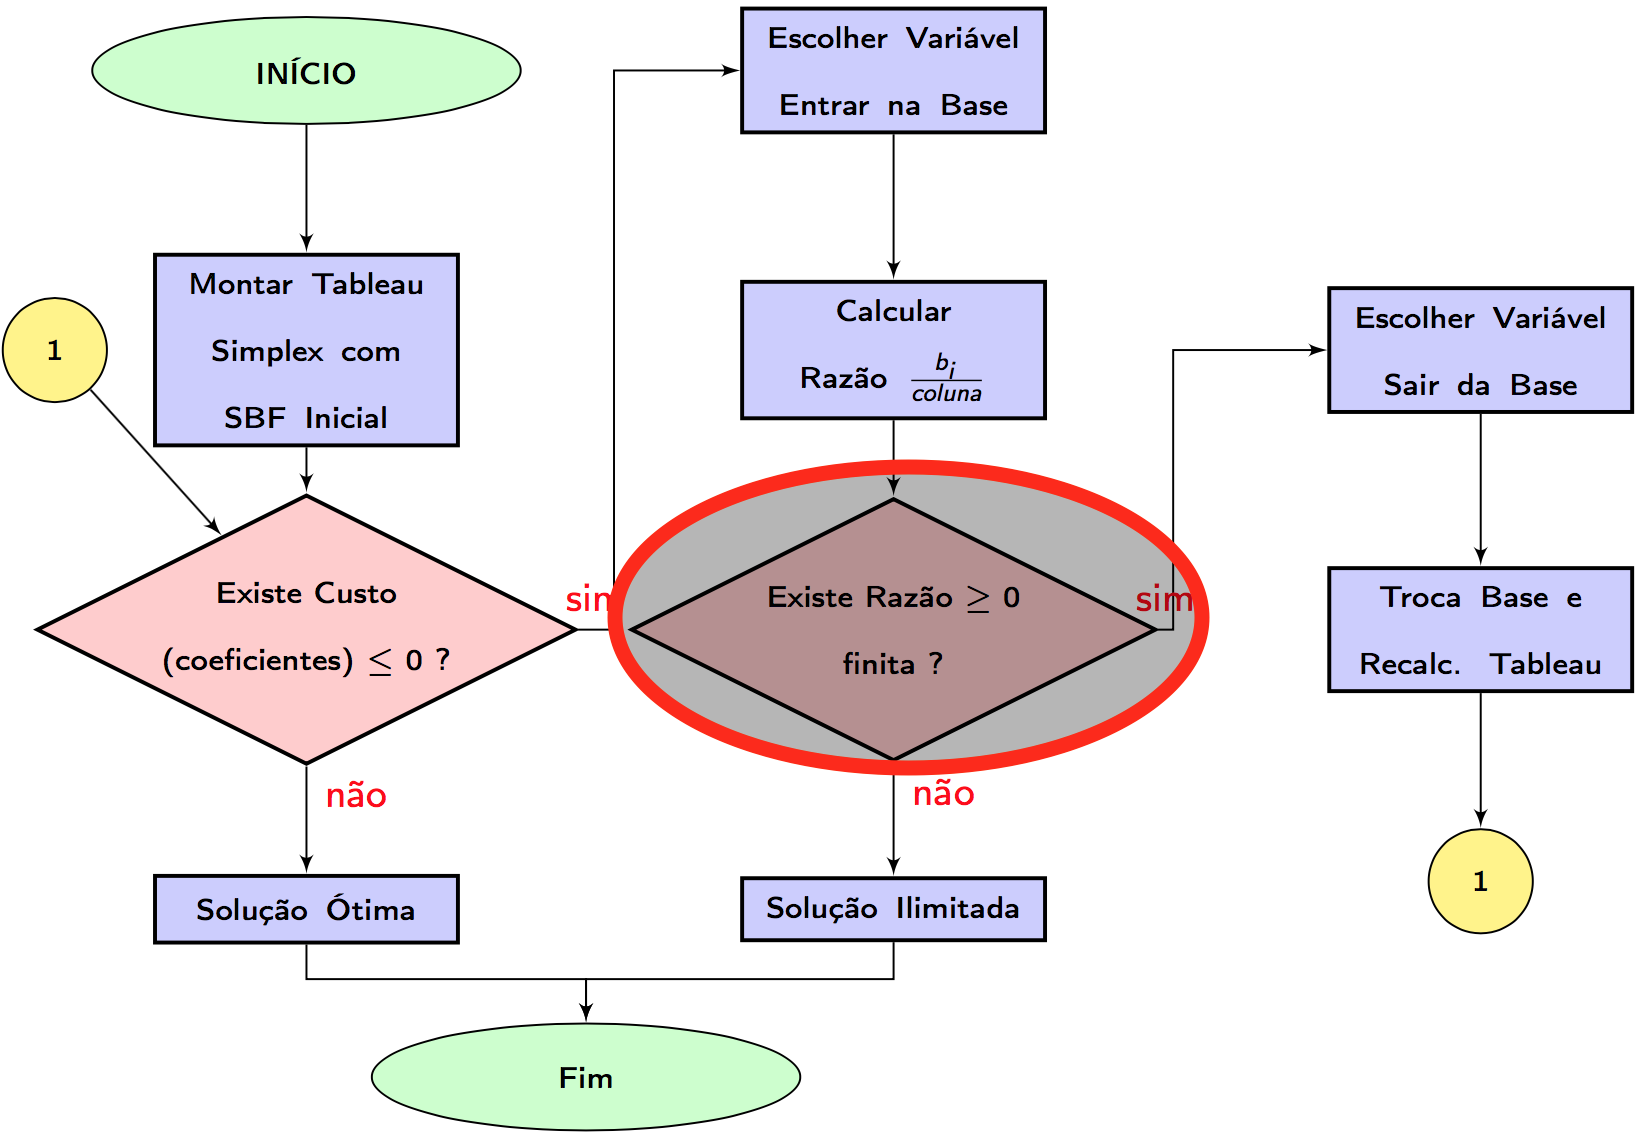
\includegraphics[width=5.5cm,height=3cm]{Alg_5.png}
			}
			\only<6>
			{
				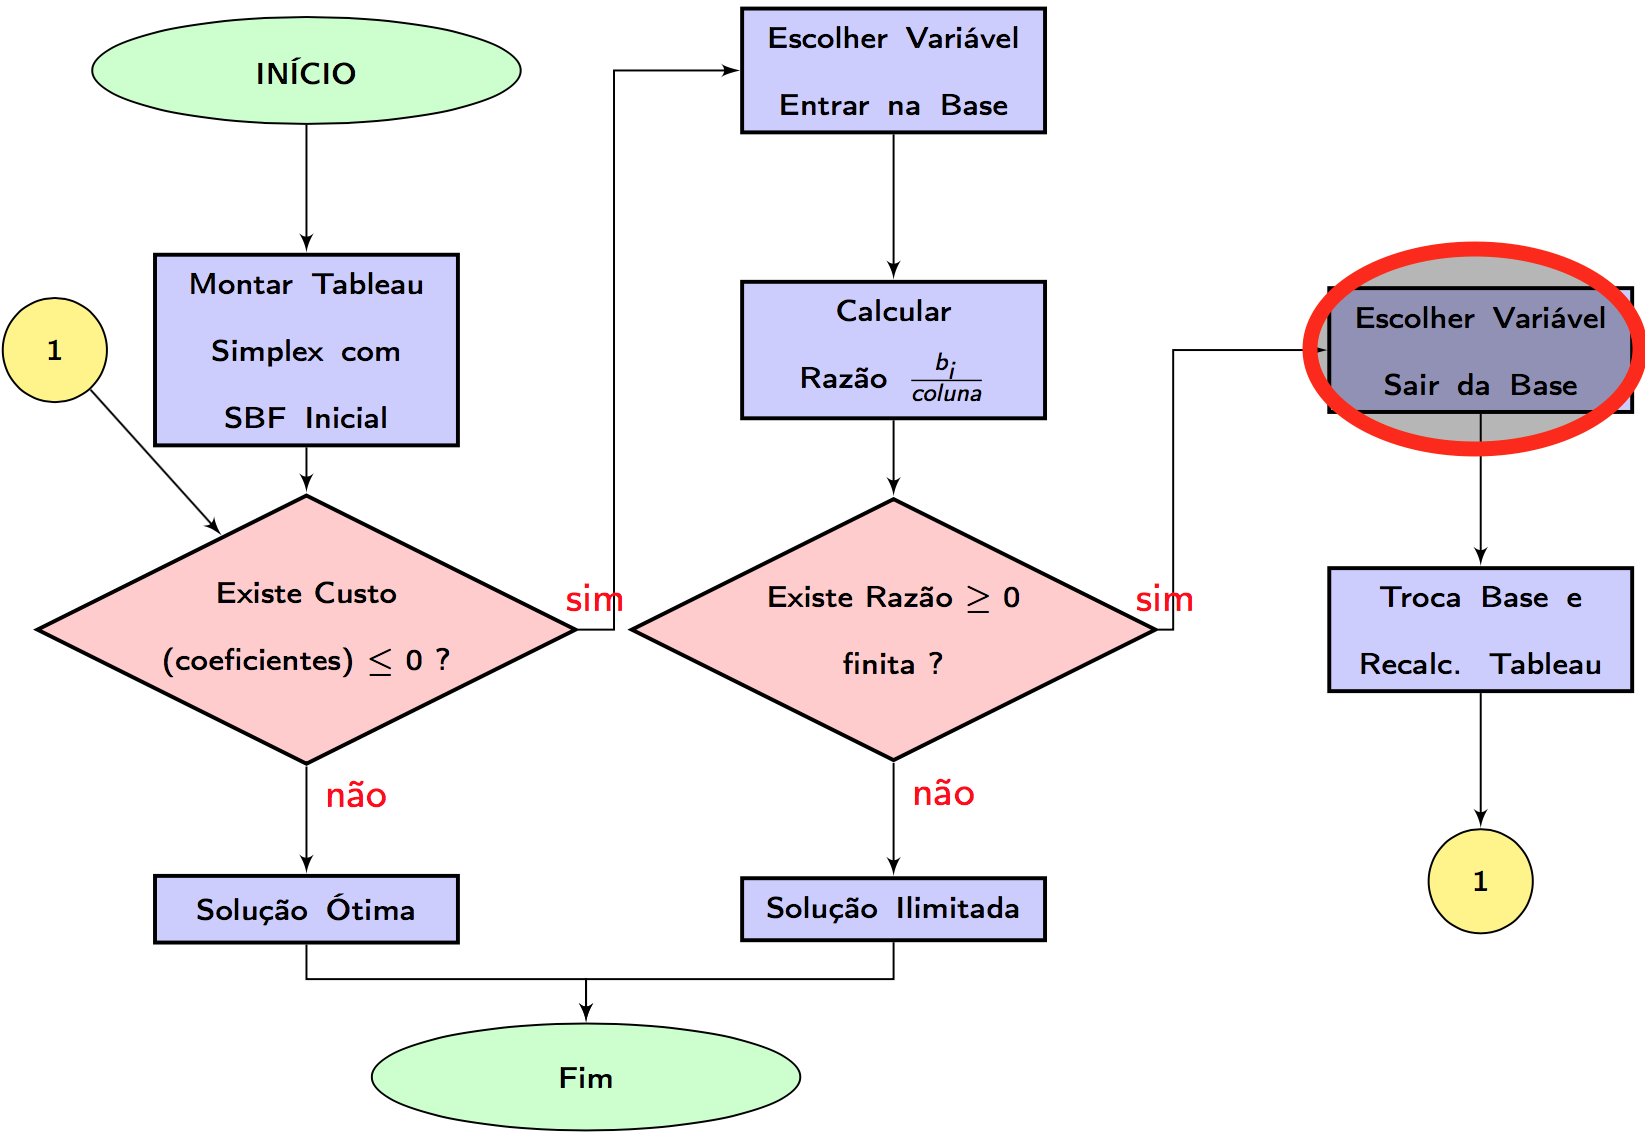
\includegraphics[width=5.5cm,height=3cm]{Alg_6.png}
			}
			\only<7-8>
			{
				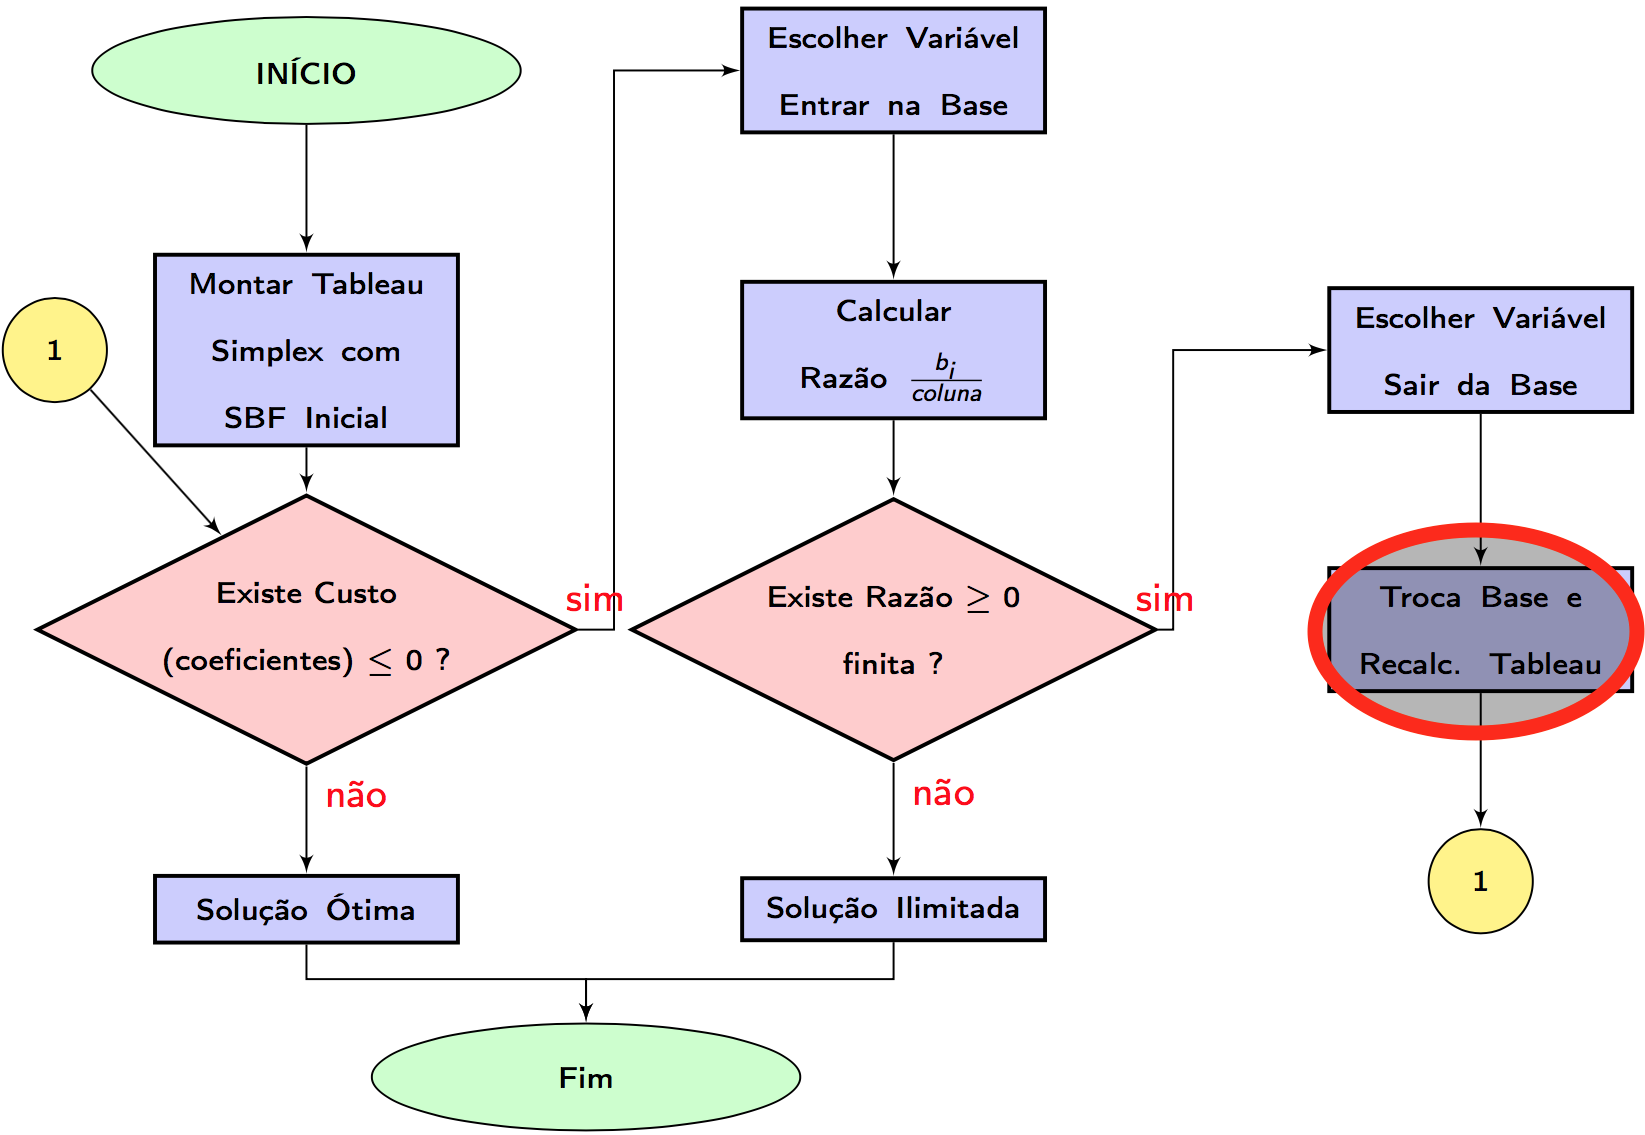
\includegraphics[width=5.5cm,height=3cm]{Alg_7.png}
			}
			\only<9>
			{
				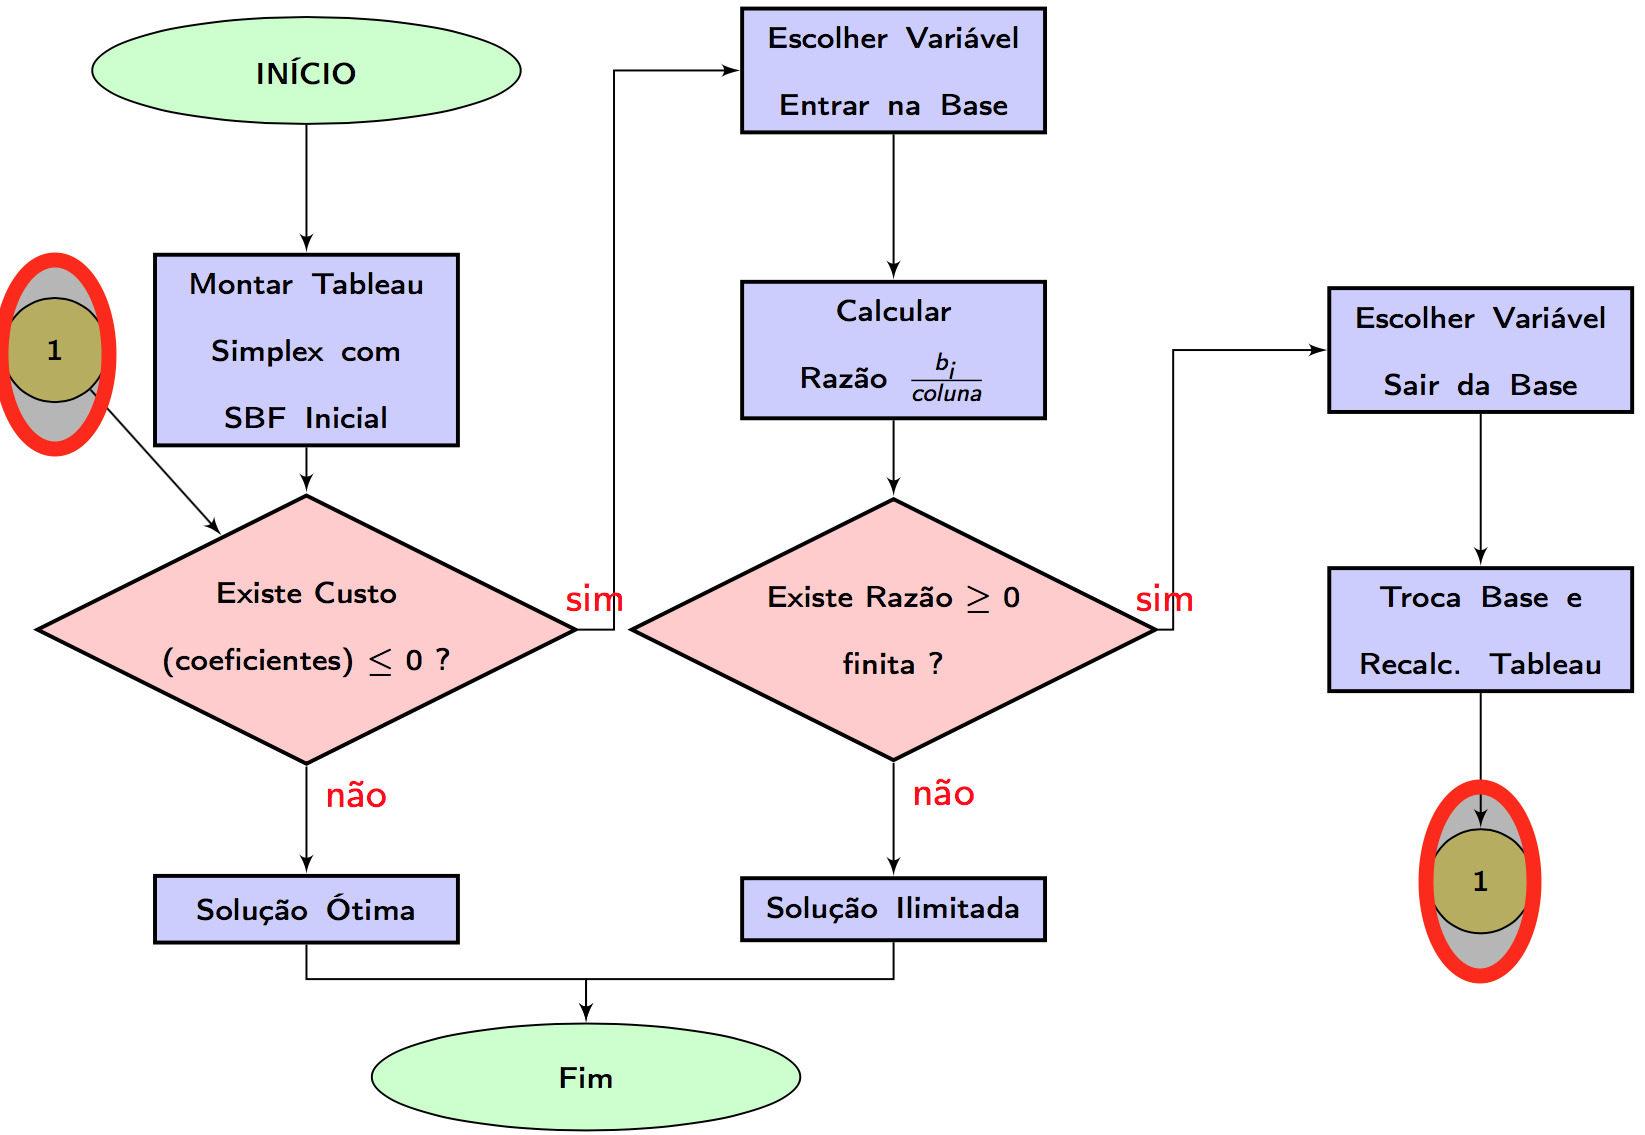
\includegraphics[width=5.5cm,height=3cm]{Alg_9.png}
			}
			\only<10>
			{
				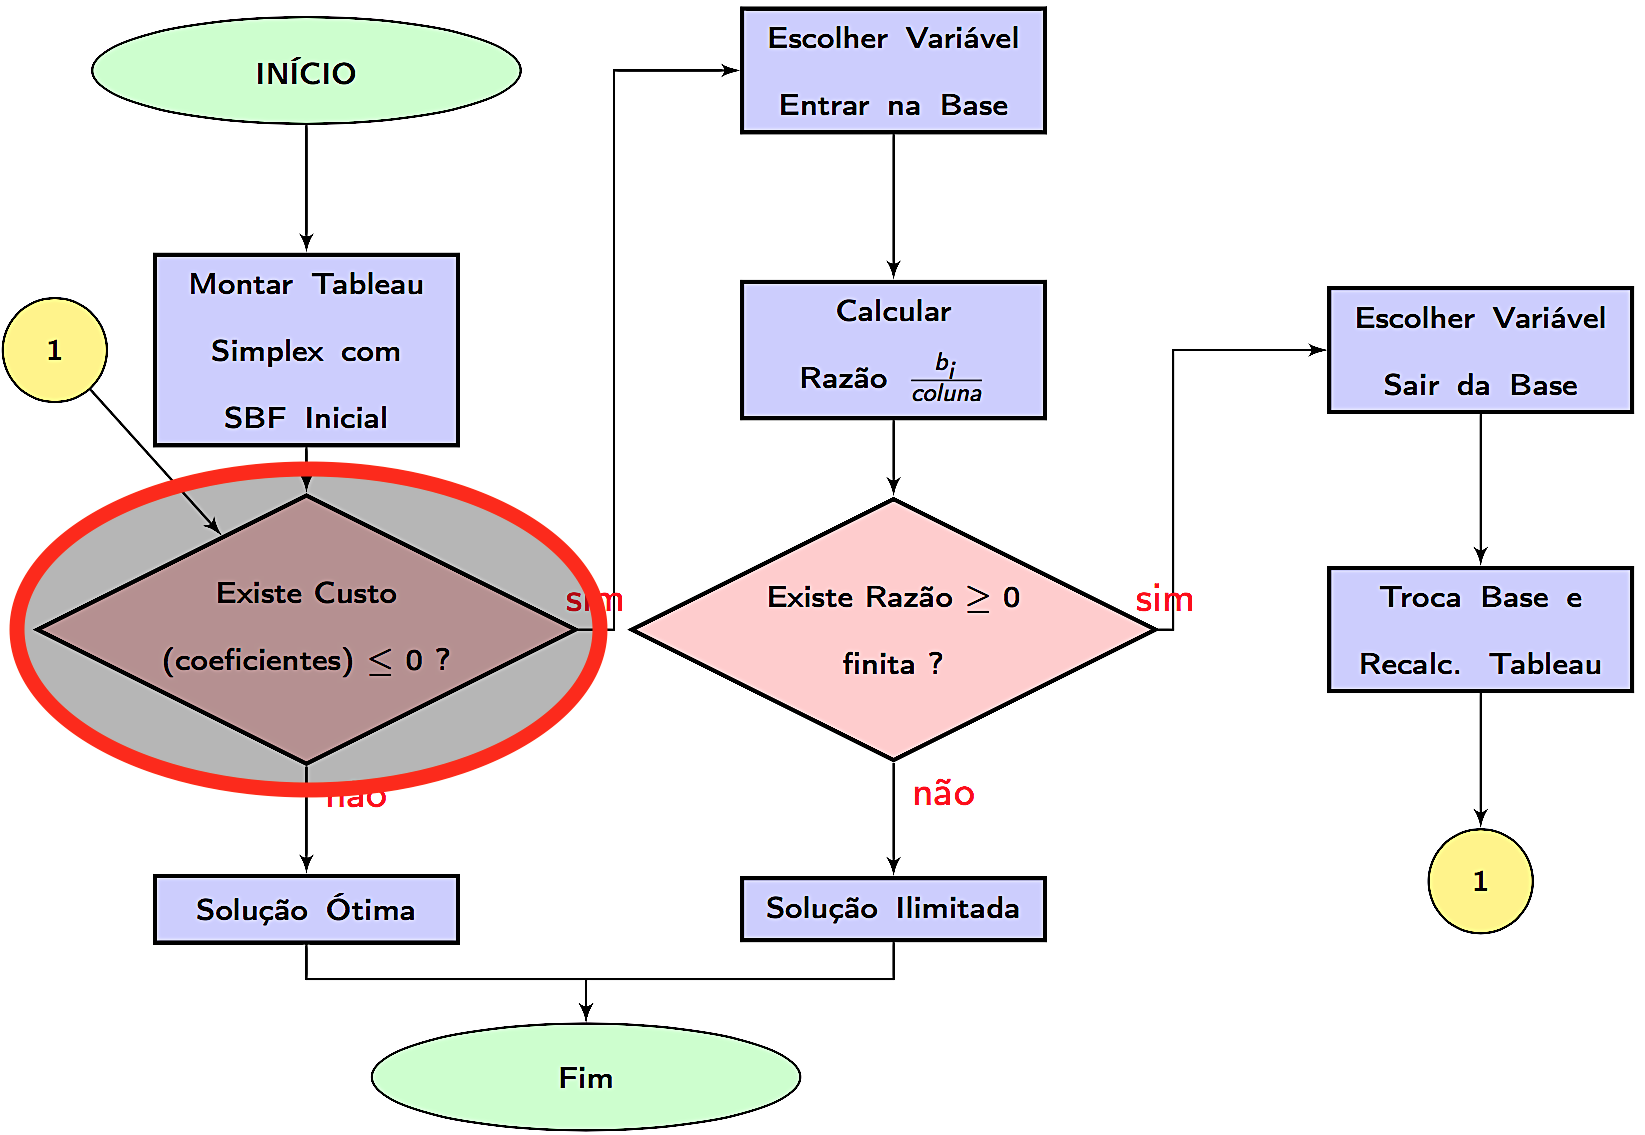
\includegraphics[width=5.5cm,height=3cm]{Alg_2.png}
			}
			\only<11>
			{
				\includegraphics[width=5.5cm,height=3cm]{Alg_3.png}
			}
			\only<12>
			{
				\includegraphics[width=5.5cm,height=3cm]{Alg_4.png}
			}
			\only<13>
			{
				\includegraphics[width=5.5cm,height=3cm]{Alg_5.png}
			}
			\only<14>
			{
				\includegraphics[width=5.5cm,height=3cm]{Alg_6.png}
			}
			\only<15-16>
			{
				\includegraphics[width=5.5cm,height=3cm]{Alg_7.png}
			}
			\only<17>
			{
				\includegraphics[width=5.5cm,height=3cm]{Alg_9.png}
			}
			\only<18>
			{
				\includegraphics[width=5.5cm,height=3cm]{Alg_2.png}
			}
			\only<19-20>
			{
				\includegraphics[width=5.5cm,height=3cm]{Alg_8.png}
			}
		\end{column}
	\end{columns}
\end{frame}


\subsection{Problema de Minimização}
\begin{frame}
	\only<1>
	{
		\frametitle{Fluxograma Tableau Simplex - \color{pink!100} MAXIMIZAÇÃO}
	}
	\only<2>
	{
		\frametitle{Fluxograma Tableau Simplex - \color{cyan!100} MINIMIZAÇÃO}
	}


	\centering
	\only<1>
	{
	\begin{tikzpicture} [
							auto, node distance = 2cm,
							decisao/.style = { diamond, draw, shape aspect=2, thick, fill=red!20,
							                   text width=6em, text badly centered,
							                   inner sep=1pt},
							bloco/.style   = { rectangle, draw, thick, fill=blue!20, 
												text width=5em, text centered,
							                   minimum height=1em },
							bloco2/.style   = { rectangle, draw, thick, fill=blue!20, 
												text width=5em, text centered,
							                   minimum height=1em, node distance = 4.2cm },
							extremo/.style  = { ellipse, draw, fill=green!20,
							                   text width=5em, text centered,
							                   minimum height=2em },	
							line/.style   = { draw, -latex' },
							goto/.style = {circle, draw, fill=yellow!60, text width=1em,
										   text centered, node distance = 1.8cm},
						    bullet/.style = {rectangle, draw, thick, fill=red!80, 
						    				text width=9em, text centered,
						    				minimum height=1em},
						]

	
		\node [extremo] (inic) {\tiny INÍCIO}; 
		
		\node [bloco, below of = inic] (sbfi) {\tiny Montar Tableau Simplex com SBF Inicial};
		\path [line] (inic) -- (sbfi); 
		
		\node [decisao, below of = sbfi] (conv) {\tiny Existe Custo (coeficientes) $<$ 0 ?} ;
		\path [line] (sbfi) -- (conv); 
		
		\node[bloco, below of = conv] (otimo) {\tiny Solução Ótima};
		\path [line] (conv) -- node [near start] {\scriptsize \color{red} não} (otimo); 
	    \node [extremo] at (2,-7.2) (fim) {\tiny Fim};	
	    \path [line] (otimo) |- (2,-6.5) -- (fim); 

		\node[bloco2, right of = inic] (escolhe) {\tiny Escolher Variável Entrar na Base};
		\path [line] (conv) -| (2.2, 0) node [near start] {\scriptsize \color{red} sim} -- (escolhe); 
		
		\node[bloco, below of = escolhe] (razao) {\tiny Calcular Razão $ \frac{b_i}{coluna}$};
		\path [line] (escolhe) -- (razao); 

		\node [decisao, below of = razao] (finito) {\tiny Existe Razão $\ge 0$ finita ?} ;
		\path [line] (razao) -- (finito); 
		
		\node[bloco, below of = finito] (ilimit) {\tiny Solução Ilimitada};
		\path [line] (finito) -- node [near start] {\scriptsize \color{red} não} (ilimit); 
		\path [line] (ilimit) |- (2,-6.5) -- (fim); 

		\node[bloco2, right of = razao] (saibase) {\tiny Escolher Variável Sair da Base};
		\path [line] (finito) -| (6.2, -2) node [near start] {\scriptsize \color{red} sim} -- (saibase);
		
		\node[bloco, below of = saibase] (swap) {\tiny Troca Base e Recalc. Tableau};
		\path[line] (saibase) -- (swap); 
		
		\node[goto, below of = swap] (pula_a) {\tiny 1};
		\node[goto, left of = sbfi] (pula_b) {\tiny 1};
		\path[line] (pula_b) -- (conv);
		\path[line] (swap) -- (pula_a); 
		
		\node[bullet] at (7.5,-0.2) (obs1) {\tiny Coef mais negativo FOB};
		\path[line] (obs1) -- (escolhe);

		\node[bullet] at (7.7,-1) (obs2) {\tiny Menor Razão Positiva};
		\path[line] (obs2) -- (saibase);
		
	\end{tikzpicture}	
	}

	\only<2>
	{
	\begin{tikzpicture} [
							auto, node distance = 2cm,
							decisao/.style = { diamond, draw, shape aspect=2, thick, fill=red!20,
							                   text width=6em, text badly centered,
							                   inner sep=1pt},
							bloco/.style   = { rectangle, draw, thick, fill=blue!20, 
												text width=5em, text centered,
							                   minimum height=1em },
							bloco2/.style   = { rectangle, draw, thick, fill=blue!20, 
												text width=5em, text centered,
							                   minimum height=1em, node distance = 4.2cm },
							extremo/.style  = { ellipse, draw, fill=green!20,
							                   text width=5em, text centered,
							                   minimum height=2em },	
							line/.style   = { draw, -latex' },
							goto/.style = {circle, draw, fill=yellow!60, text width=1em,
										   text centered, node distance = 1.8cm},
						    bullet/.style = {rectangle, draw, thick, fill=red!80, 
						    				text width=9em, text centered,
						    				minimum height=1em},
							decisao2/.style = { diamond, draw, shape aspect=2, thick, fill=cyan!80,
							                   text width=6em, text badly centered,
							                   inner sep=1pt},
						    bullet2/.style = {rectangle, draw, thick, fill=cyan!80, 
						    				text width=9em, text centered,
						    				minimum height=1em},
						]

	
		\node [extremo] (inic) {\tiny INÍCIO}; 
		
		\node [bloco, below of = inic] (sbfi) {\tiny Montar Tableau Simplex com SBF Inicial};
		\path [line] (inic) -- (sbfi); 
		
		\node [decisao2, below of = sbfi] (conv) {\tiny Existe Custo (coeficientes) $>$ 0 ?} ;
		\path [line] (sbfi) -- (conv); 
		
		\node[bloco, below of = conv] (otimo) {\tiny Solução Ótima};
		\path [line] (conv) -- node [near start] {\scriptsize \color{red} não} (otimo); 
	    \node [extremo] at (2,-7.2) (fim) {\tiny Fim};	
	    \path [line] (otimo) |- (2,-6.5) -- (fim); 

		\node[bloco2, right of = inic] (escolhe) {\tiny Escolher Variável Entrar na Base};
		\path [line] (conv) -| (2.2, 0) node [near start] {\scriptsize \color{red} sim} -- (escolhe); 
		
		\node[bloco, below of = escolhe] (razao) {\tiny Calcular Razão $ \frac{b_i}{coluna}$};
		\path [line] (escolhe) -- (razao); 

		\node [decisao, below of = razao] (finito) {\tiny Existe Razão $\ge 0$ finita ?} ;
		\path [line] (razao) -- (finito); 
		
		\node[bloco, below of = finito] (ilimit) {\tiny Solução Ilimitada};
		\path [line] (finito) -- node [near start] {\scriptsize \color{red} não} (ilimit); 
		\path [line] (ilimit) |- (2,-6.5) -- (fim); 

		\node[bloco2, right of = razao] (saibase) {\tiny Escolher Variável Sair da Base};
		\path [line] (finito) -| (6.2, -2) node [near start] {\scriptsize \color{red} sim} -- (saibase);
		
		\node[bloco, below of = saibase] (swap) {\tiny Troca Base e Recalc. Tableau};
		\path[line] (saibase) -- (swap); 
		
		\node[goto, below of = swap] (pula_a) {\tiny 1};
		\node[goto, left of = sbfi] (pula_b) {\tiny 1};
		\path[line] (pula_b) -- (conv);
		\path[line] (swap) -- (pula_a); 
		
		\node[bullet2] at (7.5,-0.2) (obs1) {\tiny Coef mais positivo FOB};
		\path[line] (obs1) -- (escolhe);

		\node[bullet] at (7.7,-1) (obs2) {\tiny Menor Razão Positiva};
		\path[line] (obs2) -- (saibase);
		
	\end{tikzpicture}	
	}


\end{frame}

\subsection{Exemplo Minimização}

\begin{frame}
	\frametitle{Exemplo Minimização}
	\begin{block}{Utilize o Tableau Simplex para resolver o seguinte problema de programação linear:}
		\begin{equation*}
			\begin{matrix}
				\min Z = x_1 + x_2 - 4x_3 \\
				\text{Sujeito à:} \\
				x_1 + x_2 + 2x_3 \le 9 \\
				x_2 + x_2 - x_3 \le 2 \\
				-x_1 + x_2 + x_3 \le 4 \\
				x_1, x_2, x_3 \ge 0 \\
			\end{matrix}
		\end{equation*}
	\end{block}
\end{frame}

\begin{frame}
	\frametitle{Exemplo Minimização}
	\begin{columns}
		\begin{column}{0.3\textwidth}
			\only<1>
			{
				\includegraphics[width=3cm,height=3cm]{number_1.jpg}
			}
			\only<2>
			{
				\includegraphics[width=3cm,height=3cm]{number_2.jpg}
			}
			\only<3>
			{
				\includegraphics[width=3cm,height=3cm]{number_3.jpg}
			}
			\only<4>
			{
				\includegraphics[width=3cm,height=3cm]{number_4.jpg}
			}
		\end{column}
 		\begin{column}{0.7\textwidth}
	 		\only<1>
	 		{	
		 		\begin{block}{Reescrever a expressão da FOB}
					\begin{equation*}
						\begin{matrix}
							\min { \color{red}Z - x_1 - x_2 + 4x_3 = 0} \\
							\text{Sujeito à:} \\
							x_1 + x_2 + 2x_3 \le 9 \\
							x_2 + x_2 - x_3 \le 2 \\
							-x_1 + x_2 + x_3 \le 4 \\
							x_1, x_2, x_3 \ge 0 \\
						\end{matrix}
					\end{equation*}
		 		\end{block}
	 		}
	 		\only<2>
	 		{	
		 		\begin{block}{Problema na Forma Padrão}
					\begin{equation*}
						\begin{matrix}
							\min { \color{red}Z - x_1 - x_2 + 4x_3 = 0} \\
							\text{Sujeito à:} \\
							\begin{matrix}
								x_1 + x_2 + 2x_3 & \cellcolor{red!50}+x_4 &  &  & = 9 \\
								x_2 + x_2 - x_3  & & \cellcolor{red!50}+x_5  &  & = 2 \\
								-x_1 + x_2 + x_3 & & & \cellcolor{red!50}+x_6   & = 4 \\
							\end{matrix} \\
							x_1, x_2, x_3, {\color{red} x_4, x_5, x_6} \ge 0 \\
						\end{matrix}
					\end{equation*}
		 		\end{block}
	 		}
	 		\only<3>
	 		{
		 		\begin{block}{Achar SBF Inicial}
			 		\begin{equation*}
							\text{VNB} \left\{\begin{matrix}
							x_1 = 0 \\ 
							x_2 = 0 \\
							x_3 = 0 \\ 
							\end{matrix}\right.
			 		\end{equation*}

			 		\begin{equation*}
							\text{VB} \left\{\begin{matrix}
							x_4 = 9 \\ 
							x_5 = 2 \\
							x_6 = 4 \\ 
							\end{matrix}\right.
			 		\end{equation*}
		 		\end{block}
	 		}
	 		\only<4>
	 		{
		 		\begin{block}{Montar o Tableau Simplex}
		 			\begin{table}
		 				\begin{tabular}{c c c c c c c c c}
							& \cellcolor{blue!80} \color{white} $ \scriptstyle z$
							& \cellcolor{blue!80} \color{white} $ \scriptstyle x_1$ 
							& \cellcolor{blue!80} \color{white} $ \scriptstyle x_2$
							& \cellcolor{blue!80} \color{white} $ \scriptstyle x_3$
							& \cellcolor{blue!80} \color{red} $ \scriptstyle x_4$
							& \cellcolor{blue!80} \color{red} $ \scriptstyle x_5$
							& \cellcolor{blue!80} \color{red} $ \scriptstyle x_6$ 
							& \cellcolor{blue!80} \color{white} $ \scriptstyle b$ \\
							\cellcolor{blue!80} \color{red} $ \scriptstyle x_4$
							& \cellcolor{yellow!60}  $ \scriptstyle 0$
							& \cellcolor{yellow!60}  $ \scriptstyle 1$ 
							& \cellcolor{yellow!60}  $ \scriptstyle 1$
							& \cellcolor{yellow!60}  $ \scriptstyle 2$
							& \cellcolor{yellow!60}  $ \scriptstyle 1$
							& \cellcolor{yellow!60}  $ \scriptstyle 0$
							& \cellcolor{yellow!60}  $ \scriptstyle 0$ 
							& \cellcolor{yellow!60}  $ \scriptstyle 9$ \\ 
							\cellcolor{blue!80} \color{red} $ \scriptstyle x_5$  
							& \cellcolor{yellow!60}  $ \scriptstyle 0$
							& \cellcolor{yellow!60}  $ \scriptstyle 1$ 
							& \cellcolor{yellow!60}  $ \scriptstyle 1$
							& \cellcolor{yellow!60}  $ \scriptstyle -1$
							& \cellcolor{yellow!60}  $ \scriptstyle 0$
							& \cellcolor{yellow!60}  $ \scriptstyle 1$
							& \cellcolor{yellow!60}  $ \scriptstyle 0$ 
							& \cellcolor{yellow!60}  $ \scriptstyle 2$ \\
							\cellcolor{blue!80} \color{red} $ \scriptstyle x_6$
							& \cellcolor{yellow!60}  $ \scriptstyle 0$
							& \cellcolor{yellow!60}  $ \scriptstyle -1$ 
							& \cellcolor{yellow!60}  $ \scriptstyle 1$
							& \cellcolor{yellow!60}  $ \scriptstyle 1$
							& \cellcolor{yellow!60}  $ \scriptstyle 0$
							& \cellcolor{yellow!60}  $ \scriptstyle 0$
							& \cellcolor{yellow!60}  $ \scriptstyle 1$ 
							& \cellcolor{yellow!60}  $ \scriptstyle 4$ \\
							\cellcolor{blue!80} \color{white} $ \scriptstyle z$
							& \cellcolor{yellow!60}  $ \scriptstyle 1$
							& \cellcolor{yellow!60}  $ \scriptstyle -1$ 
							& \cellcolor{yellow!60}  $ \scriptstyle -1$
							& \cellcolor{yellow!60}  $ \scriptstyle 4$
							& \cellcolor{yellow!60}  $ \scriptstyle 0$
							& \cellcolor{yellow!60}  $ \scriptstyle 0$
							& \cellcolor{yellow!60}  $ \scriptstyle 0$ 
							& \cellcolor{yellow!60}  $ \scriptstyle 0$ \\
		 				\end{tabular}
		 			\end{table}
		 		\end{block}
	 		}
 		\end{column}
	\end{columns}
\end{frame}

\begin{frame}
	\only<1-9>
	{
	\frametitle{Exemplo Minimização - $1^a$ Interação}
	}
	\only<10-18>
	{
		\frametitle{Exemplo Minimização - $2^a$ Interação}
	}
	\only<19->
	{
		\frametitle{Exemplo Minimização - $3^a$ Interação}
	}


	\only<1>
	{
	\begin{table}
		\begin{tabular}{c c c c c c c c c c c c}
			& \cellcolor{blue!80} \color{white} $ \scriptstyle z$
			& \cellcolor{blue!80} \color{white} $ \scriptstyle x_1$ 
			& \cellcolor{blue!80} \color{white} $ \scriptstyle x_2$
			& \cellcolor{blue!80} \color{white} $ \scriptstyle x_3$
			& \cellcolor{blue!80} \color{red} $ \scriptstyle x_4$
			& \cellcolor{blue!80} \color{red} $ \scriptstyle x_5$
			& \cellcolor{blue!80} \color{red} $ \scriptstyle x_6$ 
			& \cellcolor{blue!80} \color{white} $ \scriptstyle b$ \\
			\cellcolor{blue!80} \color{red} $ \scriptstyle x_4$
			& \cellcolor{yellow!60}  $ \scriptstyle 0$
			& \cellcolor{yellow!60}  $ \scriptstyle 1$ 
			& \cellcolor{yellow!60}  $ \scriptstyle 1$
			& \cellcolor{yellow!60}  $ \scriptstyle 2$
			& \cellcolor{yellow!60}  $ \scriptstyle 1$
			& \cellcolor{yellow!60}  $ \scriptstyle 0$
			& \cellcolor{yellow!60}  $ \scriptstyle 0$ 
			& \cellcolor{yellow!60}  $ \scriptstyle 9$ \\ 
			\cellcolor{blue!80} \color{red} $ \scriptstyle x_5$  
			& \cellcolor{yellow!60}  $ \scriptstyle 0$
			& \cellcolor{yellow!60}  $ \scriptstyle 1$ 
			& \cellcolor{yellow!60}  $ \scriptstyle 1$
			& \cellcolor{yellow!60}  $ \scriptstyle -1$
			& \cellcolor{yellow!60}  $ \scriptstyle 0$
			& \cellcolor{yellow!60}  $ \scriptstyle 1$
			& \cellcolor{yellow!60}  $ \scriptstyle 0$ 
			& \cellcolor{yellow!60}  $ \scriptstyle 2$ \\
			\cellcolor{blue!80} \color{red} $ \scriptstyle x_6$
			& \cellcolor{yellow!60}  $ \scriptstyle 0$
			& \cellcolor{yellow!60}  $ \scriptstyle -1$ 
			& \cellcolor{yellow!60}  $ \scriptstyle 1$
			& \cellcolor{yellow!60}  $ \scriptstyle 1$
			& \cellcolor{yellow!60}  $ \scriptstyle 0$
			& \cellcolor{yellow!60}  $ \scriptstyle 0$
			& \cellcolor{yellow!60}  $ \scriptstyle 1$ 
			& \cellcolor{yellow!60}  $ \scriptstyle 4$ \\
			\cellcolor{blue!80} \color{white} $ \scriptstyle z$
			& \cellcolor{yellow!60}  $ \scriptstyle 1$
			& \cellcolor{yellow!60}  $ \scriptstyle -1$ 
			& \cellcolor{yellow!60}  $ \scriptstyle -1$
			& \cellcolor{yellow!60}  $ \scriptstyle 4$
			& \cellcolor{yellow!60}  $ \scriptstyle 0$
			& \cellcolor{yellow!60}  $ \scriptstyle 0$
			& \cellcolor{yellow!60}  $ \scriptstyle 0$ 
			& \cellcolor{yellow!60}  $ \scriptstyle 0$ \\
		\end{tabular}
	\end{table}
	}	
	\only<2>
	{
		\begin{table}
			\begin{tabular}{c c c c c c c c c c c c}
				& \cellcolor{blue!80} \color{white} $ \scriptstyle z$
				& \cellcolor{blue!80} \color{white} $ \scriptstyle x_1$ 
				& \cellcolor{blue!80} \color{white} $ \scriptstyle x_2$
				& \cellcolor{blue!80} \color{white} $ \scriptstyle x_3$
				& \cellcolor{blue!80} \color{red} $ \scriptstyle x_4$
				& \cellcolor{blue!80} \color{red} $ \scriptstyle x_5$
				& \cellcolor{blue!80} \color{red} $ \scriptstyle x_6$ 
				& \cellcolor{blue!80} \color{white} $ \scriptstyle b$ \\
				\cellcolor{blue!80} \color{red} $ \scriptstyle x_4$
				& \cellcolor{yellow!60}  $ \scriptstyle 0$
				& \cellcolor{yellow!60}  $ \scriptstyle 1$ 
				& \cellcolor{yellow!60}  $ \scriptstyle 1$
				& \cellcolor{gray!60}  $ \scriptstyle 2$
				& \cellcolor{yellow!60}  $ \scriptstyle 1$
				& \cellcolor{yellow!60}  $ \scriptstyle 0$
				& \cellcolor{yellow!60}  $ \scriptstyle 0$ 
				& \cellcolor{yellow!60}  $ \scriptstyle 9$ \\ 
				\cellcolor{blue!80} \color{red} $ \scriptstyle x_5$  
				& \cellcolor{yellow!60}  $ \scriptstyle 0$
				& \cellcolor{yellow!60}  $ \scriptstyle 1$ 
				& \cellcolor{yellow!60}  $ \scriptstyle 1$
				& \cellcolor{gray!60}  $ \scriptstyle -1$
				& \cellcolor{yellow!60}  $ \scriptstyle 0$
				& \cellcolor{yellow!60}  $ \scriptstyle 1$
				& \cellcolor{yellow!60}  $ \scriptstyle 0$ 
				& \cellcolor{yellow!60}  $ \scriptstyle 2$ \\
				\cellcolor{blue!80} \color{red} $ \scriptstyle x_6$
				& \cellcolor{yellow!60}  $ \scriptstyle 0$
				& \cellcolor{yellow!60}  $ \scriptstyle -1$ 
				& \cellcolor{yellow!60}  $ \scriptstyle 1$
				& \cellcolor{gray!60}  $ \scriptstyle 1$
				& \cellcolor{yellow!60}  $ \scriptstyle 0$
				& \cellcolor{yellow!60}  $ \scriptstyle 0$
				& \cellcolor{yellow!60}  $ \scriptstyle 1$ 
				& \cellcolor{yellow!60}  $ \scriptstyle 4$ \\
				\cellcolor{blue!80} \color{white} $ \scriptstyle z$
				& \cellcolor{yellow!60}  $ \scriptstyle 1$
				& \cellcolor{yellow!60}  $ \scriptstyle -1$ 
				& \cellcolor{yellow!60}  $ \scriptstyle -1$
				& \cellcolor{gray!60}  $ \scriptstyle 4$
				& \cellcolor{yellow!60}  $ \scriptstyle 0$
				& \cellcolor{yellow!60}  $ \scriptstyle 0$
				& \cellcolor{yellow!60}  $ \scriptstyle 0$ 
				& \cellcolor{yellow!60}  $ \scriptstyle 0$ \\
				
				& 
				&  
				& 
				& \includegraphics[width=0.3cm,height=0.3cm]{setacima.jpg}
				& 
				& 
				&  
				&  \\
				
				& 
				&  
				& 
				& \scriptsize Entra 
				& 
				& 
				&  
				&  \\
				
				& 
				&  
				& 
				& \scriptsize Base
				& 
				& 
				&  
				&  \\
			\end{tabular}
		\end{table}
	}
	\only<3>
	{
		\begin{table}
			\begin{tabular}{c c c c c c c c c c c c}
				& \cellcolor{blue!80} \color{white} $ \scriptstyle z$
				& \cellcolor{blue!80} \color{white} $ \scriptstyle x_1$ 
				& \cellcolor{blue!80} \color{white} $ \scriptstyle x_2$
				& \cellcolor{blue!80} \color{white} $ \scriptstyle x_3$
				& \cellcolor{blue!80} \color{red} $ \scriptstyle x_4$
				& \cellcolor{blue!80} \color{red} $ \scriptstyle x_5$
				& \cellcolor{blue!80} \color{red} $ \scriptstyle x_6$ 
				& \cellcolor{blue!80} \color{white} $ \scriptstyle b$ 
				& & & \\
				\cellcolor{blue!80} \color{red} $ \scriptstyle x_4$
				& \cellcolor{yellow!60}  $ \scriptstyle 0$
				& \cellcolor{yellow!60}  $ \scriptstyle 1$ 
				& \cellcolor{yellow!60}  $ \scriptstyle 1$
				& \cellcolor{gray!60}  $ \scriptstyle 2$
				& \cellcolor{yellow!60}  $ \scriptstyle 1$
				& \cellcolor{yellow!60}  $ \scriptstyle 0$
				& \cellcolor{yellow!60}  $ \scriptstyle 0$ 
				& \cellcolor{gray!60}  $ \scriptstyle 9$ 
				& $ \scriptstyle 9 \div 2 = 4,5 $ & \includegraphics[width=0.3cm,height=0.3cm]{setaesquerda.jpg} & \\ 
				\cellcolor{blue!80} \color{red} $ \scriptstyle x_5$  
				& \cellcolor{yellow!60}  $ \scriptstyle 0$
				& \cellcolor{yellow!60}  $ \scriptstyle 1$ 
				& \cellcolor{yellow!60}  $ \scriptstyle 1$
				& \cellcolor{gray!60}  $ \scriptstyle -1$
				& \cellcolor{yellow!60}  $ \scriptstyle 0$
				& \cellcolor{yellow!60}  $ \scriptstyle 1$
				& \cellcolor{yellow!60}  $ \scriptstyle 0$ 
				& \cellcolor{gray!60}  $ \scriptstyle 2$
				& $ \scriptstyle 2 \div (-1) = -2 $ & & \\
				\cellcolor{blue!80} \color{red} $ \scriptstyle x_6$
				& \cellcolor{yellow!60}  $ \scriptstyle 0$
				& \cellcolor{yellow!60}  $ \scriptstyle -1$ 
				& \cellcolor{yellow!60}  $ \scriptstyle 1$
				& \cellcolor{gray!60}  $ \scriptstyle 1$
				& \cellcolor{yellow!60}  $ \scriptstyle 0$
				& \cellcolor{yellow!60}  $ \scriptstyle 0$
				& \cellcolor{yellow!60}  $ \scriptstyle 1$ 
				& \cellcolor{gray!60}  $ \scriptstyle 4$ 
				& $ \scriptstyle 4 \div 1 = 4 $& \includegraphics[width=0.3cm,height=0.3cm]{setaesquerda.jpg} & \\
				\cellcolor{blue!80} \color{white} $ \scriptstyle z$
				& \cellcolor{yellow!60}  $ \scriptstyle 1$
				& \cellcolor{yellow!60}  $ \scriptstyle -1$ 
				& \cellcolor{yellow!60}  $ \scriptstyle -1$
				& \cellcolor{gray!60}  $ \scriptstyle 4$
				& \cellcolor{yellow!60}  $ \scriptstyle 0$
				& \cellcolor{yellow!60}  $ \scriptstyle 0$
				& \cellcolor{yellow!60}  $ \scriptstyle 0$ 
				& \cellcolor{gray!60}  $ \scriptstyle 0$ 
				& & & \\
				
				& 
				&  
				& 
				& \includegraphics[width=0.3cm,height=0.3cm]{setacima.jpg}
				& 
				& 
				&  
				&  
				& & & \\
				
				& 
				&  
				& 
				& \scriptsize Entra 
				& 
				& 
				&  
				&  
				& & & \\
				
				& 
				&  
				& 
				& \scriptsize Base
				& 
				& 
				&  
				&  
				& & & \\
			\end{tabular}
		\end{table}
	}
	\only<4-9>
	{
		\begin{table}
			\begin{tabular}{c c c c c c c c c c c c}
				& \cellcolor{blue!80} \color{white} $ \scriptstyle z$
				& \cellcolor{blue!80} \color{white} $ \scriptstyle x_1$ 
				& \cellcolor{blue!80} \color{white} $ \scriptstyle x_2$
				& \cellcolor{blue!80} \color{white} $ \scriptstyle x_3$
				& \cellcolor{blue!80} \color{red} $ \scriptstyle x_4$
				& \cellcolor{blue!80} \color{red} $ \scriptstyle x_5$
				& \cellcolor{blue!80} \color{red} $ \scriptstyle x_6$ 
				& \cellcolor{blue!80} \color{white} $ \scriptstyle b$ 
				& & & \\
				\cellcolor{blue!80} \color{red} $ \scriptstyle x_4$
				& \cellcolor{yellow!60}  $ \scriptstyle 0$
				& \cellcolor{yellow!60}  $ \scriptstyle 1$ 
				& \cellcolor{yellow!60}  $ \scriptstyle 1$
				& \cellcolor{gray!60}  $ \scriptstyle 2$
				& \cellcolor{yellow!60}  $ \scriptstyle 1$
				& \cellcolor{yellow!60}  $ \scriptstyle 0$
				& \cellcolor{yellow!60}  $ \scriptstyle 0$ 
				& \cellcolor{gray!60}  $ \scriptstyle 9$ 
				& $ \scriptstyle 9 \div 2 = 4,5 $ &  & \\ 
				\cellcolor{blue!80} \color{red} $ \scriptstyle x_5$  
				& \cellcolor{yellow!60}  $ \scriptstyle 0$
				& \cellcolor{yellow!60}  $ \scriptstyle 1$ 
				& \cellcolor{yellow!60}  $ \scriptstyle 1$
				& \cellcolor{gray!60}  $ \scriptstyle -1$
				& \cellcolor{yellow!60}  $ \scriptstyle 0$
				& \cellcolor{yellow!60}  $ \scriptstyle 1$
				& \cellcolor{yellow!60}  $ \scriptstyle 0$ 
				& \cellcolor{gray!60}  $ \scriptstyle 2$
				& $ \scriptstyle 2 \div (-1) = -2 $ & & \\
				\cellcolor{blue!80} \color{red} $ \scriptstyle x_6$
				& \cellcolor{gray!60}  $ \scriptstyle 0$
				& \cellcolor{gray!60}  $ \scriptstyle -1$ 
				& \cellcolor{gray!60}  $ \scriptstyle 1$
				& \cellcolor{red!70}  $ \scriptstyle 1$
				& \cellcolor{gray!60}  $ \scriptstyle 0$
				& \cellcolor{gray!60}  $ \scriptstyle 0$
				& \cellcolor{gray!60}  $ \scriptstyle 1$ 
				& \cellcolor{gray!60}  $ \scriptstyle 4$ 
				& $ \scriptstyle 4 \div 1 = 4 $
				& \includegraphics[width=0.3cm,height=0.3cm]{setaesquerda.jpg} 
				& \scriptsize Sai Base\\
				\cellcolor{blue!80} \color{white} $ \scriptstyle z$
				& \cellcolor{yellow!60}  $ \scriptstyle 1$
				& \cellcolor{yellow!60}  $ \scriptstyle -1$ 
				& \cellcolor{yellow!60}  $ \scriptstyle -1$
				& \cellcolor{gray!60}  $ \scriptstyle 4$
				& \cellcolor{yellow!60}  $ \scriptstyle 0$
				& \cellcolor{yellow!60}  $ \scriptstyle 0$
				& \cellcolor{yellow!60}  $ \scriptstyle 0$ 
				& \cellcolor{gray!60}  $ \scriptstyle 0$ 
				& & & \\
				
				& 
				&  
				& 
				& \includegraphics[width=0.3cm,height=0.3cm]{setacima.jpg}
				& 
				& 
				&  
				&  
				& & & \\
				
				& 
				&  
				& 
				& \scriptsize Entra 
				& 
				& 
				&  
				&  
				& & & \\
				
				& 
				&  
				& 
				& \scriptsize Base
				& 
				& 
				&  
				&  
				& & & \\
			\end{tabular}
		\end{table}
		\begin{itemize}
			\item[] \only<5-9> {Zerar coluna de $X_3$ com exceção da linha referente a $X_6$ que deve assumir o valor unitário (pivô). Para tanto:}
			\item[] \only<6-9> {$ \color{red} \text{Linha}'_1 = \text{Linha}_1 - 2*\text{Linha}_3$}
			\item[] \only<7-9> {$ \color{red} \text{Linha}'_2 = \text{Linha}_2 + 1*\text{Linha}_3$}
			\item[] \only<8-9> {$ \color{red} \text{Linha}'_3 = \text{Linha}_3$}
			\item[] \only<9>   {$ \color{red} \text{Linha}'_4 = \text{Linha}_4 - 4*\text{Linha}_3$}
		\end{itemize}
	}
	
	\only<10>
	{
		\begin{table}
			\begin{tabular}{c c c c c c c c c c c c}
				& \cellcolor{blue!80} \color{white} $ \scriptstyle z$
				& \cellcolor{blue!80} \color{white} $ \scriptstyle x_1$ 
				& \cellcolor{blue!80} \color{white} $ \scriptstyle x_2$
				& \cellcolor{blue!80} \color{red} $ \scriptstyle x_3$
				& \cellcolor{blue!80} \color{red} $ \scriptstyle x_4$
				& \cellcolor{blue!80} \color{red} $ \scriptstyle x_5$
				& \cellcolor{blue!80} \color{white} $ \scriptstyle x_6$ 
				& \cellcolor{blue!80} \color{white} $ \scriptstyle b$ \\
				\cellcolor{blue!80} \color{red} $ \scriptstyle x_4$
				& \cellcolor{yellow!60}  $ \scriptstyle 0$
				& \cellcolor{yellow!60}  $ \scriptstyle 3$ 
				& \cellcolor{yellow!60}  $ \scriptstyle -1$
				& \cellcolor{yellow!60}  $ \scriptstyle 0$
				& \cellcolor{yellow!60}  $ \scriptstyle 1$
				& \cellcolor{yellow!60}  $ \scriptstyle 0$
				& \cellcolor{yellow!60}  $ \scriptstyle -2$ 
				& \cellcolor{yellow!60}  $ \scriptstyle 1$ \\ 
				\cellcolor{blue!80} \color{red} $ \scriptstyle x_5$  
				& \cellcolor{yellow!60}  $ \scriptstyle 0$
				& \cellcolor{yellow!60}  $ \scriptstyle 0$ 
				& \cellcolor{yellow!60}  $ \scriptstyle 2$
				& \cellcolor{yellow!60}  $ \scriptstyle 0$
				& \cellcolor{yellow!60}  $ \scriptstyle 0$
				& \cellcolor{yellow!60}  $ \scriptstyle 1$
				& \cellcolor{yellow!60}  $ \scriptstyle 1$ 
				& \cellcolor{yellow!60}  $ \scriptstyle 6$ \\
				\cellcolor{blue!80} \color{red} $ \scriptstyle x_3$
				& \cellcolor{yellow!60}  $ \scriptstyle 0$
				& \cellcolor{yellow!60}  $ \scriptstyle -1$ 
				& \cellcolor{yellow!60}  $ \scriptstyle 1$
				& \cellcolor{yellow!60}  $ \scriptstyle 1$
				& \cellcolor{yellow!60}  $ \scriptstyle 0$
				& \cellcolor{yellow!60}  $ \scriptstyle 0$
				& \cellcolor{yellow!60}  $ \scriptstyle 1$ 
				& \cellcolor{yellow!60}  $ \scriptstyle 4$ \\
				\cellcolor{blue!80} \color{white} $ \scriptstyle z$
				& \cellcolor{yellow!60}  $ \scriptstyle 1$
				& \cellcolor{yellow!60}  $ \scriptstyle 3$ 
				& \cellcolor{yellow!60}  $ \scriptstyle -5$
				& \cellcolor{yellow!60}  $ \scriptstyle 0$
				& \cellcolor{yellow!60}  $ \scriptstyle 0$
				& \cellcolor{yellow!60}  $ \scriptstyle 0$
				& \cellcolor{yellow!60}  $ \scriptstyle -4$ 
				& \cellcolor{yellow!60}  $ \scriptstyle 16$ \\
			\end{tabular}
		\end{table}
	}	
	\only<11>
	{
		\begin{table}
			\begin{tabular}{c c c c c c c c c c c c}
				& \cellcolor{blue!80} \color{white} $ \scriptstyle z$
				& \cellcolor{blue!80} \color{white} $ \scriptstyle x_1$ 
				& \cellcolor{blue!80} \color{white} $ \scriptstyle x_2$
				& \cellcolor{blue!80} \color{red} $ \scriptstyle x_3$
				& \cellcolor{blue!80} \color{red} $ \scriptstyle x_4$
				& \cellcolor{blue!80} \color{red} $ \scriptstyle x_5$
				& \cellcolor{blue!80} \color{white} $ \scriptstyle x_6$ 
				& \cellcolor{blue!80} \color{white} $ \scriptstyle b$ \\
				\cellcolor{blue!80} \color{red} $ \scriptstyle x_4$
				& \cellcolor{yellow!60}  $ \scriptstyle 0$
				& \cellcolor{gray!60}  $ \scriptstyle 3$ 
				& \cellcolor{yellow!60}  $ \scriptstyle -1$
				& \cellcolor{yellow!60}  $ \scriptstyle 0$
				& \cellcolor{yellow!60}  $ \scriptstyle 1$
				& \cellcolor{yellow!60}  $ \scriptstyle 0$
				& \cellcolor{yellow!60}  $ \scriptstyle -2$ 
				& \cellcolor{yellow!60}  $ \scriptstyle 1$ \\ 
				\cellcolor{blue!80} \color{red} $ \scriptstyle x_5$  
				& \cellcolor{yellow!60}  $ \scriptstyle 0$
				& \cellcolor{gray!60}  $ \scriptstyle 0$ 
				& \cellcolor{yellow!60}  $ \scriptstyle 2$
				& \cellcolor{yellow!60}  $ \scriptstyle 0$
				& \cellcolor{yellow!60}  $ \scriptstyle 0$
				& \cellcolor{yellow!60}  $ \scriptstyle 1$
				& \cellcolor{yellow!60}  $ \scriptstyle 1$ 
				& \cellcolor{yellow!60}  $ \scriptstyle 6$ \\
				\cellcolor{blue!80} \color{red} $ \scriptstyle x_3$
				& \cellcolor{yellow!60}  $ \scriptstyle 0$
				& \cellcolor{gray!60}  $ \scriptstyle -1$ 
				& \cellcolor{yellow!60}  $ \scriptstyle 1$
				& \cellcolor{yellow!60}  $ \scriptstyle 1$
				& \cellcolor{yellow!60}  $ \scriptstyle 0$
				& \cellcolor{yellow!60}  $ \scriptstyle 0$
				& \cellcolor{yellow!60}  $ \scriptstyle 1$ 
				& \cellcolor{yellow!60}  $ \scriptstyle 4$ \\
				\cellcolor{blue!80} \color{white} $ \scriptstyle z$
				& \cellcolor{yellow!60}  $ \scriptstyle 1$
				& \cellcolor{gray!60}  $ \scriptstyle 3$ 
				& \cellcolor{yellow!60}  $ \scriptstyle -5$
				& \cellcolor{yellow!60}  $ \scriptstyle 0$
				& \cellcolor{yellow!60}  $ \scriptstyle 0$
				& \cellcolor{yellow!60}  $ \scriptstyle 0$
				& \cellcolor{yellow!60}  $ \scriptstyle -4$ 
				& \cellcolor{yellow!60}  $ \scriptstyle 16$ \\
				
				& 
				&  \includegraphics[width=0.3cm,height=0.3cm]{setacima.jpg}
				& 
				& 
				& 
				& 
				&  
				&  
				& & & \\
				
				& 
				&  \scriptsize Entra 
				& 
				& 
				& 
				& 
				&  
				&  
				& & & \\
				
				& 
				&  \scriptsize Base
				& 
				& 
				& 
				& 
				&  
				&  
				& & & \\				
			\end{tabular}
		\end{table}
	}	
	\only<12>
	{
		\begin{table}
			\begin{tabular}{c c c c c c c c c c c c}
				& \cellcolor{blue!80} \color{white} $ \scriptstyle z$
				& \cellcolor{blue!80} \color{white} $ \scriptstyle x_1$ 
				& \cellcolor{blue!80} \color{white} $ \scriptstyle x_2$
				& \cellcolor{blue!80} \color{red} $ \scriptstyle x_3$
				& \cellcolor{blue!80} \color{red} $ \scriptstyle x_4$
				& \cellcolor{blue!80} \color{red} $ \scriptstyle x_5$
				& \cellcolor{blue!80} \color{white} $ \scriptstyle x_6$ 
				& \cellcolor{blue!80} \color{white} $ \scriptstyle b$ \\
				\cellcolor{blue!80} \color{red} $ \scriptstyle x_4$
				& \cellcolor{yellow!60}  $ \scriptstyle 0$
				& \cellcolor{gray!60}  $ \scriptstyle 3$ 
				& \cellcolor{yellow!60}  $ \scriptstyle -1$
				& \cellcolor{yellow!60}  $ \scriptstyle 0$
				& \cellcolor{yellow!60}  $ \scriptstyle 1$
				& \cellcolor{yellow!60}  $ \scriptstyle 0$
				& \cellcolor{yellow!60}  $ \scriptstyle -2$ 
				& \cellcolor{gray!60}  $ \scriptstyle 1$ 
				& $ \scriptstyle 1 \div 3 = 0.33 $
				& \includegraphics[width=0.3cm,height=0.3cm]{setaesquerda.jpg} \\ 
				\cellcolor{blue!80} \color{red} $ \scriptstyle x_5$  
				& \cellcolor{yellow!60}  $ \scriptstyle 0$
				& \cellcolor{gray!60}  $ \scriptstyle 0$ 
				& \cellcolor{yellow!60}  $ \scriptstyle 2$
				& \cellcolor{yellow!60}  $ \scriptstyle 0$
				& \cellcolor{yellow!60}  $ \scriptstyle 0$
				& \cellcolor{yellow!60}  $ \scriptstyle 1$
				& \cellcolor{yellow!60}  $ \scriptstyle 1$ 
				& \cellcolor{gray!60}  $ \scriptstyle 6$ 
				& $ \scriptstyle 6 \div 0 = \infty $\\
				\cellcolor{blue!80} \color{red} $ \scriptstyle x_3$
				& \cellcolor{yellow!60}  $ \scriptstyle 0$
				& \cellcolor{gray!60}  $ \scriptstyle -1$ 
				& \cellcolor{yellow!60}  $ \scriptstyle 1$
				& \cellcolor{yellow!60}  $ \scriptstyle 1$
				& \cellcolor{yellow!60}  $ \scriptstyle 0$
				& \cellcolor{yellow!60}  $ \scriptstyle 0$
				& \cellcolor{yellow!60}  $ \scriptstyle 1$ 
				& \cellcolor{gray!60}  $ \scriptstyle 4$ 
				& $ \scriptstyle 4 \div (-1) = -4 $ \\
				\cellcolor{blue!80} \color{white} $ \scriptstyle z$
				& \cellcolor{yellow!60}  $ \scriptstyle 1$
				& \cellcolor{gray!60}  $ \scriptstyle 3$ 
				& \cellcolor{yellow!60}  $ \scriptstyle -5$
				& \cellcolor{yellow!60}  $ \scriptstyle 0$
				& \cellcolor{yellow!60}  $ \scriptstyle 0$
				& \cellcolor{yellow!60}  $ \scriptstyle 0$
				& \cellcolor{yellow!60}  $ \scriptstyle -4$ 
				& \cellcolor{gray!60}  $ \scriptstyle 16$ \\
				
				& 
				&  \includegraphics[width=0.3cm,height=0.3cm]{setacima.jpg}
				& 
				& 
				& 
				& 
				&  
				&  
				& & & \\
				
				& 
				&  \scriptsize Entra 
				& 
				& 
				& 
				& 
				&  
				&  
				& & & \\
				
				& 
				&  \scriptsize Base
				& 
				& 
				& 
				& 
				&  
				&  
				& & & \\				
			\end{tabular}
		\end{table}
	}		
	\only<13-18>
	{
		\begin{table}
			\begin{tabular}{c c c c c c c c c c c c}
				& \cellcolor{blue!80} \color{white} $ \scriptstyle z$
				& \cellcolor{blue!80} \color{white} $ \scriptstyle x_1$ 
				& \cellcolor{blue!80} \color{white} $ \scriptstyle x_2$
				& \cellcolor{blue!80} \color{red} $ \scriptstyle x_3$
				& \cellcolor{blue!80} \color{red} $ \scriptstyle x_4$
				& \cellcolor{blue!80} \color{red} $ \scriptstyle x_5$
				& \cellcolor{blue!80} \color{white} $ \scriptstyle x_6$ 
				& \cellcolor{blue!80} \color{white} $ \scriptstyle b$ \\
				\cellcolor{blue!80} \color{red} $ \scriptstyle x_4$
				& \cellcolor{gray!60}  $ \scriptstyle 0$
				& \cellcolor{red!60}  $ \scriptstyle 3$ 
				& \cellcolor{gray!60}  $ \scriptstyle -1$
				& \cellcolor{gray!60}  $ \scriptstyle 0$
				& \cellcolor{gray!60}  $ \scriptstyle 1$
				& \cellcolor{gray!60}  $ \scriptstyle 0$
				& \cellcolor{gray!60}  $ \scriptstyle -2$ 
				& \cellcolor{gray!60}  $ \scriptstyle 1$ 
				& $ \scriptstyle 1 \div 3 = 0.33 $
				& \includegraphics[width=0.3cm,height=0.3cm]{setaesquerda.jpg} 
				& \scriptsize SaiBase\\ 
				\cellcolor{blue!80} \color{red} $ \scriptstyle x_5$  
				& \cellcolor{yellow!60}  $ \scriptstyle 0$
				& \cellcolor{gray!60}  $ \scriptstyle 0$ 
				& \cellcolor{yellow!60}  $ \scriptstyle 2$
				& \cellcolor{yellow!60}  $ \scriptstyle 0$
				& \cellcolor{yellow!60}  $ \scriptstyle 0$
				& \cellcolor{yellow!60}  $ \scriptstyle 1$
				& \cellcolor{yellow!60}  $ \scriptstyle 1$ 
				& \cellcolor{gray!60}  $ \scriptstyle 6$ 
				& $ \scriptstyle 6 \div 0 = \infty $\\
				\cellcolor{blue!80} \color{red} $ \scriptstyle x_3$
				& \cellcolor{yellow!60}  $ \scriptstyle 0$
				& \cellcolor{gray!60}  $ \scriptstyle -1$ 
				& \cellcolor{yellow!60}  $ \scriptstyle 1$
				& \cellcolor{yellow!60}  $ \scriptstyle 1$
				& \cellcolor{yellow!60}  $ \scriptstyle 0$
				& \cellcolor{yellow!60}  $ \scriptstyle 0$
				& \cellcolor{yellow!60}  $ \scriptstyle 1$ 
				& \cellcolor{gray!60}  $ \scriptstyle 4$ 
				& $ \scriptstyle 4 \div (-1) = -4 $ \\
				\cellcolor{blue!80} \color{white} $ \scriptstyle z$
				& \cellcolor{yellow!60}  $ \scriptstyle 1$
				& \cellcolor{gray!60}  $ \scriptstyle 3$ 
				& \cellcolor{yellow!60}  $ \scriptstyle -5$
				& \cellcolor{yellow!60}  $ \scriptstyle 0$
				& \cellcolor{yellow!60}  $ \scriptstyle 0$
				& \cellcolor{yellow!60}  $ \scriptstyle 0$
				& \cellcolor{yellow!60}  $ \scriptstyle -4$ 
				& \cellcolor{gray!60}  $ \scriptstyle 16$ \\
				
				& 
				&  \includegraphics[width=0.3cm,height=0.3cm]{setacima.jpg}
				& 
				& 
				& 
				& 
				&  
				&  
				& & & \\
				
				& 
				&  \scriptsize Entra 
				& 
				& 
				& 
				& 
				&  
				&  
				& & & \\
				
				& 
				&  \scriptsize Base
				& 
				& 
				& 
				& 
				&  
				&  
				& & & \\				
			\end{tabular}
		\end{table}
		\begin{itemize}
			\item[] \only<14-18> {Zerar coluna de $X_1$ com exceção da linha referente a $X_4$ que deve assumir o valor unitário (pivô). Para tanto:}
			\item[] \only<15-18> {$ \color{red} \text{Linha}'_1 = (1/3)*\text{Linha}_1 $}
			\item[] \only<16-18> {$ \color{red} \text{Linha}'_2 = \text{Linha}_2 $}
			\item[] \only<17-18> {$ \color{red} \text{Linha}'_3 = \text{Linha}_3 + (1/3)*\text{Linha}_1$}
			\item[] \only<18>   {$ \color{red} \text{Linha}'_4 = \text{Linha}_4 - 1*\text{Linha}_1$}
		\end{itemize}		
	}		

	\only<19-20>
	{
		\begin{table}
			\begin{tabular}{c c c c c c c c c c c c}
				& \cellcolor{blue!80} \color{white} $ \scriptstyle z$
				& \cellcolor{blue!80} \color{red} $ \scriptstyle x_1$ 
				& \cellcolor{blue!80} \color{white} $ \scriptstyle x_2$
				& \cellcolor{blue!80} \color{red} $ \scriptstyle x_3$
				& \cellcolor{blue!80} \color{white} $ \scriptstyle x_4$
				& \cellcolor{blue!80} \color{red} $ \scriptstyle x_5$
				& \cellcolor{blue!80} \color{white} $ \scriptstyle x_6$ 
				& \cellcolor{blue!80} \color{white} $ \scriptstyle b$ \\
				\cellcolor{blue!80} \color{red} $ \scriptstyle x_1$
				& \cellcolor{yellow!60}  $ \scriptstyle 0$
				& \cellcolor{yellow!60}  $ \scriptstyle 1$ 
				& \cellcolor{yellow!60}  $ \scriptstyle -1/3$
				& \cellcolor{yellow!60}  $ \scriptstyle 0$
				& \cellcolor{yellow!60}  $ \scriptstyle 1/3$
				& \cellcolor{yellow!60}  $ \scriptstyle 0$
				& \cellcolor{yellow!60}  $ \scriptstyle -2/3$ 
				& \cellcolor{yellow!60}  $ \scriptstyle 1/3$ \\ 
				\cellcolor{blue!80} \color{red} $ \scriptstyle x_5$  
				& \cellcolor{yellow!60}  $ \scriptstyle 0$
				& \cellcolor{yellow!60}  $ \scriptstyle 0$ 
				& \cellcolor{yellow!60}  $ \scriptstyle 2$
				& \cellcolor{yellow!60}  $ \scriptstyle 0$
				& \cellcolor{yellow!60}  $ \scriptstyle 0$
				& \cellcolor{yellow!60}  $ \scriptstyle 1$
				& \cellcolor{yellow!60}  $ \scriptstyle 1$ 
				& \cellcolor{yellow!60}  $ \scriptstyle 6$ \\
				\cellcolor{blue!80} \color{red} $ \scriptstyle x_3$
				& \cellcolor{yellow!60}  $ \scriptstyle 0$
				& \cellcolor{yellow!60}  $ \scriptstyle 0$ 
				& \cellcolor{yellow!60}  $ \scriptstyle 2/3$
				& \cellcolor{yellow!60}  $ \scriptstyle 1$
				& \cellcolor{yellow!60}  $ \scriptstyle 1/3$
				& \cellcolor{yellow!60}  $ \scriptstyle 0$
				& \cellcolor{yellow!60}  $ \scriptstyle 1/3$ 
				& \cellcolor{yellow!60}  $ \scriptstyle 13/3$ \\
				\cellcolor{blue!80} \color{white} $ \scriptstyle z$
				& \cellcolor{yellow!60}  $ \scriptstyle 1$
				& \cellcolor{yellow!60}  $ \scriptstyle 0$ 
				& \cellcolor{yellow!60}  $ \scriptstyle -4$
				& \cellcolor{yellow!60}  $ \scriptstyle 0$
				& \cellcolor{yellow!60}  $ \scriptstyle -1$
				& \cellcolor{yellow!60}  $ \scriptstyle 0$
				& \cellcolor{yellow!60}  $ \scriptstyle -2$ 
				& \cellcolor{yellow!60}  $ \scriptstyle -17$ \\
			\end{tabular}
		\end{table}
		\only<20>
		{
			\begin{mdframed}[backgroundcolor=red!80]
				\centering
				OPTIMAL SOLUTION FOUND !!!!
			\end{mdframed}
			\vspace{0.2cm}
			\centering
			\Large
			Todos os coeficientes da Linha da FOB Negativos
		}
	}	
	\only<21>
	{
		\begin{table}
			\begin{tabular}{ c | c | c |}
				\hline
				\cellcolor{blue!100} \color{white}\scriptsize Tipo     & 
				\cellcolor{blue!100} \color{white} \scriptsize Variável &  
				\cellcolor{blue!100} \color{white} \scriptsize Valor \\
				\hline
				\cellcolor{green!100} \multirow{3}{1cm}{VB}  & 
				\cellcolor{green!100} $\scriptstyle X_1$   &  
				\cellcolor{green!100} $\scriptstyle 1/3$   \\
				\cellcolor{green!100} VB & \cellcolor{green!100} $\scriptstyle X_5$   &  
				\cellcolor{green!100} $\scriptstyle 6$   \\
				\cellcolor{green!100} & \cellcolor{green!100} $\scriptstyle X_3$   &  
				\cellcolor{green!100} $\scriptstyle 13/3$   \\
				\multirow{3}{1cm}{ VNB} & $\scriptstyle X_2$   &  $\scriptstyle 0$   \\
										& $\scriptstyle X_4$   &  $\scriptstyle 0$   \\
										& $\scriptstyle X_6$   &  $\scriptstyle 0$ \\
				\cellcolor{green!100}FOB 				 & 
				\cellcolor{green!100} $\scriptstyle Z$     &  
				\cellcolor{green!100} $\scriptstyle -17$  \\
				\hline		
			\end{tabular}
		\end{table}
	}
\end{frame}

\begin{frame}[fragile]
	\frametitle{Exemplo Minimização - Matlab}
	\centering
	\begin{columns}
		\begin{column}{0.3\textwidth}
			\begin{block}{Problema de PL:}
				\begin{equation*}
					\begin{matrix}
						\scriptstyle \min Z = x_1 + x_2 - 4x_3 \\
						\scriptstyle \text{Sujeito à:} \\
						\scriptstyle x_1 + x_2 + 2x_3 \le 9 \\
						\scriptstyle x_2 + x_2 - x_3 \le 2 \\
						\scriptstyle -x_1 + x_2 + x_3 \le 4 \\
						\scriptstyle x_1, x_2, x_3 \ge 0 \\
					\end{matrix}
				\end{equation*}
			\end{block}
			\includegraphics[width=2cm,height=2cm]{solver_matlab.png}			
		\end{column}
		\begin{column}{0.7\textwidth}
			\begin{exampleblock}{Programa em Matlab}
				\begin{lstlisting}[basicstyle=\tiny]  
clear all; close all; clc;
F = [ 1 1 -4];
A = [1 1 2; 1 1 -1; -1 1 1];
B = [9 ; 2 ; 4];
Aeq = [];
Beq = [];
LB = [0     0   0]; 
UB = [inf inf inf];
[x, fval, exitflag] = linprog(F,A,B,Aeq,Beq,LB,UB);
				\end{lstlisting}
			\end{exampleblock}
			\includegraphics[width=3cm,height=2cm]{resp_minimizacao.png}
		\end{column}


	\end{columns}
\end{frame}
\section{Enumeração Exaustiva}
\subsection{Exemplo}


\begin{frame}
	\only<1-2>
	{
		\begin{columns}
			\begin{column}{0.7\textwidth}
				\centering
				\begin{exampleblock}{Exemplo 1 - Modelo Matemático Completo}
					\scriptsize
					\begin{table}
						\begin{tabular}{r c l}
							$ \max Z = 600x_1+800x_2$ & \includegraphics[width=0.8cm,height=0.2cm]{seta2.png} & Função Objetivo \\
							sujeito a & & \\
							$x_1+x_2 \le 100$ & \includegraphics[width=0.8cm,height=0.2cm]{seta2.png}& Área Cultivo \\
							$3x_1+2x_2 \le 240$ & \includegraphics[width=0.8cm,height=0.2cm]{seta2.png}& Mão de Obra \\
							$x_1 \le 60 $ & \includegraphics[width=0.8cm,height=0.2cm]{seta2.png}& Produção Cereal \textbf{A} \\
							$x_2 \le 80 $ &\includegraphics[width=0.8cm,height=0.2cm]{seta2.png} & Produção Cereal \textbf{B} \\
							$x_1, x_2 \ge 0$ & \includegraphics[width=0.8cm,height=0.2cm]{seta2.png}& Produção \\
						\end{tabular}
					\end{table}
				\end{exampleblock}
			\end{column}
			\begin{column}{0.3\textwidth}
				\centering
				\includegraphics[width=2cm,height=3cm]{milho_aveia2.png}
			\end{column}
		\end{columns}
	}
	\only<3>
	{
		\centering
		\includegraphics[width=4.2cm,height=4.2cm]{Exaustiva_2.jpeg}
	}
	\only<4>
	{
		\centering
		\includegraphics[width=4.2cm,height=4.2cm]{Exaustiva_3.jpeg}
	}
	\only<5>
	{
		\centering
		\includegraphics[width=4.2cm,height=4.2cm]{Exaustiva_4.jpeg}
	}
	\only<6>
	{
		\centering
		\includegraphics[width=4.2cm,height=4.2cm]{Exaustiva_5.jpeg}
	}
	\only<7>
	{
		\centering
		\includegraphics[width=4.2cm,height=4.2cm]{Exaustiva_6.jpeg}
	}
	\only<8>
	{
		\centering
		\includegraphics[width=4.2cm,height=4.2cm]{Exaustiva_7.jpeg}
	}
	\only<9->
	{
		\centering
		\includegraphics[width=4.2cm,height=4.2cm]{Exaustiva_1.jpeg}
	}

	\only<2-3>
	{
		\begin{block}{Forma Padrão - {\color{cyan}Escolha 1}}
			\begin{columns}
				\begin{column}{0.35\textwidth}
					$
						\begin{matrix}
							\max Z - 600x_1 - 800x_2 = 0 \\
						\end{matrix}
					$ \\
					\text{Sujeito a:} \\
					$
						\begin{matrix}
							x_1+x_2  {+\color{red}x_3} = 100 \\
							3x_1+2x_2 {+ \color{red}x_4} = 240 \\
							x_1  {+ \color{red}x_5} = 60 \\
							x_2 {+ \color{red}x_6} = 80 \\
							x_1,x_2, {\color{red} x_3, x_4, x_5, x_6} \ge 0 \\
						\end{matrix}
					$
				\end{column}
				\vline
				\hspace{0.1cm}
				\begin{column}{0.45\textwidth}
					$
						\begin{matrix}
							\text{VB} \left\{  \begin{matrix}
														 x_3 = 100 \\
														 x_4 = 240 \\
														 x_5 = 60 \\
														 x_6 = 80 \\
								   \end{matrix} 
						   \right.
							&
							\text{VNB} \left\{  \begin{matrix}
														 x_1 = 0 \\
														 x_2 = 0 \\
								   \end{matrix} 
						   \right. 
							\\
							 & \\
						\end{matrix}
					$
					$ {\color{red}Z = 0} $
				\end{column}
			\end{columns}
		\end{block}
	}
	\only<4>
	{
		\begin{block}{Forma Padrão - {\color{cyan}Escolha 2}}
			\begin{columns}
				\begin{column}{0.35\textwidth}
					$
						\begin{matrix}
							\max Z - 600x_1 - 800x_2 = 0 \\
						\end{matrix}
					$ \\
					\text{Sujeito a:} \\
					$
						\begin{matrix}
							x_1  + {\color{red}\cancel{x_2}}  + x_3                   = 100 \\
							3x_1 + 2{\color{red}\cancel{x_2}}       + x_4             = 240 \\
							x_1                     + {\color{red}\cancel{x_5}}       = 60 \\
							{\color{red}\cancel{x_2}}                           + x_6 = 80 \\
							x_1,x_2, x_3, x_4, x_5, x_6 \ge 0 \\
						\end{matrix}
					$
				\end{column}
				\vline
				\hspace{0.1cm}
				\begin{column}{0.45\textwidth}
						$
							\begin{matrix}
								\text{VB} \left\{  \begin{matrix}
																 x_1 = 60 \\
																 x_3 = 40 \\
																 x_4 = 60 \\
																 x_6 = 80 \\
												   \end{matrix} 
										   \right.
								&
								\text{VNB} \left\{  \begin{matrix}
																 x_2 = 0 \\
																 x_5 = 0 \\
												   \end{matrix} 
										   \right. 
								\\
							 & \\
							\end{matrix}							
						$
						{\color{red}$ Z = 36000 $}
				\end{column}
			\end{columns}
		\end{block}
	}
	\only<5>
	{
		\begin{block}{Forma Padrão - {\color{cyan}Escolha 3}}
			\begin{columns}
				\begin{column}{0.35\textwidth}
					$
						\begin{matrix}
							\max Z - 600x_1 - 800x_2 = 0 \\
						\end{matrix}
					$ \\
					\text{Sujeito a:} \\
					$
						\begin{matrix}
							x_1  + x_2  + x_3                   = 100 \\
							3x_1 + 2x_2       + {\color{red}\cancel{x_4}}             = 240 \\
							x_1                     + {\color{red}\cancel{x_5}}       = 60 \\
							x_2                           + x_6 = 80 \\
							x_1,x_2, x_3, x_4, x_5, x_6 \ge 0 \\
						\end{matrix}
					$
				\end{column}
				\vline
				\hspace{0.1cm}
				\begin{column}{0.45\textwidth}
						$
							\begin{matrix}
								\text{VB} \left\{  \begin{matrix}
																 x_1 = 60 \\
																 x_2 = 30 \\
																 x_3 = 10 \\
																 x_6 = 50 \\
												   \end{matrix} 
										   \right.
								&
								\text{VNB} \left\{  \begin{matrix}
																 x_4 = 0 \\
																 x_5 = 0 \\
												   \end{matrix} 
										   \right. 
								\\
							 & \\
							\end{matrix}
						$
						{\color{red}$ Z = 60000 $}
				\end{column}
			\end{columns}
		\end{block}
	}
	\only<6>
	{
		\begin{block}{Forma Padrão - {\color{cyan}Escolha 4}}
			\begin{columns}
				\begin{column}{0.35\textwidth}
					$
						\begin{matrix}
							\max Z - 600x_1 - 800x_2 = 0 \\
						\end{matrix}
					$ \\
					\text{Sujeito a:} \\
					$
						\begin{matrix}
							x_1  + x_2  + {\color{red}\cancel{x_3}}                   = 100 \\
							3x_1 + 2x_2       + {\color{red}\cancel{x_4}}             = 240 \\
							x_1                     + x_5       = 60 \\
							x_2                           + x_6 = 80 \\
							x_1,x_2, x_3, x_4, x_5, x_6 \ge 0 \\
						\end{matrix}
					$
				\end{column}
				\vline
				\hspace{0.1cm}
				\begin{column}{0.45\textwidth}
						$
							\begin{matrix}
								\text{VB} \left\{  \begin{matrix}
																 x_1 = 40 \\
																 x_2 = 60 \\
																 x_5 = 20 \\
																 x_6 = 20 \\
												   \end{matrix} 
										   \right.
								&
								\text{VNB} \left\{  \begin{matrix}
																 x_3 = 0 \\
																 x_4 = 0 \\
												   \end{matrix} 
										   \right. 
								\\
							 & \\
							\end{matrix}
						$
						{\color{red}$ Z = 72000 $}
				\end{column}
			\end{columns}
		\end{block}
	}
	\only<7>
	{
		\begin{block}{Forma Padrão - {\color{cyan}Escolha 5}}
			\begin{columns}
				\begin{column}{0.35\textwidth}
					$
						\begin{matrix}
							\max Z - 600x_1 - 800x_2 = 0 \\
						\end{matrix}
					$ \\
					\text{Sujeito a:} \\
					$
						\begin{matrix}
							x_1  + x_2  + {\color{red}\cancel{x_3}}                   = 100 \\
							3x_1 + 2x_2       + x_4             = 240 \\
							x_1                     + x_5       = 60 \\
							x_2                           + {\color{red}\cancel{x_6}} = 80 \\
							x_1,x_2, x_3, x_4, x_5, x_6 \ge 0 \\
						\end{matrix}
					$
				\end{column}
				\vline
				\hspace{0.1cm}
				\begin{column}{0.45\textwidth}
						$
							\begin{matrix}
								\text{VB} \left\{  \begin{matrix}
																 x_1 = 20 \\
																 x_2 = 80 \\
																 x_4 = 20 \\
																 x_5 = 40 \\
												   \end{matrix} 
										   \right.
								&
								\text{VNB} \left\{  \begin{matrix}
																 x_3 = 0 \\
																 x_6 = 0 \\
												   \end{matrix} 
										   \right. 
								\\
							 & \\
							\end{matrix}
						$
						{\color{red}$ Z = 76000 $ \text{ Optimal Solution!}}
				\end{column}
			\end{columns}
		\end{block}
	}
	\only<8>
	{
		\begin{block}{Forma Padrão - {\color{cyan}Escolha 6}}
			\begin{columns}
				\begin{column}{0.35\textwidth}
					$
						\begin{matrix}
							\max Z - 600x_1 - 800x_2 = 0 \\
						\end{matrix}
					$ \\
					\text{Sujeito a:} \\
					$
						\begin{matrix}
							{\color{red}\cancel{x_1}}  + x_2  + x_3                   = 100 \\
							3{\color{red}\cancel{x_1}} + 2x_2       + x_4             = 240 \\
							{\color{red}\cancel{x_1}}                     + x_5       = 60 \\
							x_2                           + {\color{red}\cancel{x_6}} = 80 \\
							x_1,x_2, x_3, x_4, x_5, x_6 \ge 0 \\
						\end{matrix}
					$
				\end{column}
				\vline
				\hspace{0.1cm}
				\begin{column}{0.45\textwidth}
						$
							\begin{matrix}
								\text{VB} \left\{  \begin{matrix}
																 x_2 = 80 \\
																 x_3 = 20 \\
																 x_4 = 80 \\
																 x_5 = 60 \\
												   \end{matrix} 
										   \right.
								&
								\text{VNB} \left\{  \begin{matrix}
																 x_1 = 0 \\
																 x_6 = 0 \\
												   \end{matrix} 
										   \right. 
								\\
							 & \\
							\end{matrix}
						$
						{\color{red}$ Z = 64000 $}
				\end{column}
			\end{columns}
		\end{block}
	}
	\only<9>
	{
		\begin{block}{Forma Padrão - {\color{cyan}Escolha 7}}
			\begin{columns}
				\begin{column}{0.35\textwidth}
					$
						\begin{matrix}
							\max Z - 600x_1 - 800x_2 = 0 \\
						\end{matrix}
					$ \\
					\text{Sujeito a:} \\
					$
						\begin{matrix}
							x_1  + x_2  + x_3                   = 100 \\
							3x_1 + 2x_2       + x_4             = 240 \\
							x_1                     + {\color{red}\cancel{x_5}}       = 60 \\
							x_2                           + {\color{red}\cancel{x_6}} = 80 \\
							x_1,x_2, x_3, x_4, x_5, x_6 \ge 0 \\
						\end{matrix}
					$
				\end{column}
				\vline
				\hspace{0.1cm}
				\begin{column}{0.45\textwidth}
						$
							\begin{matrix}
								\text{VB} \left\{  \begin{matrix}
																 x_1 = 60 \\
																 x_2 = 80 \\
																 x_3 = -40 \\
																 x_4 = -100 \\
												   \end{matrix} 
										   \right.
								&
								\text{VNB} \left\{  \begin{matrix}
																 x_5 = 0 \\
																 x_6 = 0 \\
												   \end{matrix} 
										   \right. 
								\\
							 & \\
							\end{matrix}
						$
						{\color{red}Não é Compatível !!!}
				\end{column}
			\end{columns}
		\end{block}
	}
	\only<10>
	{
		\begin{block}{Forma Padrão - {\color{cyan}Escolha 8}}
			\begin{columns}
				\begin{column}{0.35\textwidth}
					$
						\begin{matrix}
							\max Z - 600x_1 - 800x_2 = 0 \\
						\end{matrix}
					$ \\
					\text{Sujeito a:} \\
					$
						\begin{matrix}
							x_1  + x_2  + x_3                   = 100 \\
							3x_1 + 2x_2       + {\color{red}\cancel{x_4}}             = 240 \\
							x_1                     + x_5       = 60 \\
							x_2                           + {\color{red}\cancel{x_6}} = 80 \\
							x_1,x_2, x_3, x_4, x_5, x_6 \ge 0 \\
						\end{matrix}
					$
				\end{column}
				\vline
				\hspace{0.1cm}
				\begin{column}{0.55\textwidth}
						$
							\begin{matrix}
								\text{VB} \left\{  \begin{matrix}
																 x_1 = 26,67 \\
																 x_2 = 80 \\
																 x_3 = -6,67 \\
																 x_5 = 33,33 \\
												   \end{matrix} 
										   \right.
								&
								\text{VNB} \left\{  \begin{matrix}
																 x_4 = 0 \\
																 x_6 = 0 \\
												   \end{matrix} 
										   \right. 
								\\
							 & \\
							\end{matrix}
						$
						{\color{red}Não é Compatível !!!}
				\end{column}
			\end{columns}
		\end{block}
	}
	\only<11>
	{
		\begin{block}{Forma Padrão - {\color{cyan}Escolha 9}}
			\begin{columns}
				\begin{column}{0.35\textwidth}
					$
						\begin{matrix}
							\max Z - 600x_1 - 800x_2 = 0 \\
						\end{matrix}
					$ \\
					\text{Sujeito a:} \\
					$
						\begin{matrix}
							x_1  + x_2  + {\color{red}\cancel{x_3}}                   = 100 \\
							3x_1 + 2x_2       + x_4             = 240 \\
							x_1                     + {\color{red}\cancel{x_5}}       = 60 \\
							x_2                           + x_6 = 80 \\
							x_1,x_2, x_3, x_4, x_5, x_6 \ge 0 \\
						\end{matrix}
					$
				\end{column}
				\vline
				\hspace{0.1cm}
				\begin{column}{0.45\textwidth}
						$
							\begin{matrix}
								\text{VB} \left\{  \begin{matrix}
																 x_1 = 60 \\
																 x_2 = 40 \\
																 x_4 = -20 \\
																 x_6 = 40 \\
												   \end{matrix} 
										   \right.
								&
								\text{VNB} \left\{  \begin{matrix}
																 x_3 = 0 \\
																 x_5 = 0 \\
												   \end{matrix} 
										   \right. 
								\\
							 & \\
							\end{matrix}
						$
						{\color{red}Não é Compatível !!!}
				\end{column}
			\end{columns}
		\end{block}
	}
	\only<12>
	{
		\begin{block}{Forma Padrão - {\color{cyan}Escolha 10}}
			\begin{columns}
				\begin{column}{0.35\textwidth}
					$
						\begin{matrix}
							\max Z - 600x_1 - 800x_2 = 0 \\
						\end{matrix}
					$ \\
					\text{Sujeito a:} \\
					$
						\begin{matrix}
							x_1  + {\color{red}\cancel{x_2}}  + x_3                   = 100 \\
							3x_1 + 2{\color{red}\cancel{x_2}}       + x_4             = 240 \\
							x_1                     + x_5       = 60 \\
							{\color{red}\cancel{x_2}}                          + {\color{red}\cancel{x_6}} = 80 \\
							x_1,x_2, x_3, x_4, x_5, x_6 \ge 0 \\
						\end{matrix}
					$
				\end{column}
				\vline
				\hspace{0.1cm}
				\begin{column}{0.45\textwidth}
						$
							\begin{matrix}
								\text{VB} \left\{  \begin{matrix}
																 x_1 = \text{???} \\
																 x_3 = \text{???} \\
																 x_4 = \text{???} \\
																 x_5 = \text{???} \\
												   \end{matrix} 
										   \right.
								&
								\text{VNB} \left\{  \begin{matrix}
																 x_2 = 0 \\
																 x_6 = 0 \\
												   \end{matrix} 
										   \right. 
								\\
							 & \\
							\end{matrix}
						$
						{\color{red}Solução Impossível !!!}
				\end{column}
			\end{columns}
		\end{block}
	}
	\only<13>
	{
		\begin{block}{Forma Padrão - {\color{cyan}Escolha 11}}
			\begin{columns}
				\begin{column}{0.35\textwidth}
					$
						\begin{matrix}
							\max Z - 600x_1 - 800x_2 = 0 \\
						\end{matrix}
					$ \\
					\text{Sujeito a:} \\
					$
						\begin{matrix}
							x_1  + {\color{red}\cancel{x_2}}  + x_3                   = 100 \\
							3x_1 + 2{\color{red}\cancel{x_2}}       + {\color{red}\cancel{x_4}}             = 240 \\
							x_1                     + x_5       = 60 \\
							{\color{red}\cancel{x_2}}                           + x_6 = 80 \\
							x_1,x_2, x_3, x_4, x_5, x_6 \ge 0 \\
						\end{matrix}
					$
				\end{column}
				\vline
				\hspace{0.1cm}
				\begin{column}{0.45\textwidth}
						$
							\begin{matrix}
								\text{VB} \left\{  \begin{matrix}
																 x_1 = 80 \\
																 x_3 = 20 \\
																 x_5 = -20 \\
																 x_6 = 80 \\
												   \end{matrix} 
										   \right.
								&
								\text{VNB} \left\{  \begin{matrix}
																 x_2 = 0 \\
																 x_4 = 0 \\
												   \end{matrix} 
										   \right. 
								\\
							 & \\
							\end{matrix}
						$
						{\color{red}Não é Compatível !!!}
				\end{column}
			\end{columns}
		\end{block}
	}
	\only<14>
	{
		\begin{block}{Forma Padrão - {\color{cyan}Escolha 12}}
			\begin{columns}
				\begin{column}{0.35\textwidth}
					$
						\begin{matrix}
							\max Z - 600x_1 - 800x_2 = 0 \\
						\end{matrix}
					$ \\
					\text{Sujeito a:} \\
					$
						\begin{matrix}
							x_1  + {\color{red}\cancel{x_2}}  + {\color{red}\cancel{x_3}}                   = 100 \\
							3x_1 + 2{\color{red}\cancel{x_2}}       + x_4             = 240 \\
							x_1                     + x_5       = 60 \\
							{\color{red}\cancel{x_2}}                           + x_6 = 80 \\
							x_1,x_2, x_3, x_4, x_5, x_6 \ge 0 \\
						\end{matrix}
					$
				\end{column}
				\vline
				\hspace{0.1cm}
				\begin{column}{0.45\textwidth}
						$
							\begin{matrix}
								\text{VB} \left\{  \begin{matrix}
																 x_1 = 100 \\
																 x_4 = -60 \\
																 x_5 = -40 \\
																 x_6 = 80 \\
												   \end{matrix} 
										   \right.
								&
								\text{VNB} \left\{  \begin{matrix}
																 x_2 = 0 \\
																 x_3 = 0 \\
												   \end{matrix} 
										   \right. 
								\\
							 & \\
							\end{matrix}
						$
						{\color{red}Não é Compatível !!!}
				\end{column}
			\end{columns}
		\end{block}
	}
	\only<15>
	{
		\begin{block}{Forma Padrão - {\color{cyan}Escolha 13}}
			\begin{columns}
				\begin{column}{0.35\textwidth}
					$
						\begin{matrix}
							\max Z - 600x_1 - 800x_2 = 0 \\
						\end{matrix}
					$ \\
					\text{Sujeito a:} \\
					$
						\begin{matrix}
							{\color{red}\cancel{x_1}}  + x_2  + x_3                   = 100 \\
							3{\color{red}\cancel{x_1}} + 2x_2       + x_4             = 240 \\
							{\color{red}\cancel{x_1}}                     + {\color{red}\cancel{x_5}}       = 60 \\
							x_2                           + x_6 = 80 \\
							x_1,x_2, x_3, x_4, x_5, x_6 \ge 0 \\
						\end{matrix}
					$
				\end{column}
				\vline
				\hspace{0.1cm}
				\begin{column}{0.45\textwidth}
						$
							\begin{matrix}
								\text{VB} \left\{  \begin{matrix}
																 x_2 = \text{???} \\
																 x_3 = \text{???} \\
																 x_4 = \text{???} \\
																 x_6 = \text{???} \\
												   \end{matrix} 
										   \right.
								&
								\text{VNB} \left\{  \begin{matrix}
																 x_1 = 0 \\
																 x_5 = 0 \\
												   \end{matrix} 
										   \right. 
								\\
							 & \\
							\end{matrix}
						$
						{\color{red}Solução Impossível !!!}
				\end{column}
			\end{columns}
		\end{block}
	}
	\only<16>
	{
		\begin{block}{Forma Padrão - {\color{cyan}Escolha 14}}
			\begin{columns}
				\begin{column}{0.35\textwidth}
					$
						\begin{matrix}
							\max Z - 600x_1 - 800x_2 = 0 \\
						\end{matrix}
					$ \\
					\text{Sujeito a:} \\
					$
						\begin{matrix}
							{\color{red}\cancel{x_1}}  + x_2  + x_3                   = 100 \\
							3{\color{red}\cancel{x_1}} + 2x_2       + {\color{red}\cancel{x_4}}             = 240 \\
							{\color{red}\cancel{x_1}}                     + x_5       = 60 \\
							x_2                           + x_6 = 80 \\
							x_1,x_2, x_3, x_4, x_5, x_6 \ge 0 \\
						\end{matrix}
					$
				\end{column}
				\vline
				\hspace{0.1cm}
				\begin{column}{0.45\textwidth}
						$
							\begin{matrix}
								\text{VB} \left\{  \begin{matrix}
																 x_2 = 120 \\
																 x_3 = -20 \\
																 x_5 = 60 \\
																 x_6 = -40 \\
												   \end{matrix} 
										   \right.
								&
								\text{VNB} \left\{  \begin{matrix}
																 x_1 = 0 \\
																 x_4 = 0 \\
												   \end{matrix} 
										   \right. 
								\\
							 & \\
							\end{matrix}
						$
						{\color{red}Não é Compatível !!!}
				\end{column}
			\end{columns}
		\end{block}
	}
	\only<17>
	{
		\begin{block}{Forma Padrão - {\color{cyan}Escolha 15}}
			\begin{columns}
				\begin{column}{0.35\textwidth}
					$
						\begin{matrix}
							\max Z - 600x_1 - 800x_2 = 0 \\
						\end{matrix}
					$ \\
					\text{Sujeito a:} \\
					$
						\begin{matrix}
							{\color{red}\cancel{x_1}}  + x_2  + {\color{red}\cancel{x_3}}                   = 100 \\
							3{\color{red}\cancel{x_1}} + 2x_2       + x_4             = 240 \\
							{\color{red}\cancel{x_1}}                    + x_5       = 60 \\
							x_2                           + x_6 = 80 \\
							x_1,x_2, x_3, x_4, x_5, x_6 \ge 0 \\
						\end{matrix}
					$
				\end{column}
				\vline
				\hspace{0.1cm}
				\begin{column}{0.45\textwidth}
						$
							\begin{matrix}
								\text{VB} \left\{  \begin{matrix}
																 x_2 = 100 \\
																 x_4 = 40 \\
																 x_5 = 60 \\
																 x_6 = -20 \\
												   \end{matrix} 
										   \right.
								&
								\text{VNB} \left\{  \begin{matrix}
																 x_1 = 0 \\
																 x_3 = 0 \\
												   \end{matrix} 
										   \right. 
								\\
							 & \\
							\end{matrix}
						$
						{\color{red}Não é Compatível !!!}
				\end{column}
			\end{columns}
		\end{block}
	}
\end{frame}

\begin{frame}
	\frametitle{Busca Exaustiva}
	\begin{alertblock}{Conclusão}
		Em um sistema linear $Ax = B$, onde $A$ é de ordem $m \times n$ e $m \le n$, podem haver até $\frac{n!}{m!(n-m)!}$ soluções básicas, por se tomar todas as combinações distintas de $m$ variáveis básicas entre as $n$ variáveis existentes. 
	\end{alertblock}
	\only<2>
	{
	\begin{itemize}
	\item[] No exemplo do agricultor \hspace{0.3cm} \includegraphics[width=1cm,height=1cm]{milho_aveia2.png} :
		\begin{itemize}
		\item $m=4$ Equações, logo, existirão 4 Variáveis Básicas (VB).
		\item $n=6$ Variáveis de decisão, logo, existirão $6-4$ ou $2$ Variáveis Não Básicas (VNB)
		\item Número de combinações será 
		$\frac{6!}{4!(6-4)!}=\frac{6 \cdot5 \cdot 4!}{4!2!}=\frac{30 \cdot \cancel{4!}}{\cancel{4!}2}=15$.
		\end{itemize}
	\end{itemize}
	}
\end{frame}
\begin{frame}
	\only<1-2>
	{
		\begin{columns}
			\begin{column}{0.7\textwidth}
				\centering
				\begin{exampleblock}{Exemplo 1 - Modelo Matemático Completo}
					\scriptsize
					\begin{table}
						\begin{tabular}{r c l}
							$ \max Z = 600x_1+800x_2$ & \includegraphics[width=0.8cm,height=0.2cm]{seta2.png} & Função Objetivo \\
							sujeito a & & \\
							$x_1+x_2 \le 100$ & \includegraphics[width=0.8cm,height=0.2cm]{seta2.png}& Área Cultivo \\
							$3x_1+2x_2 \le 240$ & \includegraphics[width=0.8cm,height=0.2cm]{seta2.png}& Mão de Obra \\
							$x_1 \le 60 $ & \includegraphics[width=0.8cm,height=0.2cm]{seta2.png}& Produção Cereal \textbf{A} \\
							$x_2 \le 80 $ &\includegraphics[width=0.8cm,height=0.2cm]{seta2.png} & Produção Cereal \textbf{B} \\
							$x_1, x_2 \ge 0$ & \includegraphics[width=0.8cm,height=0.2cm]{seta2.png}& Produção \\
						\end{tabular}
					\end{table}
				\end{exampleblock}
			\end{column}
			\begin{column}{0.3\textwidth}
				\centering
				\includegraphics[width=2cm,height=3cm]{milho_aveia2.png}
			\end{column}
		\end{columns}
	}

	\only<1>
	{
		\begin{block}{Forma Padrão - {\color{cyan}Escolha 1} - Solução Básica Factível Inicial}
			\begin{columns}
				\begin{column}{0.35\textwidth}
					$
						\begin{matrix}
							\max Z - 600x_1 - 800x_2 = 0 \\
						\end{matrix}
					$ \\
					\text{Sujeito a:} \\
					$
						\begin{matrix}
							x_1+x_2  {+\color{red}x_3} = 100 \\
							3x_1+2x_2 {+ \color{red}x_4} = 240 \\
							x_1  {+ \color{red}x_5} = 60 \\
							x_2 {+ \color{red}x_6} = 80 \\
							x_1,x_2, {\color{red} x_3, x_4, x_5, x_6} \ge 0 \\
						\end{matrix}
					$
				\end{column}
				\vline
				\hspace{0.1cm}
				\begin{column}{0.45\textwidth}
					$
						\begin{matrix}
							\text{VB} \left\{  \begin{matrix}
														 x_3 = 100 \\
														 x_4 = 240 \\
														 x_5 = 60 \\
														 x_6 = 80 \\
								   \end{matrix} 
						   \right.
							&
							\text{VNB} \left\{  \begin{matrix}
														 x_1 = 0 \\
														 x_2 = 0 \\
								   \end{matrix} 
						   \right. 
							\\
							 & \\
						\end{matrix}
					$
					$ {\color{red}Z = 0} $
				\end{column}
			\end{columns}
		\end{block}
	}
	\only<2>
	{
 		\begin{block}{Tableau Simplex}
 			\begin{table}
 				\begin{tabular}{c c c c c c c c c}
					& \cellcolor{blue!80} \color{white} $ \scriptstyle z$
					& \cellcolor{blue!80} \color{white} $ \scriptstyle x_1$ 
					& \cellcolor{blue!80} \color{white} $ \scriptstyle x_2$
					& \cellcolor{blue!80} \color{red} $ \scriptstyle x_3$
					& \cellcolor{blue!80} \color{red} $ \scriptstyle x_4$
					& \cellcolor{blue!80} \color{red} $ \scriptstyle x_5$
					& \cellcolor{blue!80} \color{red} $ \scriptstyle x_6$ 
					& \cellcolor{blue!80} \color{white} $ \scriptstyle b$ \\
					\cellcolor{blue!80} \color{red} $ \scriptstyle x_3$
					& \cellcolor{yellow!60}  $ \scriptstyle 0$
					& \cellcolor{yellow!60}  $ \scriptstyle 1$ 
					& \cellcolor{yellow!60}  $ \scriptstyle 1$
					& \cellcolor{yellow!60}  $ \scriptstyle 1$
					& \cellcolor{yellow!60}  $ \scriptstyle 0$
					& \cellcolor{yellow!60}  $ \scriptstyle 0$
					& \cellcolor{yellow!60}  $ \scriptstyle 0$ 
					& \cellcolor{yellow!60}  $ \scriptstyle 100$ \\ 
					\cellcolor{blue!80} \color{red} $ \scriptstyle x_4$
					& \cellcolor{yellow!60}  $ \scriptstyle 0$
					& \cellcolor{yellow!60}  $ \scriptstyle 3$ 
					& \cellcolor{yellow!60}  $ \scriptstyle 2$
					& \cellcolor{yellow!60}  $ \scriptstyle 0$
					& \cellcolor{yellow!60}  $ \scriptstyle 1$
					& \cellcolor{yellow!60}  $ \scriptstyle 0$
					& \cellcolor{yellow!60}  $ \scriptstyle 0$ 
					& \cellcolor{yellow!60}  $ \scriptstyle 240$ \\ 
					\cellcolor{blue!80} \color{red} $ \scriptstyle x_5$  
					& \cellcolor{yellow!60}  $ \scriptstyle 0$
					& \cellcolor{yellow!60}  $ \scriptstyle 1$ 
					& \cellcolor{yellow!60}  $ \scriptstyle 0$
					& \cellcolor{yellow!60}  $ \scriptstyle 0$
					& \cellcolor{yellow!60}  $ \scriptstyle 0$
					& \cellcolor{yellow!60}  $ \scriptstyle 1$
					& \cellcolor{yellow!60}  $ \scriptstyle 0$ 
					& \cellcolor{yellow!60}  $ \scriptstyle 60$ \\
					\cellcolor{blue!80} \color{red} $ \scriptstyle x_6$
					& \cellcolor{yellow!60}  $ \scriptstyle 0$
					& \cellcolor{yellow!60}  $ \scriptstyle 0$ 
					& \cellcolor{yellow!60}  $ \scriptstyle 1$
					& \cellcolor{yellow!60}  $ \scriptstyle 0$
					& \cellcolor{yellow!60}  $ \scriptstyle 0$
					& \cellcolor{yellow!60}  $ \scriptstyle 0$
					& \cellcolor{yellow!60}  $ \scriptstyle 1$ 
					& \cellcolor{yellow!60}  $ \scriptstyle 80$ \\
					\cellcolor{blue!80} \color{white} $ \scriptstyle z$
					& \cellcolor{yellow!60}  $ \scriptstyle 1$
					& \cellcolor{yellow!60}  $ \scriptstyle -600$ 
					& \cellcolor{yellow!60}  $ \scriptstyle -800$
					& \cellcolor{yellow!60}  $ \scriptstyle 0$
					& \cellcolor{yellow!60}  $ \scriptstyle 0$
					& \cellcolor{yellow!60}  $ \scriptstyle 0$
					& \cellcolor{yellow!60}  $ \scriptstyle 0$ 
					& \cellcolor{yellow!60}  $ \scriptstyle 0$ \\
 				\end{tabular}
 			\end{table}
 		\end{block}
 	}
\end{frame}

\begin{frame}
	\only<1-4>
	{
	\frametitle{Tableau Simplex - {\color{cyan} Iteração 1}} 
	}
	\only<5-8>
	{
	\frametitle{Tableau Simplex - {\color{cyan} Iteração 2}} 
	}
	\only<9->
	{
	\frametitle{Tableau Simplex - {\color{cyan} Iteração 3}} 
	}

	\only<1>
	{
		\begin{table}
			\begin{tabular}{c c c c c c c c c c c c}
				& \cellcolor{blue!80} \color{white} $ \scriptstyle z$
				& \cellcolor{blue!80} \color{white} $ \scriptstyle x_1$ 
				& \cellcolor{blue!80} \color{white} $ \scriptstyle x_2$
				& \cellcolor{blue!80} \color{red} $ \scriptstyle x_3$
				& \cellcolor{blue!80} \color{red} $ \scriptstyle x_4$
				& \cellcolor{blue!80} \color{red} $ \scriptstyle x_5$
				& \cellcolor{blue!80} \color{red} $ \scriptstyle x_6$ 
				& \cellcolor{blue!80} \color{white} $ \scriptstyle b$ \\
				\cellcolor{blue!80} \color{red} $ \scriptstyle x_3$
				& \cellcolor{yellow!60}  $ \scriptstyle 0$
				& \cellcolor{yellow!60}  $ \scriptstyle 1$ 
				& \cellcolor{yellow!60}  $ \scriptstyle 1$
				& \cellcolor{yellow!60}  $ \scriptstyle 1$
				& \cellcolor{yellow!60}  $ \scriptstyle 0$
				& \cellcolor{yellow!60}  $ \scriptstyle 0$
				& \cellcolor{yellow!60}  $ \scriptstyle 0$ 
				& \cellcolor{yellow!60}  $ \scriptstyle 100$ \\ 
				\cellcolor{blue!80} \color{red} $ \scriptstyle x_4$
				& \cellcolor{yellow!60}  $ \scriptstyle 0$
				& \cellcolor{yellow!60}  $ \scriptstyle 3$ 
				& \cellcolor{yellow!60}  $ \scriptstyle 2$
				& \cellcolor{yellow!60}  $ \scriptstyle 0$
				& \cellcolor{yellow!60}  $ \scriptstyle 1$
				& \cellcolor{yellow!60}  $ \scriptstyle 0$
				& \cellcolor{yellow!60}  $ \scriptstyle 0$ 
				& \cellcolor{yellow!60}  $ \scriptstyle 240$ \\ 
				\cellcolor{blue!80} \color{red} $ \scriptstyle x_5$  
				& \cellcolor{yellow!60}  $ \scriptstyle 0$
				& \cellcolor{yellow!60}  $ \scriptstyle 1$ 
				& \cellcolor{yellow!60}  $ \scriptstyle 0$
				& \cellcolor{yellow!60}  $ \scriptstyle 0$
				& \cellcolor{yellow!60}  $ \scriptstyle 0$
				& \cellcolor{yellow!60}  $ \scriptstyle 1$
				& \cellcolor{yellow!60}  $ \scriptstyle 0$ 
				& \cellcolor{yellow!60}  $ \scriptstyle 60$ \\
				\cellcolor{blue!80} \color{red} $ \scriptstyle x_6$
				& \cellcolor{yellow!60}  $ \scriptstyle 0$
				& \cellcolor{yellow!60}  $ \scriptstyle 0$ 
				& \cellcolor{yellow!60}  $ \scriptstyle 1$
				& \cellcolor{yellow!60}  $ \scriptstyle 0$
				& \cellcolor{yellow!60}  $ \scriptstyle 0$
				& \cellcolor{yellow!60}  $ \scriptstyle 0$
				& \cellcolor{yellow!60}  $ \scriptstyle 1$ 
				& \cellcolor{yellow!60}  $ \scriptstyle 80$ \\
				\cellcolor{blue!80} \color{white} $ \scriptstyle z$
				& \cellcolor{yellow!60}  $ \scriptstyle 1$
				& \cellcolor{yellow!60}  $ \scriptstyle -600$ 
				& \cellcolor{yellow!60}  $ \scriptstyle -800$
				& \cellcolor{yellow!60}  $ \scriptstyle 0$
				& \cellcolor{yellow!60}  $ \scriptstyle 0$
				& \cellcolor{yellow!60}  $ \scriptstyle 0$
				& \cellcolor{yellow!60}  $ \scriptstyle 0$ 
				& \cellcolor{yellow!60}  $ \scriptstyle 0$ \\
			\end{tabular}
		\end{table}	
	}	
	\only<2>
	{
		\begin{table}
			\begin{tabular}{c c c c c c c c c c c c}
				& \cellcolor{blue!80} \color{white} $ \scriptstyle z$
				& \cellcolor{blue!80} \color{white} $ \scriptstyle x_1$ 
				& \cellcolor{blue!80} \color{white} $ \scriptstyle x_2$
				& \cellcolor{blue!80} \color{red} $ \scriptstyle x_3$
				& \cellcolor{blue!80} \color{red} $ \scriptstyle x_4$
				& \cellcolor{blue!80} \color{red} $ \scriptstyle x_5$
				& \cellcolor{blue!80} \color{red} $ \scriptstyle x_6$ 
				& \cellcolor{blue!80} \color{white} $ \scriptstyle b$ \\
				\cellcolor{blue!80} \color{red} $ \scriptstyle x_3$
				& \cellcolor{yellow!60}  $ \scriptstyle 0$
				& \cellcolor{yellow!60}  $ \scriptstyle 1$ 
				& \cellcolor{gray!60}  $ \scriptstyle 1$
				& \cellcolor{yellow!60}  $ \scriptstyle 1$
				& \cellcolor{yellow!60}  $ \scriptstyle 0$
				& \cellcolor{yellow!60}  $ \scriptstyle 0$
				& \cellcolor{yellow!60}  $ \scriptstyle 0$ 
				& \cellcolor{yellow!60}  $ \scriptstyle 100$ \\ 
				\cellcolor{blue!80} \color{red} $ \scriptstyle x_4$
				& \cellcolor{yellow!60}  $ \scriptstyle 0$
				& \cellcolor{yellow!60}  $ \scriptstyle 3$ 
				& \cellcolor{gray!60}  $ \scriptstyle 2$
				& \cellcolor{yellow!60}  $ \scriptstyle 0$
				& \cellcolor{yellow!60}  $ \scriptstyle 1$
				& \cellcolor{yellow!60}  $ \scriptstyle 0$
				& \cellcolor{yellow!60}  $ \scriptstyle 0$ 
				& \cellcolor{yellow!60}  $ \scriptstyle 240$ \\ 
				\cellcolor{blue!80} \color{red} $ \scriptstyle x_5$  
				& \cellcolor{yellow!60}  $ \scriptstyle 0$
				& \cellcolor{yellow!60}  $ \scriptstyle 1$ 
				& \cellcolor{gray!60}  $ \scriptstyle 0$
				& \cellcolor{yellow!60}  $ \scriptstyle 0$
				& \cellcolor{yellow!60}  $ \scriptstyle 0$
				& \cellcolor{yellow!60}  $ \scriptstyle 1$
				& \cellcolor{yellow!60}  $ \scriptstyle 0$ 
				& \cellcolor{yellow!60}  $ \scriptstyle 60$ \\
				\cellcolor{blue!80} \color{red} $ \scriptstyle x_6$
				& \cellcolor{yellow!60}  $ \scriptstyle 0$
				& \cellcolor{yellow!60}  $ \scriptstyle 0$ 
				& \cellcolor{gray!60}  $ \scriptstyle 1$
				& \cellcolor{yellow!60}  $ \scriptstyle 0$
				& \cellcolor{yellow!60}  $ \scriptstyle 0$
				& \cellcolor{yellow!60}  $ \scriptstyle 0$
				& \cellcolor{yellow!60}  $ \scriptstyle 1$ 
				& \cellcolor{yellow!60}  $ \scriptstyle 80$ \\
				\cellcolor{blue!80} \color{white} $ \scriptstyle z$
				& \cellcolor{yellow!60}  $ \scriptstyle 1$
				& \cellcolor{yellow!60}  $ \scriptstyle -600$ 
				& \cellcolor{gray!60}  $ \scriptstyle -800$
				& \cellcolor{yellow!60}  $ \scriptstyle 0$
				& \cellcolor{yellow!60}  $ \scriptstyle 0$
				& \cellcolor{yellow!60}  $ \scriptstyle 0$
				& \cellcolor{yellow!60}  $ \scriptstyle 0$ 
				& \cellcolor{yellow!60}  $ \scriptstyle 0$ \\
				& & & \includegraphics[width=0.3cm,height=0.3cm]{setacima.jpg} \\
				& & & \scriptsize Entra \\
			\end{tabular}
		\end{table}	
	}	
	\only<3>
	{
		\begin{table}
			\begin{tabular}{c c c c c c c c c c c c}
				& \cellcolor{blue!80} \color{white} $ \scriptstyle z$
				& \cellcolor{blue!80} \color{white} $ \scriptstyle x_1$ 
				& \cellcolor{blue!80} \color{white} $ \scriptstyle x_2$
				& \cellcolor{blue!80} \color{red} $ \scriptstyle x_3$
				& \cellcolor{blue!80} \color{red} $ \scriptstyle x_4$
				& \cellcolor{blue!80} \color{red} $ \scriptstyle x_5$
				& \cellcolor{blue!80} \color{red} $ \scriptstyle x_6$ 
				& \cellcolor{blue!80} \color{white} $ \scriptstyle b$ \\
				\cellcolor{blue!80} \color{red} $ \scriptstyle x_3$
				& \cellcolor{yellow!60}  $ \scriptstyle 0$
				& \cellcolor{yellow!60}  $ \scriptstyle 1$ 
				& \cellcolor{gray!60}  $ \scriptstyle 1$
				& \cellcolor{yellow!60}  $ \scriptstyle 1$
				& \cellcolor{yellow!60}  $ \scriptstyle 0$
				& \cellcolor{yellow!60}  $ \scriptstyle 0$
				& \cellcolor{yellow!60}  $ \scriptstyle 0$ 
				& \cellcolor{gray!60}  $ \scriptstyle 100$
				& $ \scriptstyle 100 \div 1 = 100$ 
				& \includegraphics[width=0.3cm,height=0.3cm]{setaesquerda.jpg}\\ 
				\cellcolor{blue!80} \color{red} $ \scriptstyle x_4$
				& \cellcolor{yellow!60}  $ \scriptstyle 0$
				& \cellcolor{yellow!60}  $ \scriptstyle 3$ 
				& \cellcolor{gray!60}  $ \scriptstyle 2$
				& \cellcolor{yellow!60}  $ \scriptstyle 0$
				& \cellcolor{yellow!60}  $ \scriptstyle 1$
				& \cellcolor{yellow!60}  $ \scriptstyle 0$
				& \cellcolor{yellow!60}  $ \scriptstyle 0$ 
				& \cellcolor{gray!60}  $ \scriptstyle 240$ 
				& $ \scriptstyle 240 \div 2 = 120$
				& \includegraphics[width=0.3cm,height=0.3cm]{setaesquerda.jpg} \\ 
				\cellcolor{blue!80} \color{red} $ \scriptstyle x_5$  
				& \cellcolor{yellow!60}  $ \scriptstyle 0$
				& \cellcolor{yellow!60}  $ \scriptstyle 1$ 
				& \cellcolor{gray!60}  $ \scriptstyle 0$
				& \cellcolor{yellow!60}  $ \scriptstyle 0$
				& \cellcolor{yellow!60}  $ \scriptstyle 0$
				& \cellcolor{yellow!60}  $ \scriptstyle 1$
				& \cellcolor{yellow!60}  $ \scriptstyle 0$ 
				& \cellcolor{gray!60}  $ \scriptstyle 60$ 
				& $ \scriptstyle 60 \div 0 = \infty$ \\
				\cellcolor{blue!80} \color{red} $ \scriptstyle x_6$
				& \cellcolor{yellow!60}  $ \scriptstyle 0$
				& \cellcolor{yellow!60}  $ \scriptstyle 0$ 
				& \cellcolor{gray!60}  $ \scriptstyle 1$
				& \cellcolor{yellow!60}  $ \scriptstyle 0$
				& \cellcolor{yellow!60}  $ \scriptstyle 0$
				& \cellcolor{yellow!60}  $ \scriptstyle 0$
				& \cellcolor{yellow!60}  $ \scriptstyle 1$ 
				& \cellcolor{gray!60}  $ \scriptstyle 80$ 
				& $ \scriptstyle 80 \div 1 = 80$
				& \includegraphics[width=0.3cm,height=0.3cm]{setaesquerda.jpg} \\
				\cellcolor{blue!80} \color{white} $ \scriptstyle z$
				& \cellcolor{yellow!60}  $ \scriptstyle 1$
				& \cellcolor{yellow!60}  $ \scriptstyle -600$ 
				& \cellcolor{gray!60}  $ \scriptstyle -800$
				& \cellcolor{yellow!60}  $ \scriptstyle 0$
				& \cellcolor{yellow!60}  $ \scriptstyle 0$
				& \cellcolor{yellow!60}  $ \scriptstyle 0$
				& \cellcolor{yellow!60}  $ \scriptstyle 0$ 
				& \cellcolor{gray!60}  $ \scriptstyle 0$ \\
				& & & \includegraphics[width=0.3cm,height=0.3cm]{setacima.jpg} \\
				& & & \scriptsize Entra \\
			\end{tabular}
		\end{table}	
	}	
	\only<4>
	{
		\begin{table}
			\begin{tabular}{c c c c c c c c c c c c}
				& \cellcolor{blue!80} \color{white} $ \scriptstyle z$
				& \cellcolor{blue!80} \color{white} $ \scriptstyle x_1$ 
				& \cellcolor{blue!80} \color{white} $ \scriptstyle x_2$
				& \cellcolor{blue!80} \color{red} $ \scriptstyle x_3$
				& \cellcolor{blue!80} \color{red} $ \scriptstyle x_4$
				& \cellcolor{blue!80} \color{red} $ \scriptstyle x_5$
				& \cellcolor{blue!80} \color{red} $ \scriptstyle x_6$ 
				& \cellcolor{blue!80} \color{white} $ \scriptstyle b$ \\
				\cellcolor{blue!80} \color{red} $ \scriptstyle x_3$
				& \cellcolor{yellow!60}  $ \scriptstyle 0$
				& \cellcolor{yellow!60}  $ \scriptstyle 1$ 
				& \cellcolor{gray!60}  $ \scriptstyle 1$
				& \cellcolor{yellow!60}  $ \scriptstyle 1$
				& \cellcolor{yellow!60}  $ \scriptstyle 0$
				& \cellcolor{yellow!60}  $ \scriptstyle 0$
				& \cellcolor{yellow!60}  $ \scriptstyle 0$ 
				& \cellcolor{gray!60}  $ \scriptstyle 100$
				& $ \scriptstyle 100 \div 1 = 100$ \\ 
				\cellcolor{blue!80} \color{red} $ \scriptstyle x_4$
				& \cellcolor{yellow!60}  $ \scriptstyle 0$
				& \cellcolor{yellow!60}  $ \scriptstyle 3$ 
				& \cellcolor{gray!60}  $ \scriptstyle 2$
				& \cellcolor{yellow!60}  $ \scriptstyle 0$
				& \cellcolor{yellow!60}  $ \scriptstyle 1$
				& \cellcolor{yellow!60}  $ \scriptstyle 0$
				& \cellcolor{yellow!60}  $ \scriptstyle 0$ 
				& \cellcolor{gray!60}  $ \scriptstyle 240$ 
				& $ \scriptstyle 240 \div 2 = 120$ \\ 
				\cellcolor{blue!80} \color{red} $ \scriptstyle x_5$  
				& \cellcolor{yellow!60}  $ \scriptstyle 0$
				& \cellcolor{yellow!60}  $ \scriptstyle 1$ 
				& \cellcolor{gray!60}  $ \scriptstyle 0$
				& \cellcolor{yellow!60}  $ \scriptstyle 0$
				& \cellcolor{yellow!60}  $ \scriptstyle 0$
				& \cellcolor{yellow!60}  $ \scriptstyle 1$
				& \cellcolor{yellow!60}  $ \scriptstyle 0$ 
				& \cellcolor{gray!60}  $ \scriptstyle 60$ 
				& $ \scriptstyle 60 \div 0 = \infty$ \\
				\cellcolor{blue!80} \color{red} $ \scriptstyle x_6$
				& \cellcolor{gray!60}  $ \scriptstyle 0$
				& \cellcolor{gray!60}  $ \scriptstyle 0$ 
				& \cellcolor{red!60}  $ \scriptstyle 1$
				& \cellcolor{gray!60}  $ \scriptstyle 0$
				& \cellcolor{gray!60}  $ \scriptstyle 0$
				& \cellcolor{gray!60}  $ \scriptstyle 0$
				& \cellcolor{gray!60}  $ \scriptstyle 1$ 
				& \cellcolor{gray!60}  $ \scriptstyle 80$ 
				& $ \scriptstyle 80 \div 1 = 80$
				& \includegraphics[width=0.3cm,height=0.3cm]{setaesquerda.jpg} \scriptsize Sai\\
				\cellcolor{blue!80} \color{white} $ \scriptstyle z$
				& \cellcolor{yellow!60}  $ \scriptstyle 1$
				& \cellcolor{yellow!60}  $ \scriptstyle -600$ 
				& \cellcolor{gray!60}  $ \scriptstyle -800$
				& \cellcolor{yellow!60}  $ \scriptstyle 0$
				& \cellcolor{yellow!60}  $ \scriptstyle 0$
				& \cellcolor{yellow!60}  $ \scriptstyle 0$
				& \cellcolor{yellow!60}  $ \scriptstyle 0$ 
				& \cellcolor{gray!60}  $ \scriptstyle 0$ \\
				& & & \includegraphics[width=0.3cm,height=0.3cm]{setacima.jpg} \\
				& & & \scriptsize Entra \\
			\end{tabular}
		\end{table}	
	}	
	\only<5>
	{
		\begin{table}
			\begin{tabular}{c c c c c c c c c c c c}
				& \cellcolor{blue!80} \color{white} $ \scriptstyle z$
				& \cellcolor{blue!80} \color{white} $ \scriptstyle x_1$ 
				& \cellcolor{blue!80} \color{red} $ \scriptstyle x_2$
				& \cellcolor{blue!80} \color{red} $ \scriptstyle x_3$
				& \cellcolor{blue!80} \color{red} $ \scriptstyle x_4$
				& \cellcolor{blue!80} \color{red} $ \scriptstyle x_5$
				& \cellcolor{blue!80} \color{white} $ \scriptstyle x_6$ 
				& \cellcolor{blue!80} \color{white} $ \scriptstyle b$ \\
				\cellcolor{blue!80} \color{red} $ \scriptstyle x_3$
				& \cellcolor{yellow!60}  $ \scriptstyle 0$
				& \cellcolor{yellow!60}  $ \scriptstyle 1$ 
				& \cellcolor{yellow!60}  $ \scriptstyle 0$
				& \cellcolor{yellow!60}  $ \scriptstyle 1$
				& \cellcolor{yellow!60}  $ \scriptstyle 0$
				& \cellcolor{yellow!60}  $ \scriptstyle 0$
				& \cellcolor{yellow!60}  $ \scriptstyle -1$ 
				& \cellcolor{yellow!60}  $ \scriptstyle 20$ \\ 
				\cellcolor{blue!80} \color{red} $ \scriptstyle x_4$
				& \cellcolor{yellow!60}  $ \scriptstyle 0$
				& \cellcolor{yellow!60}  $ \scriptstyle 3$ 
				& \cellcolor{yellow!60}  $ \scriptstyle 0$
				& \cellcolor{yellow!60}  $ \scriptstyle 0$
				& \cellcolor{yellow!60}  $ \scriptstyle 1$
				& \cellcolor{yellow!60}  $ \scriptstyle 0$
				& \cellcolor{yellow!60}  $ \scriptstyle -2$ 
				& \cellcolor{yellow!60}  $ \scriptstyle 80$ \\ 
				\cellcolor{blue!80} \color{red} $ \scriptstyle x_5$  
				& \cellcolor{yellow!60}  $ \scriptstyle 0$
				& \cellcolor{yellow!60}  $ \scriptstyle 1$ 
				& \cellcolor{yellow!60}  $ \scriptstyle 0$
				& \cellcolor{yellow!60}  $ \scriptstyle 0$
				& \cellcolor{yellow!60}  $ \scriptstyle 0$
				& \cellcolor{yellow!60}  $ \scriptstyle 1$
				& \cellcolor{yellow!60}  $ \scriptstyle 0$ 
				& \cellcolor{yellow!60}  $ \scriptstyle 60$ \\
				\cellcolor{blue!80} \color{red} $ \scriptstyle x_2$
				& \cellcolor{yellow!60}  $ \scriptstyle 0$
				& \cellcolor{yellow!60}  $ \scriptstyle 0$ 
				& \cellcolor{yellow!60}  $ \scriptstyle 1$
				& \cellcolor{yellow!60}  $ \scriptstyle 0$
				& \cellcolor{yellow!60}  $ \scriptstyle 0$
				& \cellcolor{yellow!60}  $ \scriptstyle 0$
				& \cellcolor{yellow!60}  $ \scriptstyle 1$ 
				& \cellcolor{yellow!60}  $ \scriptstyle 80$ \\
				\cellcolor{blue!80} \color{white} $ \scriptstyle z$
				& \cellcolor{yellow!60}  $ \scriptstyle 1$
				& \cellcolor{yellow!60}  $ \scriptstyle -600$ 
				& \cellcolor{yellow!60}  $ \scriptstyle 0$
				& \cellcolor{yellow!60}  $ \scriptstyle 0$
				& \cellcolor{yellow!60}  $ \scriptstyle 0$
				& \cellcolor{yellow!60}  $ \scriptstyle 0$
				& \cellcolor{yellow!60}  $ \scriptstyle 800$ 
				& \cellcolor{yellow!60}  $ \scriptstyle 64000$ \\
			\end{tabular}
		\end{table}	
	}	
	\only<6>
	{
		\begin{table}
			\begin{tabular}{c c c c c c c c c c c c}
				& \cellcolor{blue!80} \color{white} $ \scriptstyle z$
				& \cellcolor{blue!80} \color{white} $ \scriptstyle x_1$ 
				& \cellcolor{blue!80} \color{red} $ \scriptstyle x_2$
				& \cellcolor{blue!80} \color{red} $ \scriptstyle x_3$
				& \cellcolor{blue!80} \color{red} $ \scriptstyle x_4$
				& \cellcolor{blue!80} \color{red} $ \scriptstyle x_5$
				& \cellcolor{blue!80} \color{white} $ \scriptstyle x_6$ 
				& \cellcolor{blue!80} \color{white} $ \scriptstyle b$ \\
				\cellcolor{blue!80} \color{red} $ \scriptstyle x_3$
				& \cellcolor{yellow!60}  $ \scriptstyle 0$
				& \cellcolor{gray!60}  $ \scriptstyle 1$ 
				& \cellcolor{yellow!60}  $ \scriptstyle 0$
				& \cellcolor{yellow!60}  $ \scriptstyle 1$
				& \cellcolor{yellow!60}  $ \scriptstyle 0$
				& \cellcolor{yellow!60}  $ \scriptstyle 0$
				& \cellcolor{yellow!60}  $ \scriptstyle -1$ 
				& \cellcolor{yellow!60}  $ \scriptstyle 20$ \\ 
				\cellcolor{blue!80} \color{red} $ \scriptstyle x_4$
				& \cellcolor{yellow!60}  $ \scriptstyle 0$
				& \cellcolor{gray!60}  $ \scriptstyle 3$ 
				& \cellcolor{yellow!60}  $ \scriptstyle 0$
				& \cellcolor{yellow!60}  $ \scriptstyle 0$
				& \cellcolor{yellow!60}  $ \scriptstyle 1$
				& \cellcolor{yellow!60}  $ \scriptstyle 0$
				& \cellcolor{yellow!60}  $ \scriptstyle -2$ 
				& \cellcolor{yellow!60}  $ \scriptstyle 80$ \\ 
				\cellcolor{blue!80} \color{red} $ \scriptstyle x_5$  
				& \cellcolor{yellow!60}  $ \scriptstyle 0$
				& \cellcolor{gray!60}  $ \scriptstyle 1$ 
				& \cellcolor{yellow!60}  $ \scriptstyle 0$
				& \cellcolor{yellow!60}  $ \scriptstyle 0$
				& \cellcolor{yellow!60}  $ \scriptstyle 0$
				& \cellcolor{yellow!60}  $ \scriptstyle 1$
				& \cellcolor{yellow!60}  $ \scriptstyle 0$ 
				& \cellcolor{yellow!60}  $ \scriptstyle 60$ \\
				\cellcolor{blue!80} \color{red} $ \scriptstyle x_2$
				& \cellcolor{yellow!60}  $ \scriptstyle 0$
				& \cellcolor{gray!60}  $ \scriptstyle 0$ 
				& \cellcolor{yellow!60}  $ \scriptstyle 1$
				& \cellcolor{yellow!60}  $ \scriptstyle 0$
				& \cellcolor{yellow!60}  $ \scriptstyle 0$
				& \cellcolor{yellow!60}  $ \scriptstyle 0$
				& \cellcolor{yellow!60}  $ \scriptstyle 1$ 
				& \cellcolor{yellow!60}  $ \scriptstyle 80$ \\
				\cellcolor{blue!80} \color{white} $ \scriptstyle z$
				& \cellcolor{yellow!60}  $ \scriptstyle 1$
				& \cellcolor{gray!60}  $ \scriptstyle -600$ 
				& \cellcolor{yellow!60}  $ \scriptstyle 0$
				& \cellcolor{yellow!60}  $ \scriptstyle 0$
				& \cellcolor{yellow!60}  $ \scriptstyle 0$
				& \cellcolor{yellow!60}  $ \scriptstyle 0$
				& \cellcolor{yellow!60}  $ \scriptstyle 800$ 
				& \cellcolor{yellow!60}  $ \scriptstyle 64000$ \\
				& & \includegraphics[width=0.3cm,height=0.3cm]{setacima.jpg} \\
				& & Entra \\
			\end{tabular}
		\end{table}	
	}	
	\only<7>
	{
		\begin{table}
			\begin{tabular}{c c c c c c c c c c c c}
				& \cellcolor{blue!80} \color{white} $ \scriptstyle z$
				& \cellcolor{blue!80} \color{white} $ \scriptstyle x_1$ 
				& \cellcolor{blue!80} \color{red} $ \scriptstyle x_2$
				& \cellcolor{blue!80} \color{red} $ \scriptstyle x_3$
				& \cellcolor{blue!80} \color{red} $ \scriptstyle x_4$
				& \cellcolor{blue!80} \color{red} $ \scriptstyle x_5$
				& \cellcolor{blue!80} \color{white} $ \scriptstyle x_6$ 
				& \cellcolor{blue!80} \color{white} $ \scriptstyle b$ \\
				\cellcolor{blue!80} \color{red} $ \scriptstyle x_3$
				& \cellcolor{yellow!60}  $ \scriptstyle 0$
				& \cellcolor{gray!60}  $ \scriptstyle 1$ 
				& \cellcolor{yellow!60}  $ \scriptstyle 0$
				& \cellcolor{yellow!60}  $ \scriptstyle 1$
				& \cellcolor{yellow!60}  $ \scriptstyle 0$
				& \cellcolor{yellow!60}  $ \scriptstyle 0$
				& \cellcolor{yellow!60}  $ \scriptstyle -1$ 
				& \cellcolor{gray!60}  $ \scriptstyle 20$
				& $ \scriptstyle 20 \div 1 = 20$ 
				& \includegraphics[width=0.3cm,height=0.3cm]{setaesquerda.jpg}\\ 
				\cellcolor{blue!80} \color{red} $ \scriptstyle x_4$
				& \cellcolor{yellow!60}  $ \scriptstyle 0$
				& \cellcolor{gray!60}  $ \scriptstyle 3$ 
				& \cellcolor{yellow!60}  $ \scriptstyle 0$
				& \cellcolor{yellow!60}  $ \scriptstyle 0$
				& \cellcolor{yellow!60}  $ \scriptstyle 1$
				& \cellcolor{yellow!60}  $ \scriptstyle 0$
				& \cellcolor{yellow!60}  $ \scriptstyle -2$ 
				& \cellcolor{gray!60}  $ \scriptstyle 80$ 
				& $ \scriptstyle 80 \div 3 = 26,6$
				& \includegraphics[width=0.3cm,height=0.3cm]{setaesquerda.jpg}\\ 
				\cellcolor{blue!80} \color{red} $ \scriptstyle x_5$  
				& \cellcolor{yellow!60}  $ \scriptstyle 0$
				& \cellcolor{gray!60}  $ \scriptstyle 1$ 
				& \cellcolor{yellow!60}  $ \scriptstyle 0$
				& \cellcolor{yellow!60}  $ \scriptstyle 0$
				& \cellcolor{yellow!60}  $ \scriptstyle 0$
				& \cellcolor{yellow!60}  $ \scriptstyle 1$
				& \cellcolor{yellow!60}  $ \scriptstyle 0$ 
				& \cellcolor{gray!60}  $ \scriptstyle 60$ 
				& $ \scriptstyle 60 \div 1 = 60$
				& \includegraphics[width=0.3cm,height=0.3cm]{setaesquerda.jpg}\\
				\cellcolor{blue!80} \color{red} $ \scriptstyle x_2$
				& \cellcolor{yellow!60}  $ \scriptstyle 0$
				& \cellcolor{gray!60}  $ \scriptstyle 0$ 
				& \cellcolor{yellow!60}  $ \scriptstyle 1$
				& \cellcolor{yellow!60}  $ \scriptstyle 0$
				& \cellcolor{yellow!60}  $ \scriptstyle 0$
				& \cellcolor{yellow!60}  $ \scriptstyle 0$
				& \cellcolor{yellow!60}  $ \scriptstyle 1$ 
				& \cellcolor{gray!60}  $ \scriptstyle 80$ 
				& $ \scriptstyle 80 \div 0 = \infty $\\
				\cellcolor{blue!80} \color{white} $ \scriptstyle z$
				& \cellcolor{yellow!60}  $ \scriptstyle 1$
				& \cellcolor{gray!60}  $ \scriptstyle -600$ 
				& \cellcolor{yellow!60}  $ \scriptstyle 0$
				& \cellcolor{yellow!60}  $ \scriptstyle 0$
				& \cellcolor{yellow!60}  $ \scriptstyle 0$
				& \cellcolor{yellow!60}  $ \scriptstyle 0$
				& \cellcolor{yellow!60}  $ \scriptstyle 800$ 
				& \cellcolor{gray!60}  $ \scriptstyle 64000$ \\
				& & \includegraphics[width=0.3cm,height=0.3cm]{setacima.jpg} \\
				& & Entra \\
			\end{tabular}
		\end{table}	
	}	
	\only<8>
	{
		\begin{table}
			\begin{tabular}{c c c c c c c c c c c c}
				& \cellcolor{blue!80} \color{white} $ \scriptstyle z$
				& \cellcolor{blue!80} \color{white} $ \scriptstyle x_1$ 
				& \cellcolor{blue!80} \color{red} $ \scriptstyle x_2$
				& \cellcolor{blue!80} \color{red} $ \scriptstyle x_3$
				& \cellcolor{blue!80} \color{red} $ \scriptstyle x_4$
				& \cellcolor{blue!80} \color{red} $ \scriptstyle x_5$
				& \cellcolor{blue!80} \color{white} $ \scriptstyle x_6$ 
				& \cellcolor{blue!80} \color{white} $ \scriptstyle b$ \\
				\cellcolor{blue!80} \color{red} $ \scriptstyle x_3$
				& \cellcolor{gray!60}  $ \scriptstyle 0$
				& \cellcolor{red!60}  $ \scriptstyle 1$ 
				& \cellcolor{gray!60}  $ \scriptstyle 0$
				& \cellcolor{gray!60}  $ \scriptstyle 1$
				& \cellcolor{gray!60}  $ \scriptstyle 0$
				& \cellcolor{gray!60}  $ \scriptstyle 0$
				& \cellcolor{gray!60}  $ \scriptstyle -1$ 
				& \cellcolor{gray!60}  $ \scriptstyle 20$
				& $ \scriptstyle 20 \div 1 = 20$ 
				& \includegraphics[width=0.3cm,height=0.3cm]{setaesquerda.jpg}\scriptsize Sai\\ 
				\cellcolor{blue!80} \color{red} $ \scriptstyle x_4$
				& \cellcolor{yellow!60}  $ \scriptstyle 0$
				& \cellcolor{gray!60}  $ \scriptstyle 3$ 
				& \cellcolor{yellow!60}  $ \scriptstyle 0$
				& \cellcolor{yellow!60}  $ \scriptstyle 0$
				& \cellcolor{yellow!60}  $ \scriptstyle 1$
				& \cellcolor{yellow!60}  $ \scriptstyle 0$
				& \cellcolor{yellow!60}  $ \scriptstyle -2$ 
				& \cellcolor{gray!60}  $ \scriptstyle 80$ 
				& $ \scriptstyle 80 \div 3 = 26,6$\\ 
				\cellcolor{blue!80} \color{red} $ \scriptstyle x_5$  
				& \cellcolor{yellow!60}  $ \scriptstyle 0$
				& \cellcolor{gray!60}  $ \scriptstyle 1$ 
				& \cellcolor{yellow!60}  $ \scriptstyle 0$
				& \cellcolor{yellow!60}  $ \scriptstyle 0$
				& \cellcolor{yellow!60}  $ \scriptstyle 0$
				& \cellcolor{yellow!60}  $ \scriptstyle 1$
				& \cellcolor{yellow!60}  $ \scriptstyle 0$ 
				& \cellcolor{gray!60}  $ \scriptstyle 60$ 
				& $ \scriptstyle 60 \div 1 = 60$\\
				\cellcolor{blue!80} \color{red} $ \scriptstyle x_2$
				& \cellcolor{yellow!60}  $ \scriptstyle 0$
				& \cellcolor{gray!60}  $ \scriptstyle 0$ 
				& \cellcolor{yellow!60}  $ \scriptstyle 1$
				& \cellcolor{yellow!60}  $ \scriptstyle 0$
				& \cellcolor{yellow!60}  $ \scriptstyle 0$
				& \cellcolor{yellow!60}  $ \scriptstyle 0$
				& \cellcolor{yellow!60}  $ \scriptstyle 1$ 
				& \cellcolor{gray!60}  $ \scriptstyle 80$ 
				& $ \scriptstyle 80 \div 0 = \infty $\\
				\cellcolor{blue!80} \color{white} $ \scriptstyle z$
				& \cellcolor{yellow!60}  $ \scriptstyle 1$
				& \cellcolor{gray!60}  $ \scriptstyle -600$ 
				& \cellcolor{yellow!60}  $ \scriptstyle 0$
				& \cellcolor{yellow!60}  $ \scriptstyle 0$
				& \cellcolor{yellow!60}  $ \scriptstyle 0$
				& \cellcolor{yellow!60}  $ \scriptstyle 0$
				& \cellcolor{yellow!60}  $ \scriptstyle 800$ 
				& \cellcolor{gray!60}  $ \scriptstyle 64000$ \\
				& & \includegraphics[width=0.3cm,height=0.3cm]{setacima.jpg} \\
				& & Entra \\
			\end{tabular}
		\end{table}	
	}	
	\only<9>
	{
		\begin{table}
			\begin{tabular}{c c c c c c c c c c c c}
				& \cellcolor{blue!80} \color{white} $ \scriptstyle z$
				& \cellcolor{blue!80} \color{red} $ \scriptstyle x_1$ 
				& \cellcolor{blue!80} \color{red} $ \scriptstyle x_2$
				& \cellcolor{blue!80} \color{white} $ \scriptstyle x_3$
				& \cellcolor{blue!80} \color{red} $ \scriptstyle x_4$
				& \cellcolor{blue!80} \color{red} $ \scriptstyle x_5$
				& \cellcolor{blue!80} \color{white} $ \scriptstyle x_6$ 
				& \cellcolor{blue!80} \color{white} $ \scriptstyle b$ \\
				\cellcolor{blue!80} \color{red} $ \scriptstyle x_1$
				& \cellcolor{yellow!60}  $ \scriptstyle 0$
				& \cellcolor{yellow!60}  $ \scriptstyle 1$ 
				& \cellcolor{yellow!60}  $ \scriptstyle 0$
				& \cellcolor{yellow!60}  $ \scriptstyle 1$
				& \cellcolor{yellow!60}  $ \scriptstyle 0$
				& \cellcolor{yellow!60}  $ \scriptstyle 0$
				& \cellcolor{yellow!60}  $ \scriptstyle -1$ 
				& \cellcolor{yellow!60}  $ \scriptstyle 20$ \\ 
				\cellcolor{blue!80} \color{red} $ \scriptstyle x_4$
				& \cellcolor{yellow!60}  $ \scriptstyle 0$
				& \cellcolor{yellow!60}  $ \scriptstyle 0$ 
				& \cellcolor{yellow!60}  $ \scriptstyle 0$
				& \cellcolor{yellow!60}  $ \scriptstyle -3$
				& \cellcolor{yellow!60}  $ \scriptstyle 1$
				& \cellcolor{yellow!60}  $ \scriptstyle 0$
				& \cellcolor{yellow!60}  $ \scriptstyle 1$ 
				& \cellcolor{yellow!60}  $ \scriptstyle 20$ \\ 
				\cellcolor{blue!80} \color{red} $ \scriptstyle x_5$  
				& \cellcolor{yellow!60}  $ \scriptstyle 0$
				& \cellcolor{yellow!60}  $ \scriptstyle 0$ 
				& \cellcolor{yellow!60}  $ \scriptstyle 0$
				& \cellcolor{yellow!60}  $ \scriptstyle -1$
				& \cellcolor{yellow!60}  $ \scriptstyle 0$
				& \cellcolor{yellow!60}  $ \scriptstyle 1$
				& \cellcolor{yellow!60}  $ \scriptstyle 1$ 
				& \cellcolor{yellow!60}  $ \scriptstyle 40$ \\
				\cellcolor{blue!80} \color{red} $ \scriptstyle x_2$
				& \cellcolor{yellow!60}  $ \scriptstyle 0$
				& \cellcolor{yellow!60}  $ \scriptstyle 0$ 
				& \cellcolor{yellow!60}  $ \scriptstyle 1$
				& \cellcolor{yellow!60}  $ \scriptstyle 0$
				& \cellcolor{yellow!60}  $ \scriptstyle 0$
				& \cellcolor{yellow!60}  $ \scriptstyle 0$
				& \cellcolor{yellow!60}  $ \scriptstyle 1$ 
				& \cellcolor{yellow!60}  $ \scriptstyle 80$ \\
				\cellcolor{blue!80} \color{white} $ \scriptstyle z$
				& \cellcolor{yellow!60}  $ \scriptstyle 1$
				& \cellcolor{yellow!60}  $ \scriptstyle 0$ 
				& \cellcolor{yellow!60}  $ \scriptstyle 0$
				& \cellcolor{yellow!60}  $ \scriptstyle 600$
				& \cellcolor{yellow!60}  $ \scriptstyle 0$
				& \cellcolor{yellow!60}  $ \scriptstyle 0$
				& \cellcolor{yellow!60}  $ \scriptstyle 1400$ 
				& \cellcolor{yellow!60}  $ \scriptstyle 76000$ \\
			\end{tabular}
		\end{table}	
	}	
	\only<1>
	{
	\begin{columns}
		\begin{column}{0.5\textwidth}
			\centering
			\begin{mdframed}[backgroundcolor=orange!80]
				\begin{itemize}
				\item[$\diamond$] Parte da Solução Básica Factível (SBF) inicial.
				\item[$\diamond$] Verificar se a solução é ótima! (Linha de Z).
				\end{itemize}
			\end{mdframed}
		\end{column}
		\begin{column}{0.5\textwidth}
			\centering
			\includegraphics[width=2.8cm,height=2.8cm]{Exaustiva_2.jpeg}
		\end{column}
	\end{columns}
	}
	\only<2>
	{
	\begin{columns}
		\begin{column}{0.5\textwidth}
			\centering
			\begin{mdframed}[backgroundcolor=olive!80]
				Escolhe variável com coeficiente mais negativo na FOB para entrar na base.
			\end{mdframed}
		\end{column}
		\begin{column}{0.5\textwidth}
			\centering
			\includegraphics[width=2.8cm,height=2.8cm]{Exaustiva_2.jpeg}
		\end{column}
	\end{columns}	
	}
	\only<3>
	{
	\begin{columns}
		\begin{column}{0.5\textwidth}
			\centering
			\begin{mdframed}[backgroundcolor=orange!80]
				Para cada linha do Tableau calcular razão $\frac{b_i}{\text{coluna}}$. Existe razão positiva e finita?
			\end{mdframed}
		\end{column}
		\begin{column}{0.5\textwidth}
			\centering
			\includegraphics[width=2.8cm,height=2.8cm]{Exaustiva_2.jpeg}
		\end{column}
	\end{columns}	
	}
	\only<4>
	{
	\begin{columns}
		\begin{column}{0.5\textwidth}
			\centering
			\begin{mdframed}[backgroundcolor=olive!80]
				A linha com a menor razão positiva finita sairá da base.
			\end{mdframed}
			$
				\begin{matrix}
					\scriptstyle \text{Linha}'_1 = \text{Linha}_1 - \text{Linha}_4 &  
					\scriptstyle \text{Linha}'_2 = \text{Linha}_2 - 2*\text{Linha}_4 \\  
					\scriptstyle \text{Linha}'_3 = \text{Linha}_3  &  
					\scriptstyle \text{Linha}'_4 = \text{Linha}_4 \\  
					\scriptstyle \text{Linha}'_5 = \text{Linha}_5 + 800*\text{Linha}_4 & \\
				\end{matrix}
			$
		\end{column}
		\begin{column}{0.5\textwidth}
			\centering
			\includegraphics[width=2.8cm,height=2.8cm]{Exaustiva_2.jpeg}
		\end{column}
	\end{columns}	
	}
% % % % % % % % % % % % % % % % % % % % % % % % % % % % % % % % % % % % % % % % % % %
	\only<5>
	{
	\begin{columns}
		\begin{column}{0.5\textwidth}
			\centering
			\begin{mdframed}[backgroundcolor=orange!80]
				Verificar se a solução é ótima! (Linha de Z).
			\end{mdframed}
		\end{column}
		\begin{column}{0.5\textwidth}
			\centering
			\includegraphics[width=2.8cm,height=2.8cm]{Exaustiva_7.jpeg}
		\end{column}
	\end{columns}
	}
	\only<6>
	{
	\begin{columns}
		\begin{column}{0.5\textwidth}
			\centering
			\begin{mdframed}[backgroundcolor=olive!80]
				Escolhe variável com coeficiente mais negativo na FOB para entrar na base.
			\end{mdframed}
		\end{column}
		\begin{column}{0.5\textwidth}
			\centering
			\includegraphics[width=2.8cm,height=2.8cm]{Exaustiva_7.jpeg}
		\end{column}
	\end{columns}	
	}
	\only<7>
	{
	\begin{columns}
		\begin{column}{0.5\textwidth}
			\centering
			\begin{mdframed}[backgroundcolor=orange!80]
				Para cada linha do Tableau calcular razão $\frac{b_i}{\text{coluna}}$. Existe razão positiva e finita?
			\end{mdframed}
		\end{column}
		\begin{column}{0.5\textwidth}
			\centering
			\includegraphics[width=2.8cm,height=2.8cm]{Exaustiva_7.jpeg}
		\end{column}
	\end{columns}	
	}
	\only<8>
	{
	\begin{columns}
		\begin{column}{0.5\textwidth}
			\centering
			\begin{mdframed}[backgroundcolor=olive!80]
				A linha com a menor razão positiva finita sairá da base.
			\end{mdframed}
			$
				\begin{matrix}
					\scriptstyle \text{Linha}'_1 = \text{Linha}_1 &  
					\scriptstyle \text{Linha}'_2 = \text{Linha}_2 - 3*\text{Linha}_1 \\  
					\scriptstyle \text{Linha}'_3 = \text{Linha}_3 - \text{Linha}_1 &  
					\scriptstyle \text{Linha}'_4 = \text{Linha}_4 \\  
					\scriptstyle \text{Linha}'_5 = \text{Linha}_5 + 600*\text{Linha}_1 & \\
				\end{matrix}
			$
		\end{column}
		\begin{column}{0.5\textwidth}
			\centering
			\includegraphics[width=2.8cm,height=2.8cm]{Exaustiva_7.jpeg}
		\end{column}
	\end{columns}	
	}
	% % % % % % % % % % % % % % % % % % % % % % % % % % % % % % % % % % % % % % % % % % % %
	\only<9>
	{
	\begin{columns}
		\begin{column}{0.5\textwidth}
			\centering
			\begin{mdframed}[backgroundcolor=red!80]
				\centering
				OPTIMAL SOLUTION FOUND !!!!
			\end{mdframed}
		\end{column}
		\begin{column}{0.5\textwidth}
			\centering
			\includegraphics[width=2.8cm,height=2.8cm]{Exaustiva_6.jpeg}
		\end{column}
	\end{columns}
	}	
\end{frame}

\begin{frame}
	\begin{columns}
		\begin{column}{0.5\textwidth}
			\centering
			\includegraphics[width=4cm,height=4cm]{alegre.jpg}
			\begin{mdframed}[backgroundcolor=cyan!80]
				\centering
				Simplex: 3 Iterações !!!!
			\end{mdframed}
		\end{column}
		\begin{column}{0.5\textwidth}
			\centering
			\includegraphics[width=4cm,height=4cm]{triste.jpg}
			\begin{mdframed}[backgroundcolor=gray!60]
				\centering
				Exaustão: Análise de 15 Combinações !!!!
			\end{mdframed}
		\end{column}
	\end{columns}
\end{frame}

\section{Casos Especiais}
\subsection{Restrições de Igualdade / Maior ou Igual }
\begin{frame}
	\frametitle{Restrições de Igualdade / Maior ou Igual}
	\begin{columns}
		\begin{column}{0.4\textwidth}
			\includegraphics[width=5cm,height=4cm]{fique-de-olho.jpg}
		\end{column}
		\begin{column}{0.5\textwidth}
			\begin{itemize}
			\item Soluções Básicas Iniciais devem ser factíveis.
			\item Soluções Factíveis são diretas quando todas as restrições do modelo são da forma $\le$.
			\item Restrições do modelo na forma $\ge$ ou $=$ não levam a obenção direta de soluções iniciais factíveis.
			\end{itemize}
		\end{column}
	\end{columns}
\end{frame}

\begin{frame}
	\frametitle{Exemplo}
	\begin{columns}
		\begin{column}{0.5\textwidth}
			\begin{block}{Encontre uma SBF Inicial para:}
				\centering
				$
					\begin{matrix}
						\scriptstyle \max Z = 3x_1 + 2,5x_2 + 1,2x_3 \\
						\scriptstyle \text{Sujeito à:}\\
						\scriptstyle x_1 -2x_2 + 4x_3 \le 40 \\
						\scriptstyle x_1 +x_2  + 2x_3 \ge 60 \\
						\scriptstyle 2x_1 +3x_2 + x_3 = 15 \\
						\scriptstyle x_1, x_2, x_3 \ge 0 \\
					\end{matrix}
				$
			\end{block}
		\end{column} \pause
		\begin{column}{0.5\textwidth}
			\begin{exampleblock}{Forma Padrão:}
				\centering
				$
					\begin{matrix}
						\scriptstyle \max Z = 3x_1 + 2,5x_2 + 1,2x_3 \\
						\scriptstyle \text{Sujeito à:}\\
						\scriptstyle x_1 -2x_2 + 4x_3 {\color{red}+x_4 =} 40 \\
						\scriptstyle x_1 +x_2  + 2x_3 {\color{red}-x_5=} 60 \\
						\scriptstyle 2x_1 +3x_2 + x_3 = 15 \\
						\scriptstyle x_1, x_2, x_3{\color{red},x_4,x_5} \ge 0 \\
					\end{matrix}
				$
			\end{exampleblock}
		\end{column} \pause
	\end{columns}

	\vspace{0.8cm}

	\begin{columns}
		\begin{column}{0.5\textwidth}
			$
				\begin{matrix}
					VNB \left\{
								\begin{matrix}
												x_1 = 0 \\
												x_2 = 0 \\
												x_3 = 0 \\
								\end{matrix} 
						\right. &
					VB \left\{
								\begin{matrix}
												x_4 = 40 \\
												{\color{red} x_5 = -60} \\
								\end{matrix} 
						\right. \\		
					 &  \\				
				\end{matrix}
			$
			$ {\color{red}0 + 0 + 0 = 15}  $
			
		\end{column} \pause
		\begin{column}{0.5\textwidth}
			\centering
			\includegraphics[width=3cm,height=3cm]{houston.jpg}
		\end{column}
	\end{columns}
\end{frame}

\begin{frame}
	\centering
	\includegraphics[width=10cm,height=3cm]{Pergunta_Final.png} \pause
	\begin{columns}
		\begin{column}{0.33\textwidth}
				\begin{mdframed}[backgroundcolor=green!80]
					\centering
					Método das Penalidades (BIG-M)
				\end{mdframed}		
		\end{column}
		\begin{column}{0.33\textwidth}
			\centering
			\includegraphics[width=4cm,height=4cm]{twoways.jpg}
		\end{column}
		\hspace{0.2cm}
		\begin{column}{0.33\textwidth}
				\begin{mdframed}[backgroundcolor=green!80]
					\centering
					Método das Duas Fases
				\end{mdframed}		
		\end{column}
	\end{columns}
\end{frame}


\begin{frame}
\Huge{\centerline{Fim}}
\end{frame}

%----------------------------------------------------------------------------------------

\end{document} 